\documentclass[francais, 12pt, fancyChapter, oneside]{these-LUNAM-UBL}

%\usepackage[utf8]{inputenc}
\usepackage[french,english]{babel}
\usepackage[T1]{fontenc}
\usepackage{fontspec}
\usepackage{lettrine}
\usepackage{upgreek,textgreek}

%\setmainfont{Crimson Text}
\setmainfont{Crimson}

\usepackage{textcomp}
%\RequirePackage[bookmarks,%
%                colorlinks,%
%                urlcolor=blue,%
%                citecolor=blue,%
%                linkcolor=blue,%
%                hyperfigures,%
%                pagebackref,%
%                pdfcreator=LaTeX,%
%                breaklinks=true,%
%                pdfpagelayout=SinglePage,%
%                bookmarksopen=true,%
%                bookmarksopenlevel=2]{hyperref}

\usepackage{url}
\usepackage{algorithm}
\usepackage{paralist}
\usepackage{algorithmicx}
\usepackage{algpseudocode}
\usepackage{amssymb}
\usepackage{amsthm}
\usepackage{alltt}
\usepackage{mathtools}

\usepackage{times}
\usepackage{fancyhdr}
\usepackage{graphicx}
\usepackage{hyperref}
\hypersetup{
    colorlinks,
    citecolor=black,
    filecolor=black,
    linkcolor=black,
    urlcolor=black
}
%\hypersetup{linktocpage} %% only for the page number clickable
                                  
\usepackage{tabularx, booktabs}
\usepackage{multirow}


\usepackage{wrapfig}
\usepackage{float}


\usepackage{epsfig}
\usepackage{subfig}
\usepackage{epstopdf}


\usepackage{minitoc}

%% Bibtex
\usepackage[numbers]{natbib}

\usepackage{tikz}
\usetikzlibrary{plotmarks,shapes}
\usetikzlibrary{arrows.meta}
\usetikzlibrary{tikzmark}
\tikzset{>={Latex[width=3pt,length=4pt]}}

%paralist
\renewcommand*\descriptionlabel[1]{%
\scshape #1}
\renewcommand\paradescriptionlabel[1]{%
\scshape #1}

% rename algo caption
\makeatletter
\renewcommand*{\ALG@name}{Algorithme}
\makeatother

\usepackage{xspace}
\newcommand{\LSEQ}[0]{\textsc{LSeq}\xspace}
\newcommand{\SCAMP}[0]{\textsc{Scamp}\xspace}
\newcommand{\CYCLON}[0]{\textsc{Cyclon}\xspace}
\newcommand{\SPRAY}[0]{\textsc{Spray}\xspace}
\newcommand{\CRATE}[0]{\textsc{Crate}\xspace}
\newcommand{\PEERSIM}[0]{\textsc{PeerSim}\xspace}

%% For reviews
%\def\baselinestretch{2}

%% depth of lists
\setcounter{lofdepth}{0}
\setcounter{minitocdepth}{1}

%%\titre{Édition collaborative décentralisée}
\titre{Édition collaborative décentralisée dans les navigateurs}
%%\soustitre{L'exemple de l'édition collaborative}
\title{Decentralized Collaborative Editing in Web Browsers}
%%\subtitle{The collaborative editing use-case}

\author{M.}{Brice}{N{\'e}delec}
\discipline{Informatique et applications}
\institution{UN}
\doctoralschool{Sciences et technologies de l'information, et mathématiques}
\laboratory{Laboratoire d'informatique de Nantes-Atlantique (LINA)}
\date{5 Octobre 2016}

\reviewer{Mme}{Anne-Marie}{Kermarrec}{Directrice de recherches INRIA}{INRIA
  Rennes} %% * is not present the d-day
\reviewer{M.}{Peter}{Van Roy}{Professeur}{Université catholique de Louvain}

\examiner{M.}{G{\'e}rald}{Oster}{Maître de conférences}{Université de Nancy}
\examiner{M.}{Marc}{Shapiro}{Directeur de recherches INRIA/LIP6}{LIP6 Paris}

\president{M.}{Marc}{Gelgon}{Professeur}{Polytech Nantes}

%\guest{Mme}{Miou}{Mi}{aw}{Miou}

\supervisor{M.}{Pascal}{Molli}{Professeur}{Université de Nantes}
\cosupervisor{M.}{Achour}{Most{\'e}faoui}{Professeur}{Université de Nantes}

%%% % %% % %%% %% % %% % %%% % %%% % %% % %% % % %%% 
\newtheorem{problem}{Définition du problème}
\newtheorem{definition}{Définition}

\setcounter{secnumdepth}{3}
\renewcommand{\thesubsubsection}{\thesubsection.\alph{subsubsection}}

\newcommand{\TODO}[1]{\textcolor{red}{#1}}
\newcommand{\REF}{\textcolor{purple}{REF}}

\definecolor{darkestblue}{HTML}{253494}
\definecolor{darkblue}{HTML}{2c7FB8}
\definecolor{blue}{HTML}{41B6C4}
\definecolor{green}{HTML}{A1DAB4}
\definecolor{yellow}{HTML}{FFFFCC}

\newcommand{\DARKESTBLUE}[1]{\textcolor{darkestblue}{#1}}
\newcommand{\DARKBLUE}[1]{\textcolor{darkblue}{#1}}
\newcommand{\BLUE}[1]{\textcolor{blue}{#1}}
\newcommand{\GREEN}[1]{\textcolor{green}{#1}}
\newcommand{\YELLOW}[1]{\textcolor{yellow}{#1}}


\begin{document}

\maketitle
%% ugly fix the first page not counted since i broke something in cls file
\clearpage
\setcounter{page}{2}
\dominitoc%


\chapter*{Remerciements}

\lettrine{J}e remercie Pascal Molli et Achour Mostéfaoui -- mes \og Grands
Maîtres \fg~-- de m'avoir accueilli dans leur équipe; de m'avoir guidé et
conseillé durant ces quatre années qui furent riches en enseignements. Je
remercie chacun des membres de l'équipe pour leur amicale présence. En
particulier, Emmanuel Desmontils qui fut pendant quelques temps mon encadrant,
et qui, bien que s'étant retiré de cette charge, n'en demeura pas moins généreux
en conseils et amitiés.

\ \\

Je remercie mes compagnons de misère, Adrien, Gabriela et Pauline pour leur
soutien indéfectible, les nombreux cafés et repas partagés; Julian for the few
months of shared work that introduced me to a new field of research. Plus
éloignée mais non moins importante : la cohorte de l'école des Mines comprenant
Alexandre, Florent, Jonathan, Ronan et Simon; avec lesquels je partage une
passion pour la musique et les quarts de cercle.

\ \\

Merci à mes amis, Adrien, Alexandre, Amélie, Clémentine et Maxime; et à ma
famille qui m'ont accompagné ces longues années.

%\ \\%\vspace{4cm}
\vfill

\lettrine{C}es travaux ont été %partiellement
financés par le projet ANR ConcoRDanT (\texttt{ANR-10-BLAN-0208}), le projet ANR
SocioPlug (\texttt{ANR-13-INFR-0003}) et le projet DeSceNt accordé par le
programme \og Laboratoires d'Excellence \fg du Labex CominLabs
(\texttt{ANR-10-LABX-07-01}).

\ \\

Une partie des expériences présentées dans ce manuscrit furent réalisées sur le
banc d'essai Grid'5000, maintenue par la communauté scientifique gérée par
l'Inria et incluant le CNRS, RENATER, ainsi que de nombreuses universités et
organismes (voir \url{www.grid5000.fr}).

%\lettrine{T}est, cette thèse est vôtre.

% Grands maîtres, Emmanuel Desmsontils

% financement et Grid 5k ?

% - LINA team : GDD, 
% -- Particularly : Julian, motivations, hope to see you again soon
% --                Pauline, former student (sorry 4 bud)
% --                Gabriela, patience infinie, bon voyage
% --                Adri, japonais, pauses, projets persos

% - EMN team : Florent Marchand, Alexandre Garnier, Pastor,
% -- Particularly : Simon Dupont, écouteur, son, blagues,
%                   sans qui j'aurai peut-être fait une autre thèse
% --                Ronan, idées, technologies (nodejs, webrtc, crimson)

% Copinou : Dryz, Amayly, Clay, Nicolou, Xoupi, Mounu, (Plus vieil ami) Haathor,
% ... ( maybe aggregate... )

% Famille : Poupouni , Moumouni, Colinou



\begingroup
\tableofcontents\clearpage

\listoffigures\clearpage
%\let\cleardoublepage\relax
\let\clearpage\relax
%\vspace{-35pt}
\renewcommand\listalgorithmname{Liste des algorithmes}
\listofalgorithms
%\vspace{-35pt}
\listoftables
\endgroup



\begin{resume}
  Par défaut, les éditeurs collaboratifs temps réel sur le Web sont
  centralisés. Un serveur du fournisseur de service gère une session
  d'édition. Cela pose des problèmes de confidentialité et de passage à
  l'échelle.  Seulement récemment l'opportunité nous a été offerte d'établir des
  communications d'un navigateur Web à l'autre. Cette possibilité ouvre les
  portes aux applications décentralisées directement accessibles dans les
  navigateurs. Cette thèse comporte trois contributions :
  \begin{inparaenum}[(i)]
  \item Une structure de données répliquée dont la taille des métadonnées passe
    à l'échelle;
  \item Un protocole d'échantillonnage aléatoire de pairs s'ajustant
    automatiquement aux variations de taille du réseau sans connaissances
    globales;
  \item Un éditeur collaboratif temps réel fonctionnant dans les navigateurs Web
    de manière décentralisée utilisant les deux approches ci-dessus.
  \end{inparaenum}
\end{resume}

\begin{motscles}
  Édition collaborative, décentralisé, temps réel, passage à l'échelle,
  structure de donnée répartie pour séquences, échantillonnage aléatoire de
  pairs.
\end{motscles}

\begin{abstract}
  Real-time collaborative editors on the Web are centralized. A service
  provider's server hosts an editing session. It raises privacy and scalability
  issues. Only recently the opportunity to establish browser-to-browser
  communication channels has been enabled. This opens the way to decentralized
  application running directly in web browsers. Contributions of this thesis are
  threefold: 
  \begin{inparaenum}[(i)]
  \item A replicated data structure for sequences using metadata the size of
    which scales;
  \item A random peer sampling protocol that self-adjust its functioning to
    the variations in membership of networks, without global knowledge;
  \item A real-time collaborative editor running in web browsers in a
    decentralized fashion and using the two aforementioned approaches.
  \end{inparaenum}
\end{abstract}

\begin{keywords}
  Collaborative editing, decentralized, real-time, scalable,
  distributed structure for sequences, random peer sampling.
\end{keywords}


  % La récente apparition de la communication de navigateur-à-navigateur a
  % transformé le programme le plus largement répendu en récéptacle à applications
  % web réparties. Chaque navigateur web devient un candidat pour le Fog Computing
  % mélant les avantages du Cloud et du Edge. Cette thèse se concentre sur
  % l'édition collaborative temps réel. Nos contributions comprennent
  % \begin{inparaenum}[(i)]
  % \item un protocole d'échantillonnage aléatoire de pairs qui adapte son
  %   fonctionnement à la taille du réseau sans utiliser de connaissances
  %   globales;
  % \item une structure de données répartie dont la compléxité spatiale est bornée
  %   sous-linéairement comparé à la taille de la séquence.
  % \end{inparaenum}



  % Enabling browser-to-browser communication transformed the most widely spread
  % program into a receptacle for distributed web applications. Each browser
  % becomes an edge-of-the-network candidate for Fog Computing bringing the best
  % of both Cloud and Edge. This thesis focuses on real-time collaborative editing. Our
  % contributions include
  % \begin{inparaenum}[(i)]
  % \item a random peer sampling protocol that adapts its operation to the network
  %   size without any global knowledge. 
  % \item a distributed data structure for sequences that enjoys a sub-linear
  %   upper bound on its space complexity regarding the sequence size.
  % \end{inparaenum}

%%% Local Variables:
%%% mode: latex
%%% TeX-master: "../paper"
%%% End:


%% change spacing in the main document
\setlength{\parskip}{0.5em}
%% change minitoc spacing
\mtcsetfeature{minitoc}{open}{\vspace{0.15cm}}




\chapter{Introduction}

\minitoc


Ces dernières années, l'interêt pour les outils collaboratifs n'a eu de cesse
d'augmenter. En particulier, les éditeurs
collaboratifs~\cite{ellis1991groupware} répartis permettent de distribuer la
charge d'écriture d'un document sur les trois dimensions que sont: le temps,
l'espace, et les organisations. Leur utilité ne faisant aucun doute, ces outils
possèdent actuellement de nombreuses limitations. Lorsque l'éditeur est basé sur
un serveur central (par exemple Google Docs~\cite{nichols1995high}), se posent
alors des problèmes liés au point individuel de défaillance, respect de la vie
privée, intelligence économique, censure, et passage à l'échelle. Lorsque
l'éditeur est décentralisé, se posent toujours les problèmes de passage à
l'échelle: nombre d'utilisateurs, concurrence, taille de document etc.

Les applications pair-à-pairs place chaque utilisateur dans le rôle de client et
serveur. Ainsi, non seulement les utilisateurs profitent de l'application
normalement, mais participent au bon fonctionnement de celle-ci. Dès lors, le
serveur central n'est plus nécessaire.

Les éditeurs collaboratifs décentralisés utilisent la réplication
optimiste~\cite{saito2005optimistic} afin de garantir accessibilité et
réactivité des documents partagés. Dans ce type de réplication, chaque
collaborateur possède une réplique locale du document et exécute directement ses
modifications dessus, qui seront partagés dans un second temps à l'ensemble des
participants. Les répliques du documents peuvent diverger temporairement, mais
convergent inéluctablement vers un état identique.

Dans ce manuscrit, nous nous intéressons aux structures de données répliquées
sans résolution de conflits~\cite{shapiro2011comprehensive, shapiro2011conflict}
(CRDTs) appartenant au paradigme de réplication optimiste. Les CRDTs pour
séquences~\cite{ahmed2011evaluating, conway2014language, grishchenko2010deep,
  oster2006data, preguica2009commutative, roh2011replicated, weiss2007wooki,
  wu2010partial, Yu2012stringwise, andre2013supporting, weiss2009logoot}
(structure la plus proche du document) fournissent deux opérations pour modifier
la séquence : l'insertion et la suppression d'un élément. Dans le cadre d'un
document et selon la granularité choisie, ces éléments peuvent être des
caractères, des lignes, des paragraphes etc. Ces deux opérations sont
commutatives, i.e., l'ordre d'intégration de ces opérations n'importe pas. Lors
d'une insertion, le CRDT génère un identificateur unique et immuable qui lui
servira à ordonner la séquence. L'une des familles de CRDTs pour séquence
utilise des identifiants dont la taille est
variable~\cite{preguica2009commutative,
  andre2013supporting,weiss2009logoot}. Dans ces approches, la principale
difficulté consiste à conserver des identifiants de petite taille. La première
contribution présentée dans ce manuscrit concerne une stratégie d'allocation
d'identifiants dont la taille est polylogarithmique par rapport au nombre
d'insertions effectuées sur la séquence~\cite{nedelec2013lseq,
  nedelec2013concurrency}.

Les CRDTs garantissent la cohérence à terme~\cite{bailis2013eventual} sous
l'hypothèse que les opérations arrivent à tous les participants de manière
inéluctable. Les CRDTs nécessitent donc un mécanisme de diffusion des
messages. La dissémination épidémique~\cite{demers1987epidemic,
  eugster2003lightweight, birman1999bimodal} (ou rumeur) est un moyen efficace
d'y parvenir. Chaque pair choisit une liste de pairs et envoie le message. Lors
de la réception d'un tel message, le pair peut choisir d'arrêter la diffusion du
message, ou de le transmettre à son tour à une liste de pairs. Ainsi, selon
toute probabilité, tous les pairs reçoivent le message. Pour obtenir les liste
de pairs, le mécanisme de dissémination peut s'appuyer sur les protocoles
d'échantillonnage aléatoire de pairs~\cite{jelasity2007gossip,
  voulgaris2005cyclon, ganesh2001scamp, tolgyeski2009adaptive,
  eugster2003lightweight}. Ces derniers maintiennent chez chaque pair une liste
de voisins comme vue partielle du réseau entier. Les réseaux générés partagent
de nombreuses similarités avec les graphes aléatoires~\cite{erdos1959random}. En
particulier, ils permettent de maintenir efficacement la connectivité du réseau,
la dissémination d'information, la robustesse aux défaillances etc. La seconde
contribution présentée dans ce manuscrit concerne un protocole d'échantillonnage
aléatoire dont les vues partielles s'adaptent automatiquement à la taille du
réseau, convergeant en temps exponentiel vers une topologie montrant des
similarités avec les graphes aléatoires, et utilisant seulement des interactions
de proche en proche.

Comparé aux approches décentralisées, les éditeurs collaboratifs centralisés ont
l'avantage d'être facile d'accès pour l'utilisateur. Par exemple, Google Docs
est accessible depuis un navigateur web quelconque. Partager un document est
aisé puisqu'il s'agit simplement de donner un lien que le collaborateur puisse
adresser. Toutefois, la récente technologie
WebRTC\footnote{\url{http://www.webrtc.org}} comble ce fossé en permettant la
communication de navigateur à navigateur, et ce, même avec des configurations
réseau complexes impliquant firewall, proxy, ou NAT (Network Address
Translation). En particulier, WebRTC étend le champs d'utilisateurs aux
dispositifs limités en ressource comme les smartphones, tablettes etc. Dans la
troisième partie de ce manuscrit est présenté CRATE (CollaboRATive Editor), un
éditeur collaboratif décentralisé et réparti dont le coeur est composé de LSEQ
(la stratégie d'allocation présenté en première partie) et Spray (le protocole
d'échantillonnage présenté en seconde partie) et accessible depuis un navigateur
web.



\section{Objectifs et contributions}

%%% Local Variables:
%%% mode: latex
%%% TeX-master: "../../paper"
%%% End:


\section{Organisation du manuscrit}

%%% Local Variables:
%%% mode: latex
%%% TeX-master: "../../paper"
%%% End:


\part{Réplication de données}


\section{État de l'art}
\label{repl:sec:replication}

La maintenance de répliques sur des machines distantes les unes des
autres est un problème ancien. Dès 1975, les bases de données répliquées font
leur apparition~\cite{johnson1975maintenance} afin de résoudre
\begin{inparaenum}[(i)]
\item les problèmes de défaillances~\cite{alsberg1976principle}, i.e., le
  serveur possédant les données étant inaccessible, le client peut contacter
  serveur alternatif connu pour posséder les mêmes données afin de satisfaire sa
  requête;
\item les problèmes de rapidité d'accès, i.e., le client peut contacter un
  serveur dont la latence est la plus faible afin de satisfaire plus rapidement
  sa requête.
\end{inparaenum}

Hélas, avec la réplication, la synchronisation de répliques devient le coeur du
problème. Puisque la communication entre serveurs n'est pas instantanée, les
modifications effectuées sur les données prennent du temps à parvenir aux
répliques. Cela implique des problèmes de
\begin{inparaenum}[(i)]
\item fraîcheur de données -- \emph{est-ce que la donnée que j'obtiens est la
    plus à jour?} -- et de
\item modifications concurrentes -- \emph{avec des modifications effectuées sur
    une même données, au même moment, par deux serveurs distants dont les
    résultats sont différents. Dois-je conserver les deux modifications, ou
    dois-je en privilégier une, ou dois-je employer une autre stratégie?}
\end{inparaenum}


Hélas, d'après le théorème CAP~\cite{gilbert2002brewer} il est impossible de
répliquer sur un grand nombre de serveurs tout en garantissant à la fois :
\begin{itemize}
\item [\textbf{Cohérence :}] un contrat entre le développeur et la structure qui
  spécifie comment cette dernière se comporte suivant les opérations effectuées
  et leur ordonancement.
\item [\textbf{Disponibilité :}] le ratio entre le temps effectif durant lequel
  l'utilisateur accède à un service et le temps durant lequel il souhaite y
  accèder.
\item [\textbf{Tolérance aux pannes :}] les défaillances de serveurs
  n'entrainent pas une panne générale du système.
\end{itemize}

Face à ce constat, deux grandes familles de réplication : la réplication
pessimiste cherche à donner l'illusion d'une donnée unique lorsque la
réplication optimiste autorise à ses répliques de légères divergences
temporaires (cf. §\ref{repl:sec:schemas}). Cette dernière passant plus volontier
à l'échelle, nous nous intéresserons à deux familles d'approches y appartenant,
à savoir les transformés opérationnels dont les opérations sont modifiées à
l'intégration afin d'adapter l'opération au contexte d'exécution, et les
structures de données sans résolution de conflits dont les opérations commutent
(cf. §\ref{repl:sec:otorcrdts}). Finalement, la section~\ref{repl:sec:sequences}
s'intéresse plus particulièrement au type séquence, le plus proche d'un
document.

%%% Local Variables:
%%% mode: latex
%%% TeX-master: "../../paper"
%%% End:

\section{Réplication pessimiste}
\label{repl:sec:pessimistic}

L'objectif de la réplication pessimiste est simple. Il consiste à donner
l'illusion que la donnée manipulée par les utilisateurs est unique,
indépendemment du nombre de répliques réel. Grâce à la réplication pessimiste,
il est facile de raisonner sur les données car leurs spécifications sont proches
de celles proposées dans un \TODO{contexte sans réplications}.

Toutefois, chacune des modifications effectuée doit être validée. L'autorité
décisionnelle diffère en fonction des approches :
\begin{itemize}
\item [\textbf{autorité centrale~\cite{alsberg1976principle} :}] l'un des
  serveurs est désigné responsable d'une donnée. Ceux qui souhaitent modifier la
  donnée sont alors dans l'obligation de demander l'accès exclusif pendant la
  mise en place de cette modification. Dans l'intervalle, les autres répliques
  ne peuvent soumettre de modifications. Enfin, lorsque la modification est
  achevée, la main est rendue au serveur qui peut autoriser d'autres
  modifications. C'est le méchanisme de vérouillage (\emph{lock}).
\item [\textbf{quorum~\cite{gifford1979weighted} :}] les modifications sont
  soumises à un vote où un certains nombre de serveurs \TODO{doivent approuver
    ou non}. \TODO{Serialisation}.
\end{itemize}

La réplication pessimiste est possible lorsque le nombre de répliques est connu,
plutôt petit, et souvent accessible. Ces contraintes sont notamment
satisfaisable dans le \TODO{Nuage}. Les services proposés possèdent d'avantage
d'assurances quant aux résultats de la manipulation des données. Toutefois, de
telles guaranties ne sont pas toujours nécéssaire et leur coût élévée n'est
alors plus justifié. \TODO{La section suivante est.}

%%% Local Variables:
%%% mode: latex
%%% TeX-master: "../../paper"
%%% End:

\section{Réplication optimiste}
\label{repl:sec:optimistic}

En 1987, Demers et al. décrivent une base de données répliquée sur plusieurs
centaines de machines pouvant communiquer entre elles au travers de materiels
aux capacités hétérogènes~\cite{demers1987epidemic}. \TODO{moar.}

La réplication optimiste~\cite{johnson1975maintenance, saito2005optimistic} est
un paradigme de réplication consistant à appliquer les modifications directement
sur la réplique locale.  Ainsi, les données sont toujours disponibles et
réactives aux changements effectués. Ensuite, les modifications sont disséminées
aux autres possesseurs de cette donnée partagée où elles sont appliquées. Au
contraire des approches pessimistes, les approches optimistes ne vérouillent pas
l'accès aux données lors de modifications. En revanche, le critère de cohérence
assuré est plus faible. En particulier, les répliques ont l'autorisation d'avoir
des états temporairement divergeant entre eux :

\begin{itemize}
\item [\textbf{Cohérence à terme :}] lorsque toutes les modifications ont été
  reçues et appliquées par toutes les répliques, celle-ci possèdent un état
  équivalent. Puisque \emph{toutes} les modifications constituent un ensemble
  peu réaliste dans le cadre d'une éxecution réelle, un définition plus précise
  porte sur un sous-ensembles de ces modifications :
\item [\textbf{Cohérence forte à terme~\cite{shapiro2011conflict} :}] les
  répliques ayant réçu et appliqué les même modifications possèdent un état
  équivalent.
\end{itemize}

Ces critères de cohérence posent de nombreux problèmes par leur manque
d'expressivité. En particulier, l'état équivalent vers lequel les répliques
convergent n'est pas spécifié. Celui-ci peut n'avoir aucun lien avec l'éxecution
souhaitée par l'utilisateur. Par exemple, un ensemble dont l'ajout d'éléments
n'a aucun effet converge vers l'ensemble vide. Il maintient donc la cohérence
forte à terme.

\begin{figure}
  \centering
  
\begin{tikzpicture}[scale=1.2]

  \newcommand\X{30pt};
  \newcommand\Y{30pt};
  
  \draw[->](0pt,   0pt)--(10*\X,   0pt);
  \draw[->](0pt, -1*\Y)--(10*\X, -1*\Y);
  \draw[->](0pt, -2*\Y)--(10*\X, -2*\Y);
  
  \draw[fill=black](0pt, 0pt) node[anchor=east]{réplique 1 }circle(2pt);
  \draw[fill=black](0pt, -1*\Y) node[anchor=east]{réplique 2 }circle(2pt);
  \draw[fill=black](0pt, -2*\Y) node[anchor=east]{réplique 3 }circle(2pt);

  \draw(\X,2pt)--node[anchor=south]{[ ]}( \X,   -2pt);
  \draw(\X,2 -1*\Y)--node[anchor=south]{[ ]}(\X,-2 -1*\Y);
  \draw(\X,2 -2*\Y)--node[anchor=south]{[ ]}(\X,-2 -2*\Y);

  \draw(2* \X,2pt)--node[anchor=south]{[QWE]}(2* \X,   -2pt);
%  \draw(2* \X,2 -1*\Y)--node[anchor=south]{[ ]}(2* \X,-2 -1*\Y);
%  \draw(2* \X,2 -2*\Y)--node[anchor=south]{[ ]}(2* \X,-2 -2*\Y);

  \draw[->, dashed] (2*\X, 0pt) -- (8*\X, -1*\Y);
  \draw[->, dashed] (2*\X, 0pt) -- (3*\X, -2*\Y);

  \draw(4*\X, 2 -0*\Y)--node[anchor=south]{[QWE]}(4*\X,-2 -0*\Y);
  \draw(4*\X, 2 -1*\Y)--node[anchor=south]{[ ]}(4*\X,-2 -1*\Y);
  \draw(4*\X, 2 -2*\Y)--node[anchor=south]{[QWE]}(4*\X,-2 -2*\Y);


  \draw(6*\X, 2 -2*\Y)--node[anchor=north]{[QWERTY]}(6*\X,-2 -2*\Y);


  \draw[->, dashed] (6*\X, -2*\Y)--(7*\X, -0*\Y);
  \draw[->, dashed] (6*\X, -2*\Y)--(7*\X, -1*\Y);

  \draw(9*\X, 2 -0*\Y)--node[anchor=south]{[QWERTY]}(9*\X,-2 -0*\Y);
  \draw(9*\X, 2 -1*\Y)--node[anchor=south]{[QWERTY]}(9*\X,-2 -1*\Y);
  \draw(9*\X, 2 -2*\Y)--node[anchor=south]{[QWERTY]}(9*\X,-2 -2*\Y);


%%  \draw[fill=white, very thick]
%%  (0*\X, 0*\Y) node{$p_1$} +(-5pt,-5pt) rectangle +(5pt,5pt);
%%  \draw[->](-5+\X, 5+2*\Y)to[out=120,in=30](0pt,5+2*\Y); %% 6 -> 7
\end{tikzpicture}
  \caption{\label{repl:fig:optimisticexample} Exemple d'éxecution d'un protocole
    de réplication optimiste.}
\end{figure}

La figure~\ref{repl:fig:optimisticexample} présente un cas de séquence
répliquée.  Il existe trois copies d'une séquence initialement vide. La première
copie insère 'QWE' et en dissémine l'information. La troisième copie reçoit
l'opération et l'applique localement. Cette copie insère 'RTY' à la suite de
'QWE' afin d'obtenir 'QWERTY' et envoie l'information aux deux autres
copies. Quel que soit l'ordre de réception, le protocole garanti que les copies
convergent vers un état identique, ici, la séquence 'QWERTY'.

%%% Local Variables:
%%% mode: latex
%%% TeX-master: "../../paper"
%%% End:

\section{Conclusion}

Depuis les premières base de données répliqués, les dimensions ont
considérablement augmentées mais les problématiques restent identiques. Les
réseaux \TODO{pair-à-pair} transforment chaque \TODO{client} en
client-serveur. Chaque utilisateur final possède alors une réplique de la donnée
partagée. Dans ce contexte, il est inenvisageable d'en appeler à la réplication
pessimiste. 

%%% Local Variables:
%%% mode: latex
%%% TeX-master: "../../paper"
%%% End:



\chapter{Structure de données sans résolution de conflits}

\minitoc

\lettrine{L}es structures de données sans résolution de
conflits~\cite{shapiro2011comprehensive} (CRDTs) appartiennent au schéma de
réplication optimiste. \TODO{Ils tirent leur nom de}.  Il en existe deux
familles équivalentes mais proposant un compromis différent :
\begin{itemize}
\item [\textbf{basée sur l'état :}] lors d'une opération, l'état local change et
  est envoyé en totalité aux autres répliques qui fusionnent alors l'état réçu
  et leur état propre. L'envoit d'un état est honéreux et doit être effectué
  avec parcimonie. En revanche, puisqu'il est autonome
  (\TODO{\emph{self-contained}}), il ne requière aucune garantie sur les moyens
  de diffusion.
\item [\textbf{basée sur les opérations :}] lors d'une opération, son résultat
  seul est envoyé aux autres répliques où il est intégré. Les résultats sont
  envoyées les uns après les autres aux cours des opérations ce qui est beaucoup
  moins coûteux que l'état complet. En revanche, cela requière une diffusion
  fiable, i.e., toutes les opérations doivent être inéluctablement reçues par
  toutes les répliques.
\end{itemize}

Dans le reste de ce manuscrit de thèse, nous nous intéresserons plus en détail à
cette seconde famille de structure répliquée. La
section~\ref{crdts:sec:properties} présente les propriétés de ces structures de
données répliquées. La section~\ref{crdts:sec:compteur} décrit les structures
possibles pour le compteur. La section~\ref{crdts:sec:set} décrit les structures
possibles pour les ensembles. Les problèmes de composition de ces structures
sont exposés en section~\ref{crdts:sec:composition}. La
section~\ref{crdts:sec:conclusion} conclue ce chapitre.


%%% Local Variables:
%%% mode: latex
%%% TeX-master: "../../paper"
%%% End:


\section{Propriétés}
\label{crdts:sec:properties}

Selon le formalisme de~\cite{burckhardt2014replicated}, l'implémentation d'un
type de données répliqué $\tau$ est\\
$\mathcal{D}_\tau(\Sigma, \delta_0, M, do, send, receive)$ où \TODO{moar.}

Les structures de données sans résolutions de conflits
fournissent des opérations dont les résultats respectifs commutent à
l'intégration. Ainsi, l'ordre d'intégration des opérations n'importe pas.

%%% Local Variables:
%%% mode: latex
%%% TeX-master: "../../paper"
%%% End:


\section{Compteur}
\section{Ensembles}
\section{Composition}
\section{Conclusion}

\chapter{Séquences répliquées}
\minitoc

\section{Transformés opérationnels}
\section{Pierre tombales}
\subsection{Woot}
\section{Identifiant de taille variable}
\subsection{Logoot}
\subsection{Treedoc}

%%\part{Transmission d'informations}
%%\chapter{Appartenance réseau}
%%\chapter{Diffusion}
%%\part{CRATE : un éditeur collaboratif décentralisé}
%%\chapter{LSEQ}
%%\chapter{SPRAY}

%%\chapter{Structure de données répliquée : la séquence}
%%\minitoc
%%
\section{Introduction}

\lettrine{L}a réplication optimiste permet de garantir accessibilité et
réactivité en copiant les données partagées directement chez
l'utilisateur. Ainsi, chaque utilisateur applique ses opérations sur sa copie et
les communique aux autres détenteurs de copies afin qu'ils ajustent l'état de
leur propre copie.

Dans ce chapitre, nous nous intéressons aux séquences répliquées \TODO{(Eventual
  consistency, decentralized?)} permettant, par exemple, de représenter des
documents. Les plus anciennes approches se nomment les \emph{transformés
  opérationelles}. Comme leur nom l'indique, celles-ci modifient les opérations
réçues par rapport aux opérations effectuées en concurrence à
celles-ci. Malheureusement ce procédé peut s'avérer coûteux aussi bien en temps
qu'en espace.  Afin de réduire ce coût, des structures de données répliquées
furent proposées. Elles s'affranchissent des vérifications de concurrence grâce
à des opérations dont les résultats sont commutatifs entre eux. Ainsi, quel que
soit l'ordre d'intégration des opérations, les répliques convergent vers un
état équivalent.

Nous distinguons deux familles de structure. La première utilise des
\emph{pierres tombales} afin d'indiquer qu'un élément de la séquence a été
supprimé. Elles sont nécéssaires car la position de l'élément, bien que
supprimé, reste importante pour la suite de l'exécution. Malheureusement,
supprimer ces pierres tombales requière l'utilisation d'un ramasse-miète réparti
dont le coût est encore plus prohibitif que ces premières. La seconde famille
utilise des identifiants dont la taille varie à la génération. Hélas, cette
taille dépend des positions où les éléments sont insérés. \TODO{more}

La section~\ref{lseq:sec:stateoftheart} de ce chapitre présente l'état de l'art
des approches appartenant à la réplication optimiste de séquences. La
section~\ref{lseq:sec:proposal} détaille \LSEQ, une stratégie d'allocation dont
les identifiants jouissent d'une complexité spatiale sous-linéaire comparée à la
taille de la séquence. La section~\ref{lseq:sec:experiments} valide notre
approche au travers d'expérimentations \TODO{large échelle}. Enfin, nous
\TODO{concluons et discutons} en section~\ref{lseq:sec:conclusion}.

%%% Local Variables:
%%% mode: latex
%%% TeX-master: "../../paper"
%%% End:

%%
\section{État de l'art}

\label{lseq:sec:stateoftheart}

\subsection{Réplication optimiste}

La réplication optimiste~\cite{demers1987epidemic, saito2005optimistic} est un
paradigme de réplication qui consiste à copier la donnée partagée chez chaque
utilisateur. De cette façon, ces derniers peuvent directement modifier les
copies, et ce, même en cas de déconnexions.  Ainsi, les données sont toujours
disponibles et réactives aux changements effectués. Dans un second temps, les
modifications sont disséminées aux autres possesseurs de cette donnée partagée
où elles sont appliquées à la copie locale.

D'après le théorème CAP~\cite{gilbert2002brewer} (\emph{Consistency,
  Availability, Partition tolerence}), il est impossible de passer à l'échelle
tout en garantissant à la fois
\begin{itemize}
\item la cohérence : un contrat entre le développeur et la structure qui
  spécifie comment cette dernière se comporte suivant les opérations effectuées
  et leur ordonancement. Les contraintes imposées à la structure peuvent être
  plus ou moins importantes selon les besoins.
\item la disponibilité : le ratio entre le temps effectif durant lequel
  l'utilisateur accède à un service et le temps durant lequel il souhaite y
  accèder. Dans le meilleur cas, le service est toujours disponible. \TODO{La
    plupart des services \emph{Cloud} proposent de 99 à 100\% (exclus) de
    disponibilité.}
\item la tolérance aux pannes : \TODO{les défaillances n'entrainent pas de defauts
  dans les propriétés susmentionnées}.
\end{itemize}

La réplication optimiste choisit de sacrifier sur le critère de cohérence au
profit de la disponibilité et de la tolérance aux pannes: lorsque les mêmes
changements ont été reçus et appliqués par tous les participants, les copies
convergent vers un état équivalent. Il s'agit du critère de cohérence
correspondant à la cohérence à terme forte~\cite{shapiro2011conflict} (ou
cohérence inéluctable forte). Bien qu'il soit possible de garantir d'avantages
de propriétés, notamment sur l'ordonnancement des modifications, nous nous
intéresserons principalement à ce critère de cohérence.

\begin{figure}
  \centering
  
\begin{tikzpicture}[scale=1.2]

  \newcommand\X{30pt};
  \newcommand\Y{30pt};
  
  \draw[->](0pt,   0pt)--(10*\X,   0pt);
  \draw[->](0pt, -1*\Y)--(10*\X, -1*\Y);
  \draw[->](0pt, -2*\Y)--(10*\X, -2*\Y);
  
  \draw[fill=black](0pt, 0pt) node[anchor=east]{copie 1 }circle(2pt);
  \draw[fill=black](0pt, -1*\Y) node[anchor=east]{copie 2 }circle(2pt);
  \draw[fill=black](0pt, -2*\Y) node[anchor=east]{copie 3 }circle(2pt);

  \draw(\X,2pt)--node[anchor=south]{[ ]}( \X,   -2pt);
  \draw(\X,2 -1*\Y)--node[anchor=south]{[ ]}(\X,-2 -1*\Y);
  \draw(\X,2 -2*\Y)--node[anchor=south]{[ ]}(\X,-2 -2*\Y);

  \draw(2* \X,2pt)--node[anchor=south]{[QWE]}(2* \X,   -2pt);
%  \draw(2* \X,2 -1*\Y)--node[anchor=south]{[ ]}(2* \X,-2 -1*\Y);
%  \draw(2* \X,2 -2*\Y)--node[anchor=south]{[ ]}(2* \X,-2 -2*\Y);

  \draw[->, dashed] (2*\X, 0pt) -- (8*\X, -1*\Y);
  \draw[->, dashed] (2*\X, 0pt) -- (3*\X, -2*\Y);

  \draw(4*\X, 2 -0*\Y)--node[anchor=south]{[QWE]}(4*\X,-2 -0*\Y);
  \draw(4*\X, 2 -1*\Y)--node[anchor=south]{[ ]}(4*\X,-2 -1*\Y);
  \draw(4*\X, 2 -2*\Y)--node[anchor=south]{[QWE]}(4*\X,-2 -2*\Y);


  \draw(6*\X, 2 -2*\Y)--node[anchor=north]{[QWERTY]}(6*\X,-2 -2*\Y);


  \draw[->, dashed] (6*\X, -2*\Y)--(7*\X, -0*\Y);
  \draw[->, dashed] (6*\X, -2*\Y)--(7*\X, -1*\Y);

  \draw(9*\X, 2 -0*\Y)--node[anchor=south]{[QWERTY]}(9*\X,-2 -0*\Y);
  \draw(9*\X, 2 -1*\Y)--node[anchor=south]{[QWERTY]}(9*\X,-2 -1*\Y);
  \draw(9*\X, 2 -2*\Y)--node[anchor=south]{[QWERTY]}(9*\X,-2 -2*\Y);


%%  \draw[fill=white, very thick]
%%  (0*\X, 0*\Y) node{$p_1$} +(-5pt,-5pt) rectangle +(5pt,5pt);
%%  \draw[->](-5+\X, 5+2*\Y)to[out=120,in=30](0pt,5+2*\Y); %% 6 -> 7
\end{tikzpicture}
  \caption{\label{lseq:fig:optimisticexample}Exemple d'exécution d'un protocole
    de réplication optimiste. Il existe trois copies d'une séquence initialement
    vide. La première copie insère 'QWE' et en dissémine l'information. La
    troisième copie reçoit l'opération et l'applique localement. Cette copie
    insère 'RTY' à la suite de 'QWE' afin d'obtenir 'QWERTY' et envoie
    l'information aux deux autres copies. Quel que soit l'ordre de réception, le
    protocole garanti que les copies convergent vers un état identique, ici, la
    séquence 'QWERTY'.}
\end{figure}

La figure~\ref{lseq:fig:optimisticexample} présente un cas de séquence
répliquée. Quel que soit l'ordre de reception des opérations et leur nature, les
copies convergent toute vers un état identique : la séquence QWERTY.

Les approches de réplication optimiste pour séquences se divisent en deux
catégories. Les premiers utilisent les transformés
opérationnels~\cite{sun1998operational, sun2009contextbased} qui, lors de la
réception d'une modification, en change les paramètres égards des opérations
concurrentes. Les seconds utilisent un type de données
commutatif~\cite{shapiro2011comprehensive, shapiro2011conflict} où l'envoie
n'est pas l'opération mais son résultat qui, après réception, est intégré à la
structure.

\subsection{Transformés opérationnels}

Les approches à transformés opérationnels~\cite{sun1998operational,
  sun2009contextbased} (OT) sont les plus anciennes et s'appliquent à un large
champs d'applications tels que l'édition de texte, l'édition d'images etc. Dans
le cadre de l'édition de texte, en plus des usuelles opérations d'insertion et
de suppression, OT founit des opérations ciblant les chaînes de caractères
telles que le déplacement, le couper -- coller, etc. Toutefois, l'analyse de
correction nécessite d'examiner chaque paire d'opérations ainsi que leurs
paramètres. En conséquence, lors de l'écriture du papier
\cite{imine2003proving}, peu d'approches étaient réellement correctes. De plus,
cette classe d'approches peut être divisé en deux sous-classes: les approches
centralisées et les approches décentralisées. Les premières réarrangent les
opérations sur un serveur central~\cite{nichols1995high} afin de faciliter la
convergence. Toutefois, la topologie elle-même implique un point individuel de
défaillance, des problèmes de confidentialité, des problèmes d'intelligence
économique, des problèmes de censure, et enfin, de passage à l'échelle. Les
approches décentralisées~\cite{sun2009contextbased}, quant à elle, nécessitent
un vecteur de version afin d'identifier les contextes de génération des
opérations reçues. Elles transforment les arguments de l'opération reçue par
rapport aux opérations concurrentes dans le but d'exécuter de manière cohérente
l'opération sans avoir à défaire et réexecuter ces opérations. De ce fait, bien
que l'exécution locale d'une opération soit très efficace, l'exécution des
opérations reçues est très coûteuse en cas de concurrence. Ainsi, confiné aux
environnements maîtrisés, OT reste efficace~\cite{mehdi2014merging}.

\begin{figure}
  \centering
  
\begin{tikzpicture}[scale=1.2]

  \newcommand\X{30pt};
  \newcommand\Y{30pt};
  
  \draw[->](0pt,   0pt)--(10*\X,   0pt);
  \draw[->](0pt, -1*\Y)--(10*\X, -1*\Y);
  \draw[->](0pt, -2*\Y)--(10*\X, -2*\Y);
  
  \draw[fill=black](0pt, 0pt) node[anchor=east]{copie 1 }circle(2pt);
  \draw[fill=black](0pt, -1*\Y) node[anchor=east]{copie 2 }circle(2pt);
  \draw[fill=black](0pt, -2*\Y) node[anchor=east]{copie 3 }circle(2pt);

  \draw(\X,2pt)--node[anchor=south]{[RTY]}( \X,   -2pt);
  \draw(\X,2 -1*\Y)--node[anchor=south]{[RTY]}(\X,-2 -1*\Y);
  \draw(\X,2 -2*\Y)--node[anchor=south]{[RTY]}(\X,-2 -2*\Y);
  \small
  \draw(3* \X,2pt)--node[anchor=north]{$insert(QWE,\,0)$}(3 * \X,   -2pt);
  \draw(3* \X,2 -2*\Y)--node[anchor=north]{$delete(0,\,3)$}(3 * \X,-2 -2*\Y);
  \normalsize

  \draw(3* \X,2pt)--node[anchor=south]{[QWERTY]}(3 * \X,   -2pt);
%  \draw(2* \X,2 -1*\Y)--node[anchor=south]{[ ]}(2* \X,-2 -1*\Y)
  \draw(3* \X,2 -2*\Y)--node[anchor=south]{[ ]}( 3 * \X,-2 -2*\Y);

  \draw[->, dashed] (3*\X, 0pt) -- (7*\X, -1*\Y);
  \draw[->, dashed] (3*\X, 0pt) -- (7*\X, -2*\Y);

  \small
  \draw[->, dashed] (5*\X, -2*\Y) -- (7*\X,  0*\Y)
  node[anchor=south]{$delete(3,\,3)$};
  \normalsize
  \draw[->, dashed] (5*\X, -2*\Y) -- (7*\X, -1*\Y);

  \draw(9*\X, 2 -0*\Y)--node[anchor=south]{[QWE]}(9*\X,-2 -0*\Y);
  \draw(9*\X, 2 -1*\Y)--node[anchor=south]{[QWE]}(9*\X,-2 -1*\Y);
  \draw(9*\X, 2 -2*\Y)--node[anchor=south]{[QWE]}(9*\X,-2 -2*\Y);


%%  \draw(9*\X, 2 -0*\Y)--node[anchor=south]{[QWERTY]}(9*\X,-2 -0*\Y);
%%  \draw(9*\X, 2 -1*\Y)--node[anchor=south]{[QWERTY]}(9*\X,-2 -1*\Y);
%%  \draw(9*\X, 2 -2*\Y)--node[anchor=south]{[QWERTY]}(9*\X,-2 -2*\Y);


%%  \draw[fill=white, very thick]
%%  (0*\X, 0*\Y) node{$p_1$} +(-5pt,-5pt) rectangle +(5pt,5pt);
%%  \draw[->](-5+\X, 5+2*\Y)to[out=120,in=30](0pt,5+2*\Y); %% 6 -> 7
\end{tikzpicture}
  \caption{\label{lseq:fig:otexample}Exemple de transformé opérationnel
    garantissant la convergence lors d'opérations concurrentes. L'opération de
    suppression des 3 premiers caractères sur la copie 3 (RTY) est transformée
    afin de supprimer les 3 caractères à l'index 3 sur les autres copies.}
\end{figure}

La figure~\ref{lseq:fig:otexample} illustre le principe de fonctionnement des
approches basées sur les transformés opérationnels. Dans ce scenario, les copies
sont toutes initialisées avec la séquence RTY. Ensuite, tandis que la copie 1
insère les 3 caractères QWE en tête de la séquence pour obtenir QWERTY, la copie
3 supprime ses trois caractères pour obtenir la séquence vide. Avant la
dissémination de ces opérations, les copies ne sont pas identiques. Les copies
1, 2, et 3 ont respectivement les séquences [QWERTY], [RTY], []. Lorsque la
copie 1 réçoit l'opération de suppression, elle détecte que cette dernière est
en concurrence avec des opérations déjà intégrées, en l'occurence,
$insert(QWE,\,0)$. Son objectif est alors de déterminer l'impact que cette
opération concurrente a eu sur l'opération réçue afin d'en adapter les
arguments. Ici, l'insertion a décalé la séquence RTY de 3 positions vers la
droite. Par conséquent, La suppression, de part sa position, est elle aussi
décalée de 3 positions vers la droite. La résultat de la transformation est
$delete(3,\,3)$.  La copie 3, lorsqu'elle réçoit l'opération d'insertion,
detecte elle aussi que cette dernière est concurrente. Toutefois, la
transformation est sans effet sur ses arguments. La copie 2, selon l'ordre de
réception, se comporte comme la copie 1 ou la copie 3. À terme, les trois copies
convergent vers une séquence identique QWE.

\subsection{Structures de données sans résolution de conflits}

Plus récemment, les approches à base de \emph{structures de données répliqués
  sans résolution de conflits}~\cite{shapiro2011comprehensive,
  shapiro2011conflict} (CRDTs) commencèrent à émerger. Ces types de structure
abstraits possèdent la particularité de fournir des opérations dont les
résultats sont commutatifs entre eux.  En d'autres termes, le résultat de
l'exécution locale de chaque opération est envoyé aux possesseur de réplique et
peut directement être intégré à cette dernière.  L'ordre d'intégration des
opérations n'importe pas. Cela permet de grandement alléger, voir supprimer, le
coût d'ordonnancement des opérations. Ce genre de structure existe pour les
compteurs, les ensembles, les graphes orientés acycliques (DAG) etc.

Une importante différence entre les approches basées sur OT et les approches
basées sur les CRDTs réside dans la répartition des coûts algorithmiques entre
exécution locale et intégration distante. En effet, OT propose des opérations
sans coût additionnel localement, mais dont le coût est élevé à l'intégration.
En revanche, les approches CRDTs répartissent les coûts entre la partie locale
et l'intégration.  L'impact étant d'autant plus important qu'une opération local
génère autant d'intégrations que de répliques.

\TODO{Tandis que les CRDTs améliorent de manière significative la complexité
temporelle des opérations comparé aux approches OT décentralisées, ils
dissimulent leur complexité dans l'occupation mémoire. En effet, afin d'assurer
la convergence des répliques, une opération d'insertion alloue un identifiant
unique.}

\subsubsection{Le compteur}

L'exemple du CRDT pour compteur permet d'introduire l'idée sur laquelle ils se
fondent. \TODO{Par la suite, on note
  $op_a \times op_b \times \ldots \times op_n$ une séquence d'opérations.}


Un compteur est simplement un entier proposant aux utilisateurs de l'incrémenter
de 1. Si 3 utilisateurs incrémentent chacun leur compteur, les répliques du
compteur convergeront inéluctablement vers la valeur 3. Dans ce cas, il est
clair que l'ordre d'intégration des opérations importe peu :
\begin{equation}
  Inc_a \times Inc_b = Inc_b \times Inc_a \, \, \, (commutative)
\end{equation}

Ainsi, l'origine de l'incrémentation ($a$ ou $b$) n'influence pas le résultat.
Toutefois, il est nécessaire de s'assurer qu'aucune opération n'est appliquée
plusieurs fois. Ainsi, chaque opération est identifiée de manière unique de telle
sorte que :
\begin{equation}
  Inc_a \times Inc_a = Inc_a \, \, \, (idempotence)
\end{equation}

Les identifiants accompagnant chaque opération constituent le surcoût des
approches CRDTs. D'une manière ou d'une autre, il est nécéssaire de les
enregistrer afin de garantir que la structure progresse continuellement. Par
exemple, l'implémentation de ce compteur peut se faire sous la forme d'un
ensemble répertoriant tous les identifiants. Sa valeur est le cardinal de cet
ensemble.

Considérons maintenant que le compteur propose une opération supplémentaire, à
savoir la décrémentation de 1. Une implémentation naïve consisterait à supprimer
un élément de l'ensemble aléatoirement. Toutefois, si deux utilisateurs
suppriment en concurrence (autrement dit en même temps) le même élément, alors
le compteur ne serat globalement décrémenté que de 1. Une autre implémentation
plus coûteuse consiste à associer un identifiant unique par décrémentation et
les placer dans un ensemble différent. La valeur du compteur est alors égale au
cardinal des incrémentations moins le cardinal des décrémentations. Cela
correspond aux approches à pierre tombales décritent en
section~\ref{lseq:subsubsec:tombstones}. La structure grandit linéairement par
rapport aux opérations effectuées sur celle-ci.  

Une autre implémentation de ce compteur consiste à sauvegarder un vecteur d'état
recensant le nombre d'incrémentations et de décrémentations effectuées par
chaque utilisateur. Ainsi, la structure grandit linéairement par rapport au
nombre d'utilisateurs ayant jamais effectué une opération sur le compteur
réparti (\TODO{max(received value)}). Cette optimisation est possible car aucune
des opérations ne dépend d'une autre pour être menée à bien. La
section~\ref{lseq:subsubsec:variable} présente un autre type d'optimisation lié
à la séquence.

Le cas du CRDTs pour compteur met en lumière qu'il existe plusieurs
implémentations proposant des compromis différent.  Toutefois, quelle que soit
la structure, elles coûtent beaucoup plus cher que leurs homologues
non-répartis. Il est nécéssaire d'analyser avec prudence les besoins de
l'application afin de choisir au mieux son compromis entre temps, espace, et
communication. La suite de ce chapitre s'attache à décrire les approches CRDTs
dédiées aux séquences.

\subsubsection{Pierres tombales}
\label{lseq:subsubsec:tombstones}

Les approches utilisant des pierres tombales~\cite{ahmed2011evaluating,
  conway2014language, grishchenko2010deep, oster2006data,
  preguica2009commutative, roh2011replicated, weiss2007wooki, wu2010partial,
  yu2012stringwise} se caractérisent par la manière dont les suppressions sont
traitées. En effet, lors de l'opération $delete$, ces approches marquent
simplement les éléments supprimés afin de les cacher à l'utilisateur. Bien que
supprimées, ces pierres tombales existent toujours dans la structure
représentant la séquence et continuent d'impacter sur les performances.

Le premier représentant historique appartenant à cette famille de CRDT se nomme
WOOT~\cite{oster2006data}. Lors de l'insertion d'un élément dans la séquence,
l'identifiant généré référence simplement les identifiants voisins à
l'insertion. Par exemple, considérons la chaîne QWETY dont les identifiants
respectifs à chaque caractère sont $i_Q$,$i_W$,\ldots,$i_Y$. Lors de l'insertion
du caractère R entre les caractères E et T, l'identifiant généré est composé de
$i_E$ et $i_T$ respectivement référencés comme étant la borne inférieur et
supérieur du nouvel élément. Lors de l'intégration, un diagramme de Hasse permet
de retrouver l'ordre des éléments de la séquence, même en présence d'opérations
concurrentes. 

\begin{figure}
  \centering
  
\begin{tikzpicture}[scale=1.2]

\newcommand\X{ 40pt}
\newcommand\Y{ 30pt}

\draw[fill=white](0 * \X, 0 * \Y) node{$\vdash$}+(-5pt,-5pt)rectangle+(5pt,5pt);
\draw[fill=white](7 * \X, 0 * \Y) node{$\dashv$}+(-5pt,-5pt)rectangle+(5pt,5pt);

\draw[fill=white](1 * \X, 1 * \Y) node{\textbf{Q}}+(-5pt,-5pt)rectangle+(5pt,5pt);
\draw[fill=white](2 * \X, 1 * \Y) node{\textbf{W}}+(-5pt,-5pt)rectangle+(5pt,5pt);

\draw[fill=white](1 * \X, 0 * \Y) node{\textbf{A}}+(-5pt,-5pt)rectangle+(5pt,5pt);
\draw[fill=white](2 * \X, 0 * \Y) node{\textbf{Z}}+(-5pt,-5pt)rectangle+(5pt,5pt);
\draw[fill=white](3 * \X, 0 * \Y) node{\textbf{E}}+(-5pt,-5pt)rectangle+(5pt,5pt);
\draw[fill=white](4 * \X, 0 * \Y) node{\textbf{R}}+(-5pt,-5pt)rectangle+(5pt,5pt);
\draw[fill=white](5 * \X, 0 * \Y) node{\textbf{T}}+(-5pt,-5pt)rectangle+(5pt,5pt);
\draw[fill=white](6 * \X, 0 * \Y) node{\textbf{Y}}+(-5pt,-5pt)rectangle+(5pt,5pt);

\draw[thick](-5+1*\X, -5+0*\Y)--(5+1*\X, 5+0*\Y);
\draw[thick](-5+1*\X, 5+0*\Y)--(5+1*\X, -5+0*\Y);

\draw[thick](-5+2*\X, -5+0*\Y)--(5+2*\X, 5+0*\Y);
\draw[thick](-5+2*\X, 5+0*\Y)--(5+2*\X, -5+0*\Y);

\draw[->](1*\X,-5+0*\Y)to[out=-45,in=-135](7*\X, -5+0*\Y);
\draw[->](2*\X,-5+0*\Y)to[out=-45,in=-135](7*\X, -5+0*\Y);
\draw[->](3*\X,-5+0*\Y)to[out=-45,in=-135](7*\X, -5+0*\Y);
\draw[->](4*\X,-5+0*\Y)to[out=-45,in=-135](7*\X, -5+0*\Y);
\draw[->](5*\X,-5+0*\Y)to[out=-45,in=-135](7*\X, -5+0*\Y);
\draw[->](6*\X,-5+0*\Y)to[out=-45,in=-135](7*\X, -5+0*\Y);

\draw[<-](5+0*\X, 0*\Y)--(-5+1*\X, 0*\Y);
\draw[<-](5+1*\X, 0*\Y)--(-5+2*\X, 0*\Y);
\draw[<-](5+2*\X, 0*\Y)--(-5+3*\X, 0*\Y);
\draw[<-](5+3*\X, 0*\Y)--(-5+4*\X, 0*\Y);
\draw[<-](5+4*\X, 0*\Y)--(-5+5*\X, 0*\Y);
\draw[<-](5+5*\X, 0*\Y)--(-5+6*\X, 0*\Y);

\draw[->](1*\X,5+1*\Y)to[out=50,in=130](3*\X, 5+0*\Y);
%\draw[->](2*\X,5+1*\Y)to[out=45,in=135](3*\X, 5+0*\Y);
\draw[->](5+2*\X, 1*\Y)--(3*\X, 5+0*\Y);

\draw[<-](0*\X, 5+0*\Y)--(-5+1*\X, 1*\Y);
\draw[<-](5+1*\X, 1*\Y)--(-5+2*\X, 1*\Y);


\end{tikzpicture}
  \caption{\label{lseq:fig:wootexample}Le diagramme de Hasse du modèle WOOT
    représentant la séquence QWERTY. Tout d'abord, la chaîne de caractères
    AZERTY fut écrite. Les caractères AZ sont supprimés et remplacé par QW, d'où
    l'embranchement. Bien que supprimé, le caractère Z est indispensable au bon
    ordonnancement de la séquence.}
\end{figure}

La figure~\ref{lseq:fig:wootexample} illustre la nécessité de conserver les
pierres tombales. Elle montre le diagramme de Hasse généré lors du scenario
suivant : Tout d'abord, un utilisateur écrit AZERTY. Ensuite, les deux premiers
caractères sont supprimés afin d'être remplacés par les caractères QW. La
séquence finale est QWERTY. Toutefois, les identifiants ne sont pas modifiables,
et l'identifiant du caractère E référence l'identifiant de Z, lui-même
référençant l'identifiant de A. Par conséquent, supprimer complètement les
identifiants de A et/ou de Z revient à rendre l'identifiant de E non
positionnable, et tout ceux qui en dépendent par transitivité.

La complexité de ces approches dépend de l'ensemble des opérations d'insertions
ayant jamais été effectué sur le document. Cela devient problématique dans
certains documents particulièrement assujettis à vandalisme (e.g. Wikipedia). La
conséquence étant qu'un document n'ayant en apparence que peu de contenu
consomme beaucoup de ressources du fait des nombreuses pierres tombales cachées.

Des méchanismes liés au ramasse-miettes décentralisés (REF) peuvent être
déployés afin de pallier ces problèmes de pierres tombales. Toutefois, ceux-ci
sont extrêmement coûteux, la difficulté étant qu'un élément ne peut être
entièrement supprimé que si toutes les répliques \TODO{l'ont bel et bien
  supprimé}. De cette façon, plus aucun nouvel identifiant ne peut désormais le
référencer et l'ordonnencement n'en dépend plus. \TODO{Obtenir cette
  connaissance requière de savoir l'état de chaque réplique
  distante}. \TODO{Contrainte de topologie.}

\subsubsection{Identifiants de taille variable}
\label{lseq:subsubsec:variable}

Les approches utilisant des identifiants de taille
variable~\cite{andre2013supporting, preguica2009commutative, weiss2009logoot}
sont caractérisées par la forme de leurs identifiants dont la taille, comme leur
nom l'indique, peut varier à la génération. Ainsi, la taille d'un identifiant
peut être différente de la taille d'un autre identifiant. Néanmoins, cela
n'affecte pas leur caractère immuable après génération.

Contrairement aux approches basées sur les pierres tombales, les éléments
supprimés disparaissent complètement de la structure. En contrepartie, les
identifiants encodent un ordre total permettant de les placer dans le document
indépendamment des autres éléments. La complexité spatiale de ces identifiants
est cruciale et dépend du nombre d'opérations d'insertion effectuées sur le
document.

\begin{algorithm}
  
\small
\algrenewcommand{\algorithmiccomment}[1]{\hskip2em$\rhd$ #1}

\newcommand{\comment}[1]{$\rhd$ #1}


\algblockdefx[initially]{initially}{endInitially}
  [0] {\textbf{INITIALLY:}} 

\algblockdefx[local]{local}{endLocal}
  [0] {\textbf{LOCAL UPDATE:}}

\algblockdefx[received]{received}{endReceived}
  [0] {\textbf{RECEIVED UPDATE:}}

\algblockdefx[onInsert]{onLocal}{endOnLocal}
  [0] {\textbf{on} insert ($p \in \mathcal{I},\,\alpha \in \mathcal{A},\,
   q\in\mathcal{I}$):}
  [0] {\textbf{on} delete ($i \in \mathcal{I}$):} 

\algblockdefx[onRemote]{onRemote}{endOnRemote}
  [0] {\textbf{on} insert ($i\in\mathcal{I}$):\hfill\comment{once per 
  distinct triple in $\mathcal{I}$}}
  [0] {\textbf{on} delete ($i\in\mathcal{I}$):\hfill\comment{after the 
  remote $insert(i)$ is done}} 

\newcommand{\LINEFOR}[2]{%
  \algorithmicfor\ {#1}\ \algorithmicdo\ {#2} %
  }

\newcommand{\LINEIFTHEN}[2]{%
  \algorithmicif\ {#1}\ \algorithmicthen\ {#2} %
  }

\newcommand{\INDSTATE}[1][1]{\State\hspace{\algorithmicindent}}

\begin{algorithmic}[1]
  \Statex
  \initially
    \State $\mathcal{T} \leftarrow \varnothing$; \hfill \comment{structure of
     the CRDT for sequences}
  \endInitially
  
  \local
    \onLocal
    \State \textbf{let} $path \leftarrow allocPath(p.P,\,q.P)$; \label{line:allocpath}
    \State \textbf{let} $dis \leftarrow allocDis(p,\, path,\, q)$; \label{line:allocdes}
    \State $broadcast('insert',\, \langle path,\, \alpha,\, dis \rangle)$;
    \endOnLocal
    \INDSTATE $broadcast('delete',\,i)$;
  \endLocal
  
  \received
    \onRemote
    \State $\mathcal{T} \leftarrow \mathcal{T} \cup i$;
    \endOnRemote
    \INDSTATE $\mathcal{T} \leftarrow \mathcal{T}\, \backslash\, i$; 
  \endReceived
  
\end{algorithmic}

  \caption{\label{algo:lseq:crdtabstract} Patron des algorithmes de séquences avec
    identifiants de taille variable.}
\end{algorithm}

L'algorithme~\ref{algo:lseq:crdtabstract} présente les grandes lignes des CRDTs pour
séquences dont les identifiants ont une taille qui diffère lors de la
génération. L'algorithme est divisé en deux parties qui correspondent à
l'exécution locale et l'exécution distante de la réplication
optimiste. Celles-ci sont elles-mêmes divisées en deux types d'évènements
correspondant aux opérations d'insertions et de suppression d'un
élément. L'algorithme met en lumière trois points :
\begin{itemize}
\item La signature des opérations est différentes de celle des opérations sur
  les séquences non-partagées. En effet, la position d'insertion d'un élément est
  désignée par deux bornes que sont les éléments adjacents à l'insertion, au lieu
  d'un indice dans la séquence.
\item Un identifiant est généré localement lors de l'insertion d'un élément. Par
  conséquent, la complexité est répartie entre la génération locale de
  l'identifiant, et son positionnement à distance.
\item La fonction $allocPath$ désigne la fonction servant à générer un chemin
  dans l'arbre. La fonction $allocDes$ garantie l'unicité des identifiants ainsi
  que la possibilité d'insérer entre deux identifiants même si ces derniers ont
  un chemin identique.  Ce cas peut se présenter lors d'insertions concurrentes.
\end{itemize}


\subsubsection{Stratégie d'allocation d'identifiants}

Dans la littérature, deux genres de stratégies d'allocations d'identifiants
existent. Tout d'abord, considérons l'insertion de l'élément $b$ entre les
éléments $a$ et $c$ dont les identifiants respectifs sont $id_a$ et $id_c$ avec
$id_a<id_c$. Dans tous les cas, une fonction d'allocation cherche à allouer le
plus petit identifiant possible. Ainsi, l'identifiant généré à une taille
maximum de $max(|id_a|,\, |id_c|)+1$. La première stratégie consiste à allouer
une position aléatoire entre les deux identifiants afin d'éviter au maximum les
conflits dûs à la concurrence. Toutefois, cette stratégie consume en moyenne la
moitié de l'espace entre deux identifiants. La seconde stratégie provient
d'observations faites sur un corpus de textes favorable à l'édition de gauche à
droite. Dans ce genre de cas, la stratégie consiste à rapprocher les
identifiants générés du précédent identifiant (e.g. $id_b$ proche de
$id_a$). Toutefois, lorsque le comportement d'édition ne suit pas celui attendu,
la taille des identifiants croît très rapidement.

\begin{figure*}
  \centering
  \subfloat[Allocation quasi-optimale]
  [\label{fig:lseq:allocpathexampleA}Cas d'une allocation quasi-optimale]
  {\begin{tikzpicture}[scale=1.2]

  %% node to node
  \small
  \draw[dashed, thick] (0pt,0pt) -- node[anchor=south east]{0} (-70pt,-40pt);
  \draw[thick] (0pt,0pt) -- node[anchor=east]{1} (-50pt,-40pt);
  \draw[thick] (0pt,0pt) -- node[anchor=east]{2} (-30pt,-40pt);
  \draw[thick] (0pt,0pt) -- node[anchor=east]{3} (-10pt,-40pt);
  \draw[thick] (0pt,0pt) -- node[anchor=west]{4} ( 10pt,-40pt);
  \draw[thick] (0pt,0pt) -- node[anchor=west]{5} ( 30pt,-40pt);
  \draw[thick] (0pt,0pt) -- node[anchor=west]{6} ( 50pt,-40pt);
  \draw[dashed, thick] (0pt,0pt) -- node[anchor=south west]{9} ( 70pt,-40pt);

  %% node to element
  \draw[->] (-50pt,-40pt) -- (-50pt,-50pt);
  \draw[->] (-30pt,-40pt) -- (-30pt,-50pt);
  \draw[->] (-10pt,-40pt) -- (-10pt,-50pt);
  \draw[->] ( 10pt,-40pt) -- ( 10pt,-50pt);
  \draw[->] ( 30pt,-40pt) -- ( 30pt,-50pt);
  \draw[->] ( 50pt,-40pt) -- ( 50pt,-50pt);

  %% element to desambiguator
  \draw[->,densely dashdotted] ( -50pt,-58pt) -- ( -50pt,-68.5pt);
  \draw[->,densely dashdotted] ( -30pt,-58pt) -- ( -30pt,-68.5pt);
  \draw[->,densely dashdotted] ( -10pt,-58pt) -- ( -10pt,-68.5pt);
  \draw[->,densely dashdotted] (  10pt,-58pt) -- (  10pt,-68.5pt);
  \draw[->,densely dashdotted] (  30pt,-58pt) -- (  30pt,-68.5pt);
  \draw[->,densely dashdotted] (  50pt,-58pt) -- (  50pt,-68.5pt);

  \draw[fill=black] (  0pt,  0pt) circle (1pt);
  \draw[fill=black] (-70pt,-40pt) circle (1pt);
  \draw[fill=white] (-50pt,-40pt) circle (1pt);
  \draw[fill=white] (-30pt,-40pt) circle (1pt);
  \draw[fill=white] (-10pt,-40pt) circle (1pt);
  \draw[fill=white] ( 10pt,-40pt) circle (1pt);
  \draw[fill=white] ( 30pt,-40pt) circle (1pt);
  \draw[fill=white] ( 50pt,-40pt) circle (1pt);
  \draw[fill=black] ( 70pt,-40pt) circle (1pt);

  %% elements
  \draw[fill=white](-50pt,-54pt)
  node{\textbf{Q}}+(-4pt,-4pt)rectangle+(4pt,4pt) ;
  \draw[fill=white](50pt,-54pt)
  node{\textbf{Y}} +(-4pt,-4pt) rectangle +(4pt,4pt) ;
  \draw[fill=white]( 10pt,-54pt)
  node{\textbf{R}} +(-4pt,-4pt) rectangle +(4pt,4pt) ;
  \draw[fill=white] ( -30pt,-54pt)
  node{\textbf{W}} +(-4pt,-4pt) rectangle +(4pt,4pt) ;
  \draw[fill=white] ( -10pt,-54pt)
  node{\textbf{E}} +(-4pt,-4pt) rectangle +(4pt,4pt) ;
  \draw[fill=white]( 30pt,-54pt)
  node{\textbf{T}} +(-4pt,-4pt) rectangle +(4pt,4pt) ;

  %% desambiguator
  \draw[fill=gray!20] (-50pt,-71pt) +(-2.5pt,-2.5pt) rectangle +(2.5pt,2.5pt);
  \draw[fill=gray!20] (-30pt,-71pt) +(-2.5pt,-2.5pt) rectangle +(2.5pt,2.5pt);
  \draw[fill=gray!20] (-10pt,-71pt) +(-2.5pt,-2.5pt) rectangle +(2.5pt,2.5pt);
  \draw[fill=gray!20] ( 10pt,-71pt) +(-2.5pt,-2.5pt) rectangle +(2.5pt,2.5pt);
  \draw[fill=gray!20] ( 30pt,-71pt) +(-2.5pt,-2.5pt) rectangle +(2.5pt,2.5pt);
  \draw[fill=gray!20] ( 50pt,-71pt) +(-2.5pt,-2.5pt) rectangle +(2.5pt,2.5pt);

  %% insertion order
  \draw[->,dashed] (-50pt, -90pt) -- node[anchor=north]{insertion order}
  (50pt, -90pt);

\end{tikzpicture}
}
  \hspace{40pt}
  \subfloat[Pire cas d'allocation]
  [Pire cas d'allocation]
  {\begin{tikzpicture}[scale=1.2]

\newcommand\Y{-19}
\newcommand\ADDY{-8}

  %% node to node
  \small
  \draw[thick] (0pt,0pt) -- node[anchor=south east]{0} (-40pt,\Y pt);
  \draw[thick] (0pt,0pt) -- node[anchor=east]{1} (30pt, \Y pt); %% Y
  \draw[thick] (-40pt, \Y pt) -- node[anchor=north]{1} (15pt, 2 * \Y pt); %% T
  \draw[thick] (-40pt, \Y pt) -- node[anchor=east]{0} (-40pt, 2 * \Y pt); %% 0
  \draw[thick] (-40pt, 2*\Y pt) -- node[anchor=north]{1} (0pt, 3 * \Y pt); %% R
  \draw[thick] (-40pt, 2*\Y pt)-- node[anchor=east]{0}(-40pt, 3 * \Y pt); %% 0
  \draw[thick] (-40pt, 3*\Y pt) -- node[anchor=north]{1}(-15pt,4 * \Y pt); %% E
  \draw[thick] (-40pt, 3*\Y pt) -- node[anchor=east]{0}(-40pt,4 * \Y pt); %% 0
  \draw[thick] (-40pt, 4*\Y pt) -- node[anchor=north]{1}(-25pt,5 * \Y pt); %% W
  \draw[thick] (-40pt, 4*\Y pt) -- node[anchor=east]{0}(-40pt,5 * \Y pt); %% 0
  \draw[thick] (-40pt, 5*\Y pt) -- node[anchor=east]{1}(-35pt,6 * \Y pt); %% Q

  \draw[dashed, thick] (0pt,0pt) -- node[anchor=south west]{9} (40pt,\Y pt);

  %% node to element
  \draw[->] ( 30pt, \Y pt) -- ( 30pt, \ADDY + \Y pt); %% Y
  \draw[->] ( 15pt, 2* \Y pt) -- ( 15pt, \ADDY + 2 *\Y pt); %% T
  \draw[->] (  0pt, 3 *\Y pt) -- (  0pt, \ADDY + 3 *\Y pt); %% R
  \draw[->] (-15pt, 4 *\Y pt) -- ( -15pt, \ADDY + 4 *\Y pt); %% E
  \draw[->] (-25pt, 5 *\Y pt) -- ( -25pt, \ADDY + 5 *\Y pt); %% W
  \draw[->] (-35pt, 6 *\Y pt) -- ( -35pt, \ADDY + 6 *\Y pt); %% Q

  %% element to desambiguator
  \draw[->,densely dashdotted]
  ( 30pt, \ADDY + \Y pt) -- ( 30pt,2.75*\ADDY+\Y pt); %% Y
  \draw[->,densely dashdotted]
  ( 15pt, \ADDY + 2* \Y pt) -- ( 15pt,2.75*\ADDY+ 2* \Y pt); %% T
  \draw[->,densely dashdotted]
  ( 0pt, \ADDY + 3* \Y pt) -- (  0pt,2.75*\ADDY+ 3* \Y pt); %% R
  \draw[->,densely dashdotted]
  ( -15pt, \ADDY + 4 *\Y pt) -- ( -15pt,2.75*\ADDY+ 4* \Y pt); %% E
  \draw[->,densely dashdotted]
  ( -25pt, \ADDY + 5 *\Y pt) -- ( -25pt,2.75*\ADDY+ 5*\Y pt); %% W
  \draw[->,densely dashdotted]
  ( -35pt, \ADDY + 6* \Y pt) -- ( -35pt,2.75*\ADDY+ 6*\Y pt); %% Q

  %% node
  \draw[fill=black] (0pt,0pt) circle (1pt); %% rooot
  \draw[fill=white] ( 30pt, \Y pt) circle (1pt); %% Y
  \draw[fill=white] (-40pt, \Y pt) circle (1pt); %% 0
  \draw[fill=white] ( 15 pt, 2 * \Y pt) circle (1pt); %% T
  \draw[fill=white] (-40pt, 2 * \Y pt) circle (1pt); %% 0
  \draw[fill=white] (  0 pt, 3 * \Y pt) circle (1pt); %% R
  \draw[fill=white] (-40pt, 3 * \Y pt) circle (1pt); %% 0
  \draw[fill=white] (-15 pt, 4 * \Y pt) circle (1pt); %% E
  \draw[fill=white] (-40pt, 4 * \Y pt) circle (1pt); %% 0
  \draw[fill=white] (-25 pt, 5 * \Y pt) circle (1pt); %% W
  \draw[fill=white] (-40pt, 5 * \Y pt) circle (1pt); %% 0
  \draw[fill=white] (-35 pt, 6 * \Y pt) circle (1pt); %% Q

  \draw[fill=black] ( 40pt, \Y pt) circle (1pt);


  %% elements
  \draw[fill=white] ( 30pt, -4 + \ADDY + \Y pt)
  node{\textbf{Y}} +(-4pt,-4pt) rectangle +(4pt,4pt) ; %% Y
  \draw[fill=white] ( 15pt, -4 + \ADDY +  2 *\Y pt)
  node{\textbf{T}} +(-4pt,-4pt) rectangle +(4pt,4pt) ; %% T
  \draw[fill=white] (  0pt, -4 + \ADDY +  3* \Y pt)
  node{\textbf{R}} +(-4pt,-4pt) rectangle +(4pt,4pt) ; %% R
  \draw[fill=white] (-15pt, -4 + \ADDY + 4 *\Y pt)
  node{\textbf{E}} +(-4pt,-4pt) rectangle +(4pt,4pt) ; %% E
  \draw[fill=white] (-25pt, -4 + \ADDY + 5 * \Y pt)
  node{\textbf{W}} +(-4pt,-4pt) rectangle +(4pt,4pt) ; %% W
  \draw[fill=white] (-35pt, -4 + \ADDY + 6 *\Y pt)
  node{\textbf{Q}} +(-4pt,-4pt) rectangle +(4pt,4pt) ; %% Q

  %% desambiguator
  \draw[fill=gray!20]( 30pt, -2.5 + 2.75 * \ADDY + \Y pt)
  +(-2.5pt,-2.5pt) rectangle +(2.5pt,2.5pt);
  \draw[fill=gray!20]( 15pt, -2.5 + 2.75 * \ADDY +2 *\Y pt)
  +(-2.5pt,-2.5pt) rectangle +(2.5pt,2.5pt);
  \draw[fill=gray!20](  0pt, -2.5 + 2.75 * \ADDY + 3*\Y pt)
  +(-2.5pt,-2.5pt) rectangle +(2.5pt,2.5pt);
  \draw[fill=gray!20](-15pt, -2.5 + 2.75 * \ADDY +4*\Y pt )
  +(-2.5pt,-2.5pt) rectangle +(2.5pt,2.5pt);
  \draw[fill=gray!20](-25pt, -2.5 + 2.75 * \ADDY + 5*\Y pt)
  +(-2.5pt,-2.5pt) rectangle +(2.5pt,2.5pt);
  \draw[fill=gray!20](-35pt, -2.5 + 2.75 * \ADDY +6*\Y pt) 
  +(-2.5pt,-2.5pt) rectangle +(2.5pt,2.5pt);

  %% insertion order
  \draw[->,dashed] (30pt, 3 * \Y pt) -- node[anchor=west,align=left]
  {\ \ insertion\\ order} (-25pt, 7.5 * \Y pt);

\end{tikzpicture}
}
  \caption{\label{fig:lseq:allocpathexample} Deux arbres remplis d'identifiants
    résultant de deux séquences d'édition différentes et dont la séquence finale
    est identique : $QWERTY$. L'allocation des identifiants se fait selon le
    même algorithme qui alloue la branche la plus à gauche de l'arbre. L'arbre
    quasiment optimal ne possède que des branches de profondeur 1 tandis que
    l'arbre pire cas atteint une profondeur de 6.}
\end{figure*}

La figure~\ref{fig:lseq:allocpathexample} illustre les difficultés rencontrées lors
de l'allocation d'identifiants. La figure représente la structure d'arbre
permettant de représenter deux séquences utilisant la fonction d'allocation
suivante : la branche la plus à gauche et la plus petite profondeur de l'arbre
possible. Dans les deux cas, la séquence finale est QWERTY. Toutefois, les
lettres ne sont pas insérées dans un ordre identique. Dans le premier cas, Q est
inséré à l'index 0, suivit de W à l'index 1, suivit de E à l'index 2 etc. Cette
séquence d'opérations d'insertions $[(Q,\,0)$, $(W,\,1)$, $(E,\,2)$\ldots$]$ est
nommée \emph{séquence d'édition}. Dans le second cas, la lettre Y est inséré à
l'index 0, suivit du T à l'index 0 qui va décaler le Y en index 1, etc. La
séquence d'édition qui correspond à ce cas est : $[(Y,\,0)$, $(T,\,0)$,
$(R,\,0)$\ldots$]$.
\begin{itemize}
\item Cas n°1 : la fonction $allocPath$ alloue la branche la plus à gauche
  possible. Par conséquent, la séquence d'édition $[(Q,\,0)$, $(W,\,1)$,
  $(E,\,2)$\ldots$]$ conduit aux chemins suivant $\langle [1],\,Q\rangle$,
  $\langle [2],\, W \rangle$, $\langle [3],\, E\rangle$, etc. Dans ce cas, la
  profondeur de l'arbre n'augmente jamais. À cet égard, la fonction $allocPath$
  est très efficace.
\item Cas n°2 : la séquence d'édition $[(Y,\,0)$, $(T,\,0)$, $(R,\,0)$\ldots$]$
  implique une augmentation de la profondeur de l'arbre à chaque nouvelle
  insertion d'élément. En effet, le chemin est choisit est toujours celui qui
  est le petit possible. Les éléments suivant ne bénéficie pas de suffisamment de
  place à la profondeur courante de l'arbre, d'où la nécessité d'augmenter sa
  profondeur. Les chemins en résultant sont : $\langle [1],\, Y\rangle$,
  $\langle[0.1],\,T\rangle$, $\langle[0.0.1],\, R\rangle$, etc. La taille des
  chemins alloués augmente très rapidement.
\end{itemize}

Cet exemple montre à quel point l'ordre d'insertion des éléments affecte la
longueur des chemins alloués. Malheureusement, ni l'ordre d'insertion des
éléments, ni la taille finale de la séquence ne peuvent être prédits avec
exactitude. C'est pourquoi les travaux précédents font souvent l'hypothèse d'un
comportement d'édition de gauche-à-droite basés sur observations. Toutefois, il
existe des documents écrit par l'homme dont le comportement ne correspond pas à
celui-ci.

\begin{figure*}
  \centering
  \subfloat[Comportement d'édition attendu]
  [\label{fig:lseq:compliant}Le comportement d'édition correspond aux attentes
  de la stratégie d'allocation]
  {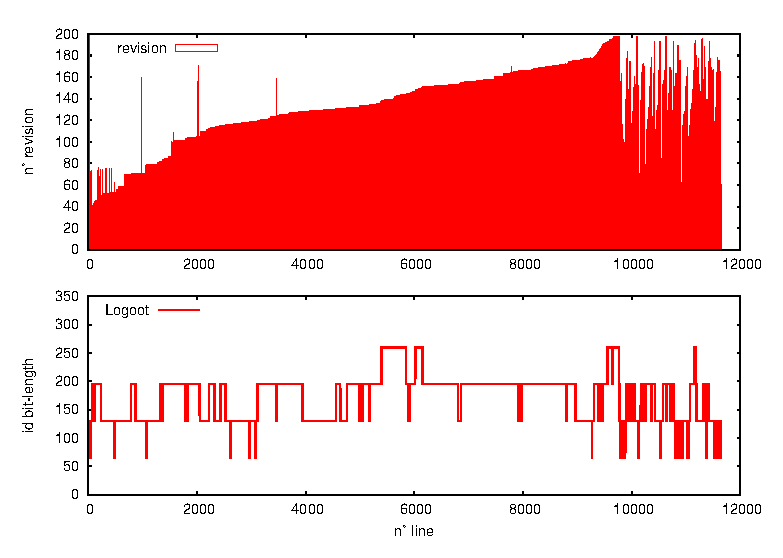
\includegraphics[width=0.48\textwidth]{./img/lseq/compliant.eps}}
  \hspace{10pt}
  \subfloat[Comportement d'édition inattendu]
  [\label{fig:lseq:motivating}Le comportement d'édition va à l'encontre des attentes
  de la stratégie d'allocation]
  {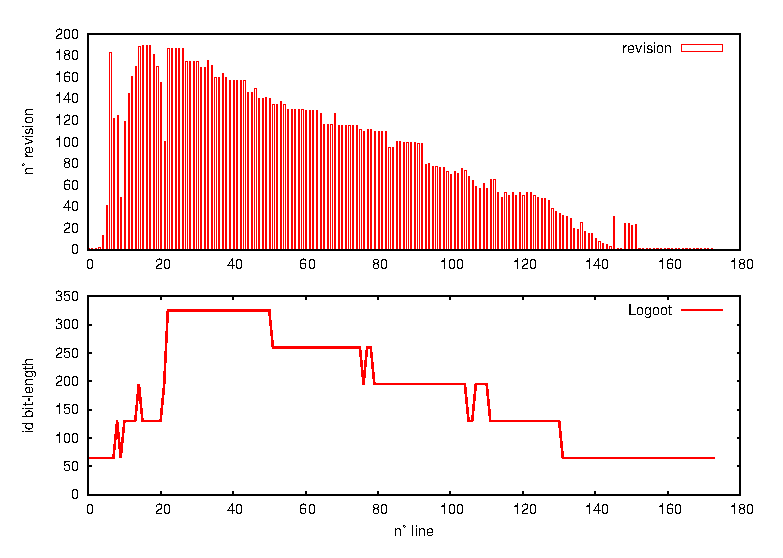
\includegraphics[width=0.48\textwidth]{./img/lseq/motivating.eps}}
  \caption{\label{fig:lseq:allocation}Spectre de documents Wikipedia sous différent
    comportements d'édition antagonistes. La figure du haut représente la
    révision à laquelle la ligne a été insérée, i.e., sa date de naissance.  La
    figure du bas représente la taille de l'identifiant associé à chaque ligne.}
\end{figure*}

Les figures~\ref{fig:lseq:compliant} et~\ref{fig:lseq:motivating} montrent deux
comportements d'éditions présent sur des pages extraites de Wikipedia. La partie
supérieure de ces figures donne une vue globale du comportement d'édition sur la
page. Elle indique la numéro de la révision à laquelle une ligne a été
insérée. Ainsi, plus une barre est haute, plus la ligne a été insérée
récemment. Le spectre de la figure~\ref{fig:lseq:compliant} montre que les
nouveaux éléments de la séquence sont principalement ajoutés en fin. À l'opposé,
le spectre de la figure~\ref{fig:lseq:motivating} montre que les nouveaux
éléments de la séquence sont principalement ajoutés en tête. La partie
inférieure de ces figures montre la taille de la représentation binaire de
l'identifiant associé à chaque élément du document. \TODO{Présenter la stratégie
  d'allocation}. Ainsi, nous observons que les identifiants dans le document
comportant 12k lignes mais principalement édité en fin a des identifiants
n'excédant pas 256 bits. En revanche, le document possédant seulement 170 lignes
édité en tête a des identifiants atteignant déjà les 320 bits.

\TODO{Définition du problème}

%%% Local Variables:
%%% mode: latex
%%% TeX-master: "../../paper"
%%% End:

%%
\section{LSEQ : une stratégie d'allocation polylogarithmique}

\LSEQ (abréviation pour \emph{polyLogarithimic SEQuence}) est une stratégie
d'allocation d'identifiants dont la taille est variable à la génération. Pour
générer ses identifiants immuables et uniques, \LSEQ utilise un arbre
exponentiel comme structure de données, deux sous-stratégies d'allocations avec
objectifs antagonistes, et un composant permettant de choisir la stratégie.

\subsection{Principe général}

Le principe général de \LSEQ consiste à amortir les mauvais choix d'identifiants
par un ensemble suffisant d'identifiants dont la taille est
satisfaisante. Puisqu'il n'existe pas de stratégie d'allocation parfaite sans
connaissance préalable de la séquence d'édition, \LSEQ cherche a être assez
général pour gérer la plupart des comportements d'édition.


\subsection{Arbre exponentiel}

Un arbre exponentiel est une structure d'arbre dont chaque élément de l'arbre
possède k-fois plus de fils que son parent. Par exemple, si l'on fixe $k$ à $2$,
un élément dont le parent possède $4$ fils en possède $8$. Dans ce cas, il y a
une augmentation quadratique du nombre de fils en fonction de la profondeur qui
s'ajoute à l'augmentation commune de l'arbre.

\TODO{figure}

Un identifiant \LSEQ est un suite d'entiers représentant le chemin de l'élément
dans l'arbre. Pour encoder cette suite d'entiers


\subsection{Sous-stratégies d'allocation}

\subsection{Choix de stratégie}

%%% Local Variables:
%%% mode: latex
%%% TeX-master: "../../paper"
%%% End:

%%
\section{Experimentations}

\subsection{Simulations}

%%% Local Variables:
%%% mode: latex
%%% TeX-master: "../../paper"
%%% End:

%%
\section{Conclusion}
\label{lseq:sec:conclusion}

%%% Local Variables:
%%% mode: latex
%%% TeX-master: "../../paper"
%%% End:


%%% Local Variables:
%%% mode: latex
%%% TeX-master: "../../paper"
%%% End:


\chapter{Un protocole d'échantillonnage aléatoire adaptatif}
\label{net:chap:spray}
\minitoc


% \lettrine{C}ommuniquer des informations d'une machine à une autre est un besoin
% ancien. Une solution se developpe rapidement sous l'impulsion du projet Arpanet
% qui deviendra plus tard la base de l'internet. Initialement créé dans le but de
% connecter une machine à une autre, l'échelle évolue afin d'impliquer plusieurs
% machines communicant entre elles. Il s'agit alors d'un réseau de communication.



% Les machines d'un réseau sont adressables : Grâce à une métadonnée, un message
% émis par une machine trouve un chemin jusqu'à la machine ciblée. Par exemple,
% une adresse IP (\emph{Internet Protocol}) permet de retrouver une machine de
% manière transparente : Les infrastructures sous-jacentes sur l'itinéraire entre
% les machines, tels que les routeurs, sont inconnues. Un réseau construit sur de
% telles adresses logiques est appelé réseau superposé (\emph{network
%   overlay}). Un réseau superposé peut être construit sur un autre réseau
% superposé.

\begin{figure}
  \begin{center}
    \begin{tikzpicture}[scale=1.2]
\newcommand\X{55pt}
\newcommand\Y{55pt}


\draw[fill=white] (0*\X,0*\Y) +(5pt, 5pt) rectangle +(-5pt, -5pt);
\draw[fill=white] (1*\X,0*\Y) +(5pt, 5pt) rectangle +(-5pt, -5pt);
\draw[<->] (5+0*\X, 0*\Y) -- (-5+1*\X, 0*\Y);
\draw (0.5*\X,-5-1*\Y) node[anchor=north, align=center]{2 peers; 2 arcs};

\begin{scope}[shift={(1.5*\X,0*\Y)}]
\draw[fill=white] (0*\X,0*\Y) +(5pt, 5pt) rectangle +(-5pt, -5pt);
\draw[fill=white] (1*\X,0*\Y) +(5pt, 5pt) rectangle +(-5pt, -5pt);
\draw[fill=white] (1*\X,-1*\Y) +(5pt, 5pt) rectangle +(-5pt, -5pt);
\draw[<->] (5+0*\X, 0*\Y) -- (-5+1*\X, 0*\Y);
\draw[<->] ( 1*\X, -5+0*\Y) -- ( 1*\X, 5-1*\Y);
\draw[<->] (5+0*\X, -5+0*\Y) -- (-5+1*\X, 5-1*\Y);
\draw (0.5*\X,-5-1*\Y) node[anchor=north, align=center]{3 peers; 6 arcs};
\end{scope}

\begin{scope}[shift={(3*\X,0*\Y)}]
\draw[fill=white] (0*\X,0*\Y) +(5pt, 5pt) rectangle +(-5pt, -5pt);
\draw[fill=white] (1*\X,0*\Y) +(5pt, 5pt) rectangle +(-5pt, -5pt);
\draw[fill=white] (1*\X,-1*\Y) +(5pt, 5pt) rectangle +(-5pt, -5pt);
\draw[fill=white] (0*\X,-1*\Y) +(5pt, 5pt) rectangle +(-5pt, -5pt);
\draw[<->] (5+0*\X, 0*\Y) -- (-5+1*\X, 0*\Y);
\draw[<->] ( 1*\X, -5+0*\Y) -- ( 1*\X, 5-1*\Y);
\draw[<->] (5+0*\X, -5+0*\Y) -- (-5+1*\X, 5-1*\Y);
\draw[<->] (5+0*\X, 5-1*\Y) -- (-5+1*\X, -5+0*\Y);
\draw[<->] (5+0*\X,-1*\Y) -- (-5+1*\X, -1*\Y);
\draw[<->] ( 0*\X,5-1*\Y) -- ( 0*\X, -5+0*\Y);
\draw (0.5*\X,-5-1*\Y) node[anchor=north, align=center]{4 peers; 12 arcs};
\end{scope}

\begin{scope}[shift={(4.5*\X,0*\Y)}]
\draw[fill=white] (0.33*\X,0*\Y) +(5pt, 5pt) rectangle +(-5pt, -5pt);
\draw[fill=white] (0.66*\X,0*\Y) +(5pt, 5pt) rectangle +(-5pt, -5pt);
\draw[fill=white] (0*\X,-0.5*\Y) +(5pt, 5pt) rectangle +(-5pt, -5pt);
\draw[fill=white] (1*\X,-0.5*\Y) +(5pt, 5pt) rectangle +(-5pt, -5pt);
\draw[fill=white] (0.5*\X,-1*\Y) +(5pt, 5pt) rectangle +(-5pt, -5pt);

\draw[<->] (-5+0.33*\X, 0*\Y) -- (0*\X,5-0.5*\Y);
\draw[<->] ( 5+0.66*\X, 0*\Y) -- (1*\X,5-0.5*\Y);
\draw[<->] (0.33*\X, -5+0*\Y) -- (0.5*\X, 5-1*\Y);
\draw[<->] (0.66*\X, -5+0*\Y) -- (0.5*\X, 5-1*\Y);
\draw[<->] (5+0*\X, 5-0.5*\Y) -- (-5+0.66*\X, -5-0*\Y);
\draw[<->] (-5+1*\X, 5-0.5*\Y) -- (5+0.33*\X, -5-0*\Y);
\draw[<->] (0*\X, -5-0.5*\Y) -- (-5+0.5*\X, -1*\Y);
\draw[<->] (1*\X, -5-0.5*\Y) -- (5+0.5*\X, -1*\Y);
\draw[<->] (5+0.33*\X, 0*\Y) -- (-5+0.66*\X, 0*\Y);
\draw[<->] (5+0*\X, -0.5*\Y) -- (-5+1*\X, -0.5*\Y);
\draw (0.5*\X,-5-1*\Y) node[anchor=north, align=center]{5 peers; 20 arcs};
\end{scope}


\end{tikzpicture}
    \caption[Graphes complets]{\label{net:fig:completegraph}Graphes complets.}
  \end{center}
\end{figure}

\lettrine{L}'édition collaborative~\cite{ellis1991groupware} permet de répartir
le travail de rédaction d'un document selon les trois dimensions : le temps,
l'espace, et les activités~\cite{desanctis1987foundation,
  grudin1994computersupported, johansen1988groupware}. L'éditeur collaboratif en
constitue l'outil principal récemment popularisé grâce aux éditeurs web tels que
\emph{Google Docs}~\cite{googledocs} ou \emph{ShareLatex}~\cite{sharelatex}. Ces
éditeurs proposent à leurs utilisateurs de créer et modifier un document en
temps réel. Grâce à un simple lien, ils sont en mesure de partager ce document à
des amis ou des collègues. Ces derniers sont à leur tour capables de lire et
modifier le document en temps réel.

Les utilisateurs impliquées dans l'édition peuvent être éloignés les uns des
autres géographiquement. Par exemple, un japonais, un français et un brésilien
peuvent éditer un même document en temps réel depuis leur pays d'origine. Cette
répartition géographique necessite l'établissement de moyens de communication
entre éditeurs.
%% De plus, web -> masse
Chaque modification doit parvenir efficacement au reste des participants afin
que le même document puisse être lu partout.

Un réseau superposé (\emph{network overlay}) est un ensemble de machines pouvant
communiquer entre elles au dessus d'un autre réseau tels que, par exemple,
l'internet ou un autre réseau superposé.  Toutes sortes de réseaux superposés
existent. Si chaque machine possède un canal de communication avec chacune des
autres machines, alors la topologie correspond à celle d'un graphe complet
(cf. figure~\ref{net:fig:completegraph}). La progression quadratique du nombre
d'arcs en fonction du nombre de nœuds empêche un tel système d'atteindre de
grandes envergures. Afin de résoudre ce problème, les machines ne possèdent
qu'une vue partielle du réseau. Cette vue partielle constitue le voisinage
direct d'un nœud. Le défi consiste alors à peupler ces vues avec des liens
logiques selon les critères souhaités.

Dans ce manuscrit, nous nous intéressons aux protocoles d'échantillonnage
aléatoire de pairs~\cite{jelasity2007gossip} dont l'objectif est de fournir à
chaque machine une vue partielle peuplée d'adresses logiques réparties selon une
loi uniforme. La topologie en résultant est proche de celle des graphes
aléatoires~\cite{erdos1959random}. Ces réseaux possèdent d'intéressantes
propriétés tels que la tolérance aux pannes ou un faible diamètre. Cette
première garantie que lorsqu'un nœud disparaît soudainement le graphe reste
connecté avec une forte probabilité, la seconde garantie que les messages se
propagent rapidement à tous les membres du réseau.

% Puisque les protocoles de dissémination de messages font un usage soutenu de ces
% vues partielles, améliorer le protocole d'échantillonnage revient à améliorer la
% dissémination. Le problème scientifique consiste à 

L'état de l'art des protocoles d'échantillonnage aléatoire de pairs se divise en
deux catégories selon les vues partielles fournies :
\begin{inparaenum}[(i)]
\item les approches fournissant des vues partielles de taille
  constante~\cite{eugster2003lightweight, leitao2007dependable,
    tolgyeski2009adaptive, voulgaris2005cyclon} qui doivent être configurées
  \emph{a priori}. Dans ce cas le développeur doit prévoir les dimensions des
  réseaux gérés par son application;
  %%Cela entraîne un  surdimensionnement des vues partielles.
\item les approches fournissant des vues partielles s'auto-ajustant pendant la
  vie du réseau~\cite{ganesh2001scamp, ganesh2003peer}. Malheureusement, ces
  approches ne sont pas adaptées aux réseaux dynamiques.
\end{inparaenum}

Les protocoles d'échantillonnages aléatoire de pairs sont au cœur de nombreuses
autres approches~\cite{folz2016cyclades, jelasity2009tman,
  krasikova2016distributed, voulgaris2013vicinity}. Entre autres, la propagation
de messages~\cite{birman1999bimodal, kermarrec2003probabilistic} d'un pair à
tous les autres (\emph{broadcast}) fait un usage intensif des vues
partielles. Un pair souhaitant propager un message choisit un ensemble de
voisins auquel il communique le message. A son tour, chaque pair recevant un tel
message en fait de même. Les messages parviennent à tous les pairs par
transitivité à la manière d'une épidémie.

Afin d'adapter le trafic généré par la transmission de messages, \textbf{comment
  adapter efficacement le voisinage de chaque éditeur au nombre fluctuant de
  collaborateurs ?}

Ce chapitre présente \SPRAY~\cite{nedelec2015spray}, un protocole dont les pairs
voient leur vue partielle s'ajuster gracieusement à la taille du réseau, sans
l'usage d'aucune connaissance globale. Le cycle de vie d'un pair, divisé entre
son entrée, sa vie, et son départ, est conçu pour conserver un nombre d'arcs
dans le système consistant avec la taille de ce dernier. Les protocoles
construits au dessus de \SPRAY peuvent bénéficier de cette auto-ajustement. Par
exemple, le trafic généré par un protocole de dissémination de messages peut
évoluer selon les dimensions du réseau.

Ce chapitre commence par introduire vocabulaire et notations. La
section~\ref{net:sec:stateoftheart} présente l'état de l'art des protocoles
d'échantillonnage de pairs en les divisant en deux catégories : ceux dont les
vues partielles sont fixes, et ceux dont les vues partielles s'adaptent au
réseau. La section~\ref{net:sec:spray} présente \SPRAY, un protocole appartenant
à la seconde catégorie. La section~\ref{net:sec:properties} présente et compare
les propriétés des protocoles d'échantillonnages. La
section~\ref{net:sec:usecase} présente l'effet de \SPRAY sur un protocole de
dissémination épidémique de messages. Le chapitre se conclut à la
section~\ref{net:sec:conclusion}.

%%% Local Variables:
%%% mode: latex
%%% TeX-master: "../../paper"
%%% End:




\section{État de l'art}
\label{net:sec:stateoftheart}


Un réseau superposé permet à un ensemble de machines de communiquer entre elles
au dessus d'un autre réseau tels que, par exemple, l'internet ou un autre réseau
superposé.  Toutes sortes de réseaux superposés existent. Si chaque machine
possède un canal de communication avec chacune des autres machines, alors la
topologie correspond à celle d'un graphe complet
(cf. figure~\ref{net:fig:completegraph}). La progression quadratique du nombre
d'arcs en fonction du nombre de nœuds empêche un tel système d'atteindre de
grandes envergures. Afin de résoudre ce problème, les machines ne possèdent
qu'une vue partielle du réseau. Cette vue partielle constitue le voisinage
direct d'un nœud. Le défi consiste alors à peupler ces vues avec des liens
logiques selon les critères souhaités.


Dans ce manuscrit, nous nous intéressons aux protocoles d'échantillonnage
aléatoire de pairs~\cite{jelasity2007gossip} dont l'objectif est de fournir à
chaque machine une vue partielle peuplée d'adresses logiques réparties selon une
loi uniforme. La topologie en résultant est proche de celle des graphes
aléatoires~\cite{erdos1959random}. Ces réseaux possèdent d'intéressantes
propriétés tels que la tolérance aux pannes ou un faible diamètre. Cette
première garantit que lorsqu'un nœud disparaît soudainement le graphe reste
connecté avec une forte probabilité, la seconde garantie que les messages se
propagent rapidement à tous les membres du réseau.


Deux familles d'approches existent quant à la taille des vues partielles :
\begin{inparaenum}[(i)]
\item La famille d'approches dont la taille est fixée lors de la
  configuration. Ainsi la taille des vues partielles ne change pas au cours du
  temps, même si la taille du réseau est susceptible de fluctuer
  (cf. §\ref{net:subsec:fixed}).
\item La famille dont les machines, lorsqu'elles rejoignent le réseau,
  contribuent à hauteur du logarithme de la taille du réseau
  (cf. §\ref{net:subsec:variable}).
\end{inparaenum}

\subsection{Taille fixe}
\label{net:subsec:fixed}

Les protocoles d'échantillonnage aléatoire de pairs peuplant des vues dont la
taille est constante possèdent un socle commun à savoir l'échanges périodiques
de voisinages.

\paragraph{\CYCLON~\cite{voulgaris2005cyclon} :} est un protocole où chaque nœud
possède une vue partielle dont chaque arc est associé à un âge. Régulièrement,
les nœuds initient un mélange (\emph{shuffling}) avec leur voisin le plus
âgé. Si la communication est possible, le processus est amorcé et l'âge de tous
les voisins est incrémenté, sinon l'adresse est supprimée. Cela permet de
supprimer les nœuds considérés comme partis.

\noindent Lors de ce mélange, le nœud envoie un nombre prédéfinit de ses arcs au
nœud choisit, en prenant soin de remplacer l'arc vers son homologue par la
sienne propre. Les adresses sont choisies aléatoirement. À la réception, son
vis-à-vis choisit un nombre d'arcs équivalent et les lui envoie. Les deux nœuds
intègrent alors l'ensemble qu'ils ont reçu. Lorsque l'ensemble obtenu est trop
grand pour la taille de vue partielle prédéfinie, des arcs sont rejetés en
conservant de préférence les nouveaux arcs reçus et en supprimant les doublons.
  
\begin{figure}
  \centering
  \subfloat[Choix aléatoire des pairs dans \CYCLON]
  [\label{net:fig:cyclonexampleA} L'initiateur du mélange choisit d'envoyer $n_5$ et lui-même à son plus vieux voisin $n_2$. En retour, il lui propose $n_6$ et $n_7$.]
  {\begin{tikzpicture}[scale=1.2]
\newcommand\X{45pt}
\newcommand\Y{20pt}


\draw[fill=white, draw=darkblue]( 0*\X, -2*\Y)
node{\DARKBLUE{$n_1$}} +(5pt, 5pt) rectangle +(-5pt,-5pt);
\draw[fill=white]( 1*\X, -2*\Y) node{$n_2$} +(5pt, 5pt) rectangle +(-5pt,-5pt);


\draw[fill=white](-1*\X, 0*\Y) node{$n_3$} +(5pt, 5pt) rectangle +(-5pt,-5pt);
\draw[fill=white](-1*\X, -1*\Y) node{$n_4$} +(5pt, 5pt) rectangle +(-5pt,-5pt);
\draw[fill=white, draw=darkblue](-1*\X, -3*\Y)
node{\DARKBLUE{$n_5$}} +(5pt, 5pt) rectangle +(-5pt,-5pt);

\draw[fill=white, draw=darkblue]( 2*\X, -0*\Y)
node{\DARKBLUE{$n_6$}} +(5pt, 5pt) rectangle +(-5pt,-5pt);
\draw[fill=white, draw=darkblue]( 2*\X, -1*\Y)
 node{\DARKBLUE{$n_7$}} +(5pt, 5pt) rectangle +(-5pt,-5pt);
\draw[fill=white]( 2*\X, -3*\Y) node{$n_8$} +(5pt, 5pt) rectangle +(-5pt,-5pt);
\draw[fill=white]( 2*\X, -4*\Y) node{$n_9$} +(5pt, 5pt) rectangle +(-5pt,-5pt);

\draw[->] (-5+0*\X, -2*\Y) -- (5-1*\X, 0*\Y);
\draw[->] (-5+0*\X, -2*\Y) -- (5-1*\X, -1*\Y);
\draw[->] (-5+0*\X, -2*\Y) -- (5-1*\X, -3*\Y);

\small
\draw[->] (5+0*\X, -2*\Y) -- node[anchor=south]{ancien} (-5+1*\X, -2*\Y);

\draw[->] (5+1*\X, -2*\Y) -- (-5+2*\X, 0*\Y);
\draw[->] (5+1*\X, -2*\Y) -- (-5+2*\X, -1*\Y);
\draw[->] (5+1*\X, -2*\Y) -- (-5+2*\X, -3*\Y);
\draw[->] (5+1*\X, -2*\Y) -- (-5+2*\X, -4*\Y);
\end{tikzpicture}}
  \hspace{35pt}
  \subfloat[Établissement des connexions après le mélange dans \CYCLON]
  [\label{net:fig:cyclonexampleB} Les arcs sont échangés de part et d'autre.]
  {\begin{tikzpicture}[scale=1.2]
\newcommand\X{45pt}
\newcommand\Y{20pt}


\draw[fill=white]( 0*\X, -2*\Y) node{$n_1$} +(5pt, 5pt) rectangle +(-5pt,-5pt);
\draw[fill=white]( 1*\X, -2*\Y) node{$n_2$} +(5pt, 5pt) rectangle +(-5pt,-5pt);


\draw[fill=white](-1*\X, 0*\Y) node{$n_3$} +(5pt, 5pt) rectangle +(-5pt,-5pt);
\draw[fill=white](-1*\X, -1*\Y) node{$n_4$} +(5pt, 5pt) rectangle +(-5pt,-5pt);
\draw[fill=white](-1*\X, -3*\Y) node{$n_5$} +(5pt, 5pt) rectangle +(-5pt,-5pt);

\draw[fill=white]( 2*\X, -0*\Y) node{$n_6$} +(5pt, 5pt) rectangle +(-5pt,-5pt);
\draw[fill=white]( 2*\X, -1*\Y) node{$n_7$} +(5pt, 5pt) rectangle +(-5pt,-5pt);
\draw[fill=white]( 2*\X, -3*\Y) node{$n_8$} +(5pt, 5pt) rectangle +(-5pt,-5pt);
\draw[fill=white]( 2*\X, -4*\Y) node{$n_9$} +(5pt, 5pt) rectangle +(-5pt,-5pt);

\draw[->] (-5+0*\X, -2*\Y) -- (5-1*\X, 0*\Y);
\draw[->] (-5+0*\X, -2*\Y) -- (5-1*\X, -1*\Y);
% \draw[->] (-5+0*\X, -2*\Y) -- (5-1*\X, -3*\Y);
\draw[->, color=darkblue] (5+0*\X, 5-2*\Y) -- (-5+2*\X, 0*\Y);
\draw[->, color=darkblue] (5+0*\X, 5-2*\Y) -- (-5+2*\X, -1*\Y);


\draw[<-, darkblue] (5+0*\X, -2*\Y) -- (-5+1*\X, -2*\Y);

\draw[->, color=darkblue] (-5+1*\X, -5-2*\Y) -- (5-1*\X, -3*\Y);
% \draw[->] (5+1*\X, -2*\Y) -- (-5+2*\X, 0*\Y);
% \draw[->] (5+1*\X, -2*\Y) -- (-5+2*\X, -1*\Y);
\draw[->] (5+1*\X, -2*\Y) -- (-5+2*\X, -3*\Y);
\draw[->] (5+1*\X, -2*\Y) -- (-5+2*\X, -4*\Y);
\end{tikzpicture}}
  \caption[Exemple de mélange dans \CYCLON]
  {\label{net:fig:cyclonexample} Exemple de mélange par \CYCLON. Pour
    améliorer la lisibilité, seuls les vues partielles du $n_1$ et $n_2$ sont
    explicitées.}
\end{figure}
  
\noindent La figure~\ref{net:fig:cyclonexample} décrit un exemple de mélange
initié par le nœud $n_1$. Dans cet exemple, les vues partielles sont configurées
pour accueillir 4 arcs et en échanger 2 pendant les mélanges. La
figure~\ref{net:fig:cyclonexampleA} montre que $n_1$ choisit son plus vieux
voisin afin d'initier l'échange, à savoir $n_2$. Il incorpore dans l'échange sa
propre identité ainsi que celle d'un arc connu aléatoirement. Le nœud $n_2$
reçoit la demande de mélange et choisit 2 nœuds aléatoirement, ici $n_6$ et
$n_7$ qu'il envoie à son tour. La figure~\ref{net:fig:cyclonexampleB} montre que
les nœuds participants au mélange ont supprimé les arcs qu'ils ont envoyé et
ajouté ceux nouvellement reçu. En particulier, l'inversion de l'arc ayant permis
le mélange garantit que le graphe reste connexe.

\paragraph{Newscast~\cite{tolgyeski2009adaptive} :} est un protocole où les vues
partielles associent à chaque arc une estampille
(\emph{timestamp}). Périodiquement, les nœuds de Newscast effectuent un mélange
périodique. Pour cela, ils choisissent l'un de leurs voisins aléatoirement et
envoient la totalité de leur vue partielle à laquelle est ajoutée leur propre
identité associée à une estampille à jour. Lors de la réception, leur homologue
en fait de même. Tout deux fusionnent leur table de voisinage de telle sorte que
seules les entrées les plus récentes selon l'estampille sont conservées.

\noindent Un nœud qui quitte le réseau n'effectue plus ce mélange périodique et
ainsi n'annonce plus sa présence au reste du réseau. Petit à petit, les vues
partielles possédant un arc pointant vers ce nœud s'en débarrassent car l'arc
est devenu obsolète en comparaison des arcs nouvellement reçus.

\noindent Les pertes de messages dues à la non-fiabilité des communications
mettent en dangers la distribution des arcs. Par exemple, si un message sur deux
est perdu lorsqu'un certain nœuds tente de communiquer, il perd tout autant
d'occasions de s'annoncer au réseau. Par conséquent, il encourt le risque d'être
évincé de certaines vues partielles, voir de disparaître complètement. En
d'autres termes, le nœud est moins bien connecté que les autres à cause de ces
messages perdus. Newscast propose de compenser cela. Ainsi, si un nœud perd un
message sur deux, il émet deux fois plus. La distribution des arcs s'en trouve
ajustée.

\begin{figure}
  \centering
  \subfloat[Initiation du mélange dans Newscast]
  [\label{net:fig:newscastexampleA} L'initiateur du mélange $n_2$ aléatoirement et lui envoie sa vue à laquelle il s'ajoute avec une estampille à jour. À la réception, $n_2$ en fait de même.]
  {\begin{tikzpicture}[scale=1.2]
\newcommand\X{45pt}
\newcommand\Y{20pt}


\draw[fill=white, draw=darkblue]( 0*\X, -2*\Y)
node{\DARKBLUE{$n_1$}} +(5pt, 5pt) rectangle +(-5pt,-5pt);
\draw[fill=white, draw=darkblue]( 1*\X, -2*\Y)
node{\DARKBLUE{$n_2$}} +(5pt, 5pt) rectangle +(-5pt,-5pt);


\draw[fill=white, draw=darkblue](-1*\X, 0*\Y)
node{\DARKBLUE{$n_3$}} +(5pt, 5pt) rectangle +(-5pt,-5pt);
\draw[fill=white, draw=darkblue](-1*\X, -1*\Y)
node{\DARKBLUE{$n_4$}} +(5pt, 5pt) rectangle +(-5pt,-5pt);
\draw[fill=white, draw=darkblue](-1*\X, -3*\Y)
node{\DARKBLUE{$n_5$}} +(5pt, 5pt) rectangle +(-5pt,-5pt);

\draw[fill=white, draw=darkblue]( 2*\X, -0*\Y)
node{\DARKBLUE{$n_6$}} +(5pt, 5pt) rectangle +(-5pt,-5pt);
\draw[fill=white, draw=darkblue]( 2*\X, -1*\Y)
 node{\DARKBLUE{$n_7$}} +(5pt, 5pt) rectangle +(-5pt,-5pt);
\draw[fill=white, draw=darkblue]( 2*\X, -3*\Y)
node{\DARKBLUE{$n_8$}} +(5pt, 5pt) rectangle +(-5pt,-5pt);
\draw[fill=white, draw=darkblue]( 2*\X, -4*\Y)
node{\DARKBLUE{$n_9$}} +(5pt, 5pt) rectangle +(-5pt,-5pt);

\scriptsize

\draw[->] (-5+0*\X, -2*\Y) -- node[anchor=west]{13:12} (5-1*\X, 0*\Y);
\draw[->] (-5+0*\X, -2*\Y) -- node[anchor=north east]{13:15} (5-1*\X, -1*\Y);
\draw[->] (-5+0*\X, -2*\Y) -- node[anchor=north west]{13:16} (5-1*\X, -3*\Y);

\small

\draw[->] (5+0*\X, -2*\Y) -- node[anchor=south]{aléatoire} (-5+1*\X, -2*\Y);

\scriptsize

\draw[->] (5+1*\X, -2*\Y) -- node[anchor=south east]{13:13} (-5+2*\X, 0*\Y);
\draw[->] (5+1*\X, -2*\Y) -- node[anchor=north west]{13:13} (-5+2*\X, -1*\Y);
\draw[->] (5+1*\X, -2*\Y) -- node[anchor=south west]{13:14} (-5+2*\X, -3*\Y);
\draw[->] (5+1*\X, -2*\Y) -- node[anchor=north east]{13:17} (-5+2*\X, -4*\Y);
\end{tikzpicture}}
  \hspace{35pt}
  \subfloat[Établissement des connexions après le mélange dans Newscast]
  [\label{net:fig:newscastexampleB} Les arcs sont échangés de part et d'autre en conservant les estampilles les plus récentes.]
  {\begin{tikzpicture}[scale=1.2]
\newcommand\X{45pt}
\newcommand\Y{20pt}


\draw[fill=white]( 0*\X, -2*\Y) node{$n_1$} +(5pt, 5pt) rectangle +(-5pt,-5pt);
\draw[fill=white]( 1*\X, -2*\Y) node{$n_2$} +(5pt, 5pt) rectangle +(-5pt,-5pt);


\draw[fill=white](-1*\X, 0*\Y) node{$n_3$} +(5pt, 5pt) rectangle +(-5pt,-5pt);
\draw[fill=white](-1*\X, -1*\Y) node{$n_4$} +(5pt, 5pt) rectangle +(-5pt,-5pt);
\draw[fill=white](-1*\X, -3*\Y) node{$n_5$} +(5pt, 5pt) rectangle +(-5pt,-5pt);

\draw[fill=white]( 2*\X, -0*\Y) node{$n_6$} +(5pt, 5pt) rectangle +(-5pt,-5pt);
\draw[fill=white]( 2*\X, -1*\Y) node{$n_7$} +(5pt, 5pt) rectangle +(-5pt,-5pt);
\draw[fill=white]( 2*\X, -3*\Y) node{$n_8$} +(5pt, 5pt) rectangle +(-5pt,-5pt);
\draw[fill=white]( 2*\X, -4*\Y) node{$n_9$} +(5pt, 5pt) rectangle +(-5pt,-5pt);

\scriptsize

% \draw[->] (-5+0*\X, -2*\Y) -- (5-1*\X, 0*\Y);
\draw[->] (-5+0*\X, -2*\Y) -- (5-1*\X, -1*\Y)
node[anchor=west]{\ 13:15};
\draw[->] (-5+0*\X, -2*\Y) -- (5-1*\X, -3*\Y);



\draw[->, color=darkblue] (5+0*\X, -5 -2*\Y) -- (-5+2*\X, -4*\Y)
node[anchor=east]{13:17\ };

\draw[<->, color=darkblue] (5+0*\X, -2*\Y) --
node[anchor=south]{13:18}(-5+1*\X, -2*\Y);

\draw[->, color=darkblue] (-5+1*\X, -5-2*\Y) -- (5-1*\X, -3*\Y)
node[anchor=west]{\ 13:16};
% \draw[->] (5+1*\X, -2*\Y) -- (-5+2*\X, 0*\Y);
% \draw[->] (5+1*\X, -2*\Y) -- (-5+2*\X, -1*\Y);
% \draw[->] (5+1*\X, -2*\Y) -- (-5+2*\X, -3*\Y);
\draw[->] (5+1*\X, -2*\Y) -- (-5+2*\X, -4*\Y);
\end{tikzpicture}}
  \caption[Exemple de mélange dans Newscast]
  {\label{net:fig:newscastexample} Exemple de mélange par Newscast. Ici, les
    estampilles sont simplement formatées hh:mm.}
\end{figure}

\noindent La figure~\ref{net:fig:newscastexample} montre un exemple de mélange
avec le protocole Newscast. Là encore, la taille des vues partielles est fixée à
4 entrées. Le nœud $n_1$ initie le mélange avec un voisin choisit aléatoirement
: $n_2$. Il envoie l'intégralité de sa vue à laquelle il s'ajoute avec
l'estampille actuelle 13:18. Le nœud $n_2$ le reçoit et en fait de même. Les
deux nœuds $n_1$ et $n_2$ conservent les quatre arcs les plus récents qu'ils
possèdent, à savoir les arcs vers leur homologue, $n_4$, $n_5$ et $n_9$. La
figure~\ref{net:fig:newscastexampleB} nous permet de remarquer que le réseau
semble collapser. En particulier, certains nœuds ne sont plus référencés ni par
$n_1$, ni par $n_2$. Toutefois, il ne s'agit là que de la représentation locale
au mélange. Globalement, la topologie résultante reste proche de celle des
graphes aléatoires.

\paragraph{Lpbcast~\cite{eugster2003lightweight} :} est le diminutif de
\emph{lightweight probabilistic broadcast}. C'est un protocole dont les vues
partielles ne comprennent que des arcs sans metadonnées additionnelles. C'est
lorsqu'un nœud diffuse un message au réseau que les vues sont mises à
jour. Chaque message comporte un ensemble borné d'identités de nœuds ayant
quitté le réseau, et un ensemble borné d'identités de nœuds échantillonnés au
cours du cheminement du message. Si aucun message n'a été reçu ni envoyé dans un
certain intervalle de temps, une diffusion est automatiquement générée afin
d'activer le mécanisme de mélange.

\noindent Lors de la réception de tels messages, un nœud peuple sa propre vue
partielle des nouveaux éléments présent dans le message avant de la réajuster à
la taille maximale autorisée en supprimant aléatoirement des arcs.

\paragraph{HyParView~\cite{leitao2007dependable} :} est un protocole possédant
deux vues partielles. La première est active et est utilisée lors de l'émission
de messages au réseau. La seconde est passive et sert à remplacer les arcs
obsolètes de la vue active, e.g., lors d'une défaillance ou d'un départ
volontaire.  La vue active est considérablement plus petite que la vue passive
et les arcs compris dans cette première sont vérifiés à chaque message émit.

\noindent Lors d'un mélange, les arcs contenus dans les deux vues sont sujets à
échange dans le but de supprimer les nœuds défaillants de toutes les vues
passives. Similairement à \CYCLON, les arcs privilégiés sont ceux nouvellement
reçus.


Les approches appartenant à la famille dont les vues partielles
sont constantes ne sont pas adaptées aux contextes avec :

\paragraph{Un même réseau.} La taille d'un réseau fluctue au cours du temps. Par
exemple, lorsque les utilisateurs possèdent des habitudes identiques, il peut
alors y avoir des heures creuses où le réseau ne compte que peu de membres. À
l'inverse, lors d'événements particuliers, beaucoup d'entrées en très peu de
temps peuvent avoir lieu. Le web amplifie ces fluctuations. En effet, le web
favorise la diffusion d'idées. Par exemple, dans le cadre de l'édition
collaborative, un simple lien HTTP permet le partage d'un document. Un lien
\emph{tweeté} par une célébrité sur un événement particulier peut attirer des
milliers de participants en très peu de temps. Cette soudaine popularité retombe
lorsque l'événement s'achève.  Pour gérer ces cas, les approches fournissant des
vues dont la taille est configurée \emph{a priori} doivent être pessimistes :
les vues partielles sont surdimensionnées afin de supporter ces cas
éphémères. Les protocoles qui dépendent, tel que la dissémination de messages,
héritent de ce pessimisme qui les conduit à, par exemple, produire un trafic
excessif lorsque le réseau est plus modeste que prévu.


\paragraph{Plusieurs réseaux.} La taille des réseaux créés par une même
application varie. Par exemple, un document partagé pour un événement de grande
ampleur n'a pas la même audience qu'un document partagé avec quelques
amis. Malgré tout, le développeur d'application doit prévoir large afin de
supporter les grands groupes s'ils existent, au détriment des plus petits
groupes d'utilisateurs.


%\TODO{Maybe talk about estimators\ldots}

% TRANSITION


\subsection{Taille variable}
\label{net:subsec:variable}

La famille de protocoles d'échantillonnage aléatoire de pairs peuplant des vues
dont la taille n'est pas définie au préalable a pour seul représentant :

\paragraph{\SCAMP~\cite{ganesh2001scamp, ganesh2003peer} :} est l'acronyme de
\emph{SCAlable Membership Protocol}. Il s'agit d'un protocole d'échantillonnage
associant une réaction à certains événements. En particulier, l'entrée dans le
réseau doit permettre d'augmenter la taille moyenne des vues partielles. Cette
augmentation est logarithmique. Le départ d'un nœud doit entraîner une
équivalente diminution.

\noindent Les pairs utilisant \SCAMP maintiennent deux vues partielles
correspondants aux arcs entrant et aux arcs sortant.

\noindent Lorsque un nœud rejoint le réseau, il contacte un membre qu'il ajoute
directement à sa vue partielle. Ce contact annonce ensuite le nouveau venu au
réseau. Pour ce faire, il crée autant de messages d'annonce qu'il possède de
voisins et les dissémine. Chaque nœud recevant ce type de messages est libre
d'accepter l'annonce en ajoutant alors l'identité du nouveau venu à sa vue
partielle, ou la refuser, auquel cas il réexpédie le message à l'un de ces
voisins. Afin de répartir équitablement les annonces, chaque nœud $n_i$ a une
probabilité inversement proportionnelle à la taille de sa vue partielle
d'accepter l'annonce : $1/(|P_i|+1)$. Cette répartition des arcs seules permet
de créer une topologie proche de celle des graphes aléatoires. Cependant, la vue
partielle du nouveau nœud est faiblement peuplée au contraire des nœuds plus
vieux. Cela met en danger la robustesse du réseau face aux défaillances.

\begin{figure}
  \centering
  
\begin{tikzpicture}[scale=1.3]
  
  \draw[fill=white, draw=darkblue] (0pt, 0pt)
  node{\DARKBLUE{$n_1$}} +(-5pt,-5pt) rectangle +(5pt,5pt);

  \begin{scope}[shift={(75pt,0pt)}]
  \draw[fill=white] (-25pt, 0pt) node{$n_2$} +(-5pt,-5pt) rectangle +(5pt,5pt);
  \draw[fill=white] (0pt,  25pt) node{$n_3$} +(-5pt,-5pt) rectangle +(5pt,5pt);
  \draw[fill=white] ( 25pt, 0pt) node{$n_4$} +(-5pt,-5pt) rectangle +(5pt,5pt);
  \draw[fill=white] (0pt, -25pt) node{$n_5$} +(-5pt,-5pt) rectangle +(5pt,5pt);


  \draw[->] (-20pt, 5pt) -- (-5pt, 20pt); 
  \draw[->] (-20pt,-5pt) -- (-5pt,-20pt); 
  \draw[->] ( 5pt,-20pt) -- (20pt, -5pt); 
  \draw[->] (20pt,  0pt) -- (-20pt, 0pt); 
  \draw[->] (-5pt, 30pt) -- (-30pt, 5pt); 

  \draw[->, color=darkblue] (-70pt, 0pt) -- (-30pt, 0pt); 
  \draw[->, color=darkblue] (-5pt, 30pt) -- (-70pt, 5pt); 
  \draw[->, color=darkblue] (30pt, -5pt)to[out=-85,in=-95](-70pt,-5pt);

  \scriptsize
  \draw (-25pt,-5pt) node[align=left,anchor=north east]
  {dissémine\\$|P_2|$ copies};
  \draw (5pt,-30pt) node[align=left,anchor=north west]
  {$1/2$ chance d'accepter,\\refuse, fait suivre à $n_4$};
  \draw (5pt, 30pt) node[align=left,anchor=south west]
  {$1/2$ chance d'accepter,\\accepte, crée $n_3 \rightarrow n_1$};
  \draw (30pt, 0pt) node[align=left,anchor=west]
  {$1/2$ chance d'accepter,\\accepte, crée $n_4 \rightarrow n_1$};
  \end{scope}
  
%%  \small
%%  \begin{scope}[shift={(130pt,0pt)}]
%%    \draw[fill=white](5pt, 0pt)node{$p_x$}+(-5pt,-5pt) rectangle +(5pt,5pt);
%%    \draw (10pt,0pt) node[anchor=west]{Peer $p_x$};
%%    \draw[->](0pt, -12pt)--(10pt, -12pt) node[anchor=west]{Established link};
%%    \draw[->, densely dashed](0pt, -19pt)--(10pt, -19pt)
%%    node[anchor=west]{New link};
%%    
%%  \end{scope}
  
\end{tikzpicture}
  \caption[Entrée dans un réseau dans \SCAMP]
  {\label{net:fig:scampexample} Exemple de nœud rejoignant le réseau dans
    \SCAMP.}
\end{figure}

\noindent La figure~\ref{net:fig:scampexample} montre l'entrée d'un nœud $n_1$
dans un petit réseau \SCAMP composé des nœuds $n_2$, $n_3$, $n_4$ et $n_5$. Dans
cet exemple, le nœud $n_1$ contacte $n_2$ et l'ajoute directement à sa vue
partielle. $n_2$, possédant 2 voisins, copie l'identité de $n_1$ 2 fois et les
dissémine à $n_3$ et $n_5$. Lorsque $n_3$ reçoit le message, il possède une
chance sur deux d'accepter l'annonce, ce qu'il fait : un arc est ajouté entre
$n_3$ et $n_1$. Le nœud $n_5$ procède de la même façon. Toutefois, il n'accepte
pas l'annonce et retransmet le message à son voisin $n_4$. Ce dernier l'accepte
et l'arc allant de $n_4$ à $n_1$ est créé. Au total, 3 arcs ont été créés à
l'arrivée du nœud $n_1$.


\noindent Lorsqu'un nœud souhaite quitter le réseau,
\begin{inparaenum}[(i)]
\item il œuvre à préserver la connectivité de ce dernier et
\item il emporte avec lui une quantité d'arcs correspondant à l'entrée du
  dernier nœud dans le réseau.
\end{inparaenum}
Pour ce faire, le nœud va agir comme pont entre les nœuds de sa vue partielle
entrante et ceux de sa vue partielle sortante. Ainsi, il permettra de ressouder
la maille du réseau qu'il aurait défait en partant. Ce mécanisme est
généralement applicable à tous les protocoles d'échantillonnage mais il requière
de maintenir deux vues partielles -- entrante et sortante -- et des canaux de
communication bidirectionnels. Il requière aussi un travail supplémentaire de la
part du nœud sortant impossible à garantir lors de défaillances : le nœud devra
servir d'intermédiaire à la connexion de tous les voisins de sa vue partielle
entrante (sauf un) vers autant de voisins appartenant à sa vue partielle
sortante. Ainsi, le nombre d'arcs supprimé correspond en moyenne à celui injecté
à l'entrée d'un nœud dans le réseau. Ce mécanisme améliore considérablement le
maintient de la connexité du réseau mais ne représente pas une solution fiable
pour autant. En effet, certains nœuds peuvent se trouver sans voisins dans l'une
de leurs vues partielles.
  

\begin{figure}
  \centering
  \subfloat[Départ d'un nœud avec \SCAMP.]
  [\label{net:fig:scampexampleB} Le nœud $n_1$ souhaite quitter le réseau. Il
  en informe ses vues partielles afin d'effectuer un pont entre eux.]
  {
\begin{tikzpicture}[scale=1.2]

  \newcommand\X{55pt};
  \newcommand\Y{15pt};

  \draw[<-](5+0*\X, -2*\Y)--(-5+1*\X, 0*\Y);
  \draw[<-](5+0*\X, -2*\Y)--(-5+1*\X, -1*\Y);
  \draw[<-](5+0*\X, -2*\Y)--(-5+1*\X, -3*\Y);

  \draw[->](-5+0*\X, -2*\Y)--(5-1*\X, 0*\Y);
  \draw[->](-5+0*\X, -2*\Y)--(5-1*\X, -1*\Y);
  \draw[->](-5+0*\X, -2*\Y)--(5-1*\X, -3*\Y);
  \draw[->](-5+0*\X, -2*\Y)--(5-1*\X, -4*\Y);

  \small
  \draw[fill=white,very thick, draw=darkblue]
  (0*\X, -2*\Y) node{\DARKBLUE{$n_1$}} +(-5pt,-5pt) rectangle +(5pt,5pt);
  \draw[thick, color=darkblue] (-5pt,-5-2*\Y) -- (5pt,5-2*\Y);
  \draw[thick, color=darkblue] (-5pt, 5-2*\Y) -- (5pt,-5-2*\Y);
  
  \draw[fill=white, draw=darkblue]
  (1*\X,0*\Y) node{\DARKBLUE{$n_2$}} +(-5pt,-5pt) rectangle +(5pt,5pt);
  \draw[fill=white, draw=darkblue]
  (1*\X,-1*\Y) node{\DARKBLUE{$n_3$}} +(-5pt,-5pt) rectangle +(5pt,5pt);
  \draw[fill=white]
  (1*\X,-3*\Y) node{$n_4$} +(-5pt,-5pt) rectangle +(5pt,5pt);

  \draw[fill=white, draw=darkblue]
  (-1*\X,0*\Y) node{\DARKBLUE{$n_5$}} +(-5pt,-5pt) rectangle +(5pt,5pt);
  \draw[fill=white, draw=darkblue]
  (-1*\X,-1*\Y) node{\DARKBLUE{$n_6$}} +(-5pt,-5pt) rectangle +(5pt,5pt);
  \draw[fill=white]
  (-1*\X,-3*\Y) node{$n_7$} +(-5pt,-5pt) rectangle +(5pt,5pt);
  \draw[fill=white]
  (-1*\X,-4*\Y) node{$n_8$} +(-5pt,-5pt) rectangle +(5pt,5pt);

\end{tikzpicture}}
  \hspace{45pt}
  \subfloat[Réparation des vues partielles avec \SCAMP.]
  [\label{net:fig:scampexampleC} Le nœud $n_1$ notifie aux nœuds $n_2$ et
  $n_3$ qu'ils doivent ajouter $n_5$ et $n_6$ dans leur vue partielle sortante
  respective.]  {
\begin{tikzpicture}[scale=1.2]

  \newcommand\X{55pt};
  \newcommand\Y{15pt};

  % \draw[<-](5+0*\X, -2*\Y)--(-5+1*\X, 0*\Y);
  % \draw[<-](5+0*\X, -2*\Y)--(-5+1*\X, -1*\Y);
  % \draw[<-](5+0*\X, -2*\Y)--(-5+1*\X, -3*\Y);

  % \draw[->](-5+0*\X, -2*\Y)--(5-1*\X, 0*\Y);
  % \draw[->](-5+0*\X, -2*\Y)--(5-1*\X, -1*\Y);
  % \draw[->](-5+0*\X, -2*\Y)--(5-1*\X, -3*\Y);
  % \draw[->](-5+0*\X, -2*\Y)--(5-1*\X, -4*\Y);

  \draw[->, very thick, color=darkblue] (-5+1*\X, 0*\Y) -- (5-1*\X, 0*\Y);
  \draw[->, very thick, color=darkblue] (-5+1*\X, -1*\Y) -- (5-1*\X, -1*\Y);

  \small
  \draw[fill=white,very thick]
  (0*\X, -2*\Y) node{$n_1$} +(-5pt,-5pt) rectangle +(5pt,5pt);
  \draw[thick] (-5pt,-5-2*\Y) -- (5pt,5-2*\Y);
  \draw[thick] (-5pt, 5-2*\Y) -- (5pt,-5-2*\Y);
  
  \draw[fill=white]
  (1*\X,0*\Y) node{$n_2$} +(-5pt,-5pt) rectangle +(5pt,5pt);
  \draw[fill=white]
  (1*\X,-1*\Y) node{$n_3$} +(-5pt,-5pt) rectangle +(5pt,5pt);
  \draw[fill=white]
  (1*\X,-3*\Y) node{$n_4$} +(-5pt,-5pt) rectangle +(5pt,5pt);

  \draw[fill=white]
  (-1*\X,0*\Y) node{$n_5$} +(-5pt,-5pt) rectangle +(5pt,5pt);
  \draw[fill=white]
  (-1*\X,-1*\Y) node{$n_6$} +(-5pt,-5pt) rectangle +(5pt,5pt);
  \draw[fill=white]
  (-1*\X,-3*\Y) node{$n_7$} +(-5pt,-5pt) rectangle +(5pt,5pt);
  \draw[fill=white]
  (-1*\X,-4*\Y) node{$n_8$} +(-5pt,-5pt) rectangle +(5pt,5pt);

\end{tikzpicture}}
  \caption[Protocole de sortie dans \SCAMP]
  {\label{net:fig:scampexample2} Exemple de sortie de réseau dans \SCAMP. Seules
    les vues partielles entrante et sortante de $n_1$ sont explicitées.}
\end{figure}

\noindent La figure~\ref{net:fig:scampexample2} présente le mécanisme activé
lors du départ du nœud $n_1$ utilisant \SCAMP. $n_1$ fournit à chaque nœud de sa
vue partielle entrante l'identité d'un nœud présent dans sa vue partielle
sortante. Ainsi, le nœud $n_2$ ajoute $n_5$ à sa vue partielle sortante, $n_3$
ajoute $n_6$ à sa vue partielle sortante, $n_4$ n'ajoute rien. La
figure~\ref{net:fig:scampexampleC} montre les arcs après le départ de
$n_1$. Entre autres, nous observons que si $n_4$ ne possède pas d'autres voisins
dans sa vue partielle sortante, ou si $n_7$ ou $n_8$ ne possèdent pas d'autres
voisins dans leur vue partielle entrante, alors le réseau n'est plus connexe.

L'approche réactive qu'est \SCAMP possède quant à elle la capacité d'ajuster les
vues partielles de ces membres à la taille du réseau auquel ils
appartiennent. Malheureusement, cette approche fait face au problème suivant :

\paragraph{Propagation des arcs.} Les annonces sont systématiquement propagées à
plusieurs voisins de distance. Ce mécanisme participe à la construction rapide
d'une topologie proche de celle des graphes aléatoires. Toutefois, entre
l'origine et la destination de l'annonce, toute perte de message empêche
l'établissement de la connexion. Cela s'avère particulièrement problématique
lorsque l'établissement d'une connexion nécessite plusieurs allers-retours comme
c'est le cas dans le contexte WebRTC~\cite{webrtc} : 
% \paragraph{WebRTC~\cite{webrtc}.} Acronyme de \emph{Web Real-Time
%  Communication}.
cette technologie permet l'établissement de canaux de communication d'un
navigateur web à l'autre, et ce, même en présence de configurations réseaux
complexes impliquant pare-feu, proxy, ou NAT (\emph{Network Address
  Translation}). Toutefois, WebRTC ne gère ni l'adressage, ni le routage.
Établir une connexion WebRTC requière une négociation où le nœud d'origine et le
nœud de réception s'envoient mutuellement des moyens d'accès distants dans
l'ordre définit du plus aisé au plus ardu. Par exemple, les échanges vont
d'abord concerner la boucle locale (\emph{localhost}), puis le réseau local
(e.g. $192.168.255.255$), puis l'internet etc. Aussitôt que la négociation
s'achève avec succès, un canal de communication bidirectionnel est établi. Les
nœuds peuvent alors communiquer entre eux.

\begin{figure*}
  \begin{center}
    \subfloat[Des nœuds utilisent un médiateur pour se connecter]
    [\label{editor:fig:webrtcA}
    $n_1$ se connecte à $n_2$ via un médiateur.
    1: $n_1$ crée ses offres;
    2: $n_2$ récupère ces offres;
    3: $n_2$ crée ses offres en réponse;
    4: $n_1$: reçoit les offres et établit une connexion bidirectionnelle avec
    $n_2$. $n_3$ en fait de même avec $n_2$.
    La figure~\ref{editor:fig:webrtcB} décrit le réseau en résultant.]{
      
\begin{tikzpicture}[scale=1.2]

\newcommand\X{40pt};
\newcommand\Y{15pt};

\draw( 1.7*\X, 0); %% spacing
\draw(-1.7*\X, 0); %% spacing

\draw[fill=white,very thick, draw=darkblue](0*\X, 0*\Y) 
node{\DARKBLUE{\emph{serveur de signalement}}} +(-45pt,-5pt) rectangle +(45pt,5pt);

\small
\draw[->,dashed, very thick](-5 -1*\X, 5-2*\Y) --
node[anchor=east]{1} (-20pt,-5pt);
\draw[->,dashed, very thick]( 5 -1*\X, 5-2*\Y) --
node[anchor=west]{4} (-10pt,-5pt);

\draw[->,dashed, very thick](-5pt,  5-3*\Y) --
node[anchor=east]{2}(-5pt,-5pt);
\draw[->,dashed, very thick](5pt , 5-3*\Y) --
node[anchor=west]{3} (5pt,-5pt);


\draw[fill=white, very thick]
(-1*\X,-2*\Y) node{$n_1$} +(-5pt,-5pt) rectangle +(5pt,5pt);
\draw[fill=white, very thick]
(0*\X, -3*\Y) node{$n_2$} +(-5pt,-5pt) rectangle +(5pt,5pt);
\draw[fill=white] (1*\X, -2*\Y) node{$n_3$} +(-5pt,-5pt) rectangle +(5pt,5pt);

\end{tikzpicture}

% \begin{tikzpicture}
% \matrix (m) [matrix of math nodes,row sep=4em,column sep=4em] {
% \node(ss)[draw]{signaling}; & \node(p3)[draw]{p3}; \\
% \node(p1)[draw]{p1}; & \node(p2)[draw]{p2}; \\
% };
% \path[->]
%   (p2) edge[dashed] node[fill=white]{1:emit} (ss)
%   (p3) edge[dashed] node[fill=white,bend left]{2:pull} (ss)
%   (p3) edge[dashed, bend right] node[fill=white]{3:accept} (ss)
%   (p2) edge[dashed,bend left] node[fill=white]{4:pull} (ss)
%   (p3) edge[<->,thick] node[fill=white,right]{5:connected} (p2);
% \end{tikzpicture}}
    \hspace{5pt}
    \subfloat[Des nœuds utilisent l'un des leurs comme médiateur]
    [\label{editor:fig:webrtcB}
    $n_1$ se connecte à $n_3$ en utilisant $n_2$ comme médiateur.
    1: $n_1$ envoie ses offres à $n_2$;
    2: $n_2$ redirige les offres à $n_3$;
    3: $n_3$ envoie ses offres en réponse à $n_2$;
    4: $n_2$ redirige les offres vers $n_1$ qui se connecte à $n_3$.]{
      
\begin{tikzpicture}[scale=1.2]

\newcommand\X{40pt};
\newcommand\Y{15pt};

\draw(1.7*\X, 0); %% spacing
\draw(-1.7*\X, 0); %% spacing

\draw[fill=white](0*\X, 0*\Y)
node{\emph{serveur de signalement}} +(-45pt,-5pt) rectangle +(45pt,5pt);

\small
\draw[<->, very thick](5-1*\X,-2*\Y)--
node[anchor=south]{1$\rightarrow$}
node[anchor=north]{$\leftarrow$4}(-5pt,-3*\Y);
\draw[<->, very thick](5pt,-3*\Y)--
node[anchor=south]{2$\rightarrow$}
node[anchor=north]{$\leftarrow$3}(-5+1*\X,-2*\Y);

\draw[fill=white, very thick]
(-1*\X,-2*\Y) node{$n_1$} +(-5pt,-5pt) rectangle +(5pt,5pt);
\draw[fill=white, very thick, draw=darkblue]
(0*\X, -3*\Y) node{\DARKBLUE{$n_2$}} +(-5pt,-5pt) rectangle +(5pt,5pt);
\draw[fill=white, very thick]
(1*\X, -2*\Y) node{$n_3$} +(-5pt,-5pt) rectangle +(5pt,5pt);

\end{tikzpicture}

% \begin{tikzpicture}
% \matrix (m) [matrix of math nodes,row sep=4em,column sep=4em] {
% \node(ss)[draw]{signaling}; & \node(p3)[draw]{p3}; \\
% \node(p1)[draw]{p1}; & \node(p2)[draw]{p2}; \\
% };
% \path[->]
%   (p1) edge[dashed,bend left] node[fill=white]{1:emit} (p2)
%   (p2) edge[dashed,bend left] node[fill=white,left]{2:emit/p1} (p3)
%   (p3) edge[dashed,bend left] node[fill=white,right]{3:accept/p1} (p2)
%   (p2) edge[dashed,bend left] node[fill=white]{4:accept} (p1)
%   (p1) edge[<->,thick] (p2)
% %  (p1) edge[<->,thick,bend left] (p3)
%   (p2) edge[<->,thick]  (p3);

% \end{tikzpicture}}
    \hspace{5pt}
    \subfloat[Réseau superposé en résultant]
    [\label{editor:fig:webrtcC}
    Le réseau superposé : Un réseau complètement connecté composé de 3 membres.]{
      
\begin{tikzpicture}[scale=1.2]

\newcommand\X{40pt};
\newcommand\Y{15pt};

\draw(1.7*\X, 0); %% spacing
\draw(-1.7*\X, 0); %% spacing

\draw[fill=white](0*\X, 0*\Y)
node{\emph{serveur de signalement}} +(-45pt,-5pt) rectangle +(45pt,5pt);

\small
\draw[<->](5-1*\X,-2*\Y)--(-5pt,-3*\Y);
\draw[<->](5pt,-3*\Y)--(-5+1*\X,-2*\Y);
\draw[<->, very thick, color=darkblue]
(5 - 1*\X, 2.5 -2*\Y)--(-5+1*\X, 2.5 -2*\Y);

\draw[fill=white]
(-1*\X,-2*\Y) node{$n_1$} +(-5pt,-5pt) rectangle +(5pt,5pt);
\draw[fill=white]
(0*\X, -3*\Y) node{$n_2$} +(-5pt,-5pt) rectangle +(5pt,5pt);
\draw[fill=white]
(1*\X, -2*\Y) node{$n_3$} +(-5pt,-5pt) rectangle +(5pt,5pt);

\end{tikzpicture}


% \begin{tikzpicture}
% \matrix (m) [matrix of math nodes,row sep=4em,column sep=4em] {
% \node(ss)[draw]{signaling}; & \node(p3)[draw]{p3}; \\
% \node(p1)[draw]{p1}; & \node(p2)[draw]{p2}; \\
% };
% \path[->]
%   (p1) edge[<->,thick] (p2)
%   (p1) edge[<->,thick] (p3)
%   (p2) edge[<->,thick]  (p3);
% \end{tikzpicture}}
    \caption[Création d'un réseau superposé sur WebRTC]
    {\label{fig:webrtc}Créer un réseau superposé au dessus de WebRTC.}
  \end{center}
\end{figure*}

\noindent Pour établir une connexion, les navigateurs s'échangent des offres et
acquittements via un médiateur commun (e.g. mails, services dédiés de
signalement, connexions WebRTC connues, etc.). Dans la
figure~\ref{editor:fig:webrtcA}, $n_1$ souhaite se connecter à $n_2$. Par
conséquent, $n_1$ envoie ses offres au service de signalement connu. Le nœud
$n_2$ récupère l'offre et envoie ses propres offres en réponse au service de
signalement. Enfin, $n_1$ récupère les offres de $n_2$ et établit une connexion
bidirectionnelle avec $n_2$. De manière identique, $n_3$ établit une connexion
avec $n_2$. Désormais, le nœud $n_1$ est capable d'établir une connexion avec
$n_3$ sans passer par l'intermédiaire du serveur. Pour cela, il utilise $n_2$
comme médiateur. Toutefois, si le nœud $n_2$ tombe en panne durant cette
procédure, la connexion ne pourra s'effectuer correctement, et ce, même si une
route alternative existe (puisque WebRTC ne gère pas le routage).

\begin{figure}
  \begin{center}
    \begin{tikzpicture}[scale=1.3]

\newcommand\X{40pt}
\newcommand\Y{-40pt}

  \draw (-\X, 0); %% align texts

  \small
  \draw (0pt,5pt)node[align=left,anchor=south]{$1_{initie}$\\
    $3_{ach\grave{e}ve}$};
  \draw (2*\X, 5pt)node[anchor=south east]{$2_{accepte}^{Cyclon}$};
  \draw(4*\X,5pt)node[anchor=south]{$2_{accepte}^{Scamp}$};
  \draw (3.5*\X, 0.5*\Y)node{\DARKBLUE{\ldots}};

  \draw[dashed](2*\X,-5pt)--(2*\X,-5+1*\Y);
  \draw[dashed](2*\X, 5pt)--(2*\X, 20pt);

  \normalsize
  \draw[fill=white, thick, draw=darkblue] (0pt, 0pt)
  node{\DARKBLUE{$n_1$}} +(-5pt,-5pt) rectangle +(5pt,5pt);
  \draw[fill=white] (1*\X,\Y) node{$n_2$} +(-5pt,-5pt) rectangle +(5pt,5pt);
  \draw[fill=white] (2*\X, 0pt) node{$n_3$} +(-5pt,-5pt) rectangle +(5pt,5pt);
  \draw[fill=white] (3*\X,\Y) node{$n_4$} +(-5pt,-5pt) rectangle +(5pt,5pt);
  \draw[fill=white, thick, draw=darkblue] (4*\X, 0pt) node{\DARKBLUE{$n_k$}}
  +(-5pt,-5pt) rectangle +(5pt,5pt);


  \draw[->] ( 0pt,-5pt) to[out=-85,in=175] (-5+1*\X,\Y);
  \draw[->, densely dashed] (1*\X, 5+\Y) to[out=95,in=-5] ( 5pt, 0pt);
  \draw     ( 5+1*\X, \Y) to[out=5,in=-95] (2*\X,-5pt);
  \draw[densely dashed] ( -5+2*\X, 0pt) to[out=185,in=85] (1*\X, 5+\Y);
  \draw[->] (2*\X, -5pt) to[out=-85,in=175] (-5+3*\X, \Y);
  \draw[->, densely dashed] (3*\X, 5+\Y) to[out=95,in=-5] (5+2*\X,0pt);
  \draw[->] (5+3*\X, \Y) to[out=5pt,in=-95] (4*\X,-5pt);
  \draw[densely dashed] (-5+4*\X, 0pt) to[out=185,in=85] (3*\X, 5+\Y);
%%  \draw[->, densely dashed] (-70pt, 0pt) -- (-30pt, 0pt); %% u1 -> u4
%%  \draw[->, densely dashed] (-5pt, 30pt) -- (-70pt, 5pt); %% u3 -> u1
%%  \draw[->, densely dashed] (30pt, -5pt) to[out=-85,in=-95](-70pt,-5pt);%%u5 u1

  \small 
  \begin{scope}[shift={(4.5*\X,0pt)}]
    \draw[->](0pt, -12pt)--(10pt, -12pt) node[anchor=west]{Aller};
    \draw[->, densely dashed](0pt, -19pt)--(10pt, -19pt)
    node[anchor=west]{Retour};    
  \end{scope}
  
\end{tikzpicture}
    \caption{\label{repl:fig:handshake} Établissement d'une connexion impliquant
      des allers-retours avec WebRTC. (1) $n_1$ initie la création d'une
      connexion. Le message transite par $n_2$. (2) Lorsque \CYCLON établit un
      connexion avec le voisin du voisin -- ici $n_3$ -- \SCAMP cherche
      $k$-voisins plus loin. (3) Un message doit être envoyé en sens inverse
      jusqu'à $n_1$ pour que la connexion soit finalement établie.}
  \end{center}
\end{figure}

\noindent La figure~\ref{repl:fig:handshake} montre la différence entre \SCAMP
et une approche établissant des connexions de voisin à voisin tel que
\CYCLON. Avec \SCAMP, pendant l'établissement d'une connexion WebRTC, non
seulement le message ne doit pas se perdre, mais les nœuds et arcs composant le
chemin de l'annonce doivent rester disponibles pour préserver le pont entre les
nœuds établissant une connexion.  Soit $P_f$ la probabilité qu'un élément (nœud
ou arc) tombe en panne ou quitte le réseau pendant l'établissement d'une
connexion. Soit $P_E$ la probabilité que l'établissement d'une connexion soit
achevée avec succès. Sans les allers-retours de WebRTC, la probabilité est :
\begin{equation} P_{E}^{Scamp}=1-(1- P_f)^{k+1} \end{equation} Cela
correspond à la probabilité que chaque élément sur le chemin de taille $k+1$
reste disponible et fonctionnel pendant leur tour de dissémination. Avec WebRTC,
au minimum un aller-retour est nécéssaire entre les nœuds se connectant. Aucun
des éléments constituant le chemin de dissémination ne doivent tomber en panne
ou partir jusqu'au retour du message. Nous obtenons : 
\begin{align} P_{E,\,webrtc}^{Scamp} &=1 - ((1-P_f)^{2(k+1)} (1-P_f)^{2k}
                                     \ldots (1-P_f)^2) \nonumber \\
                                   &=1-(1-P_f)^{k^2+3k+2}
\end{align}
En d'autres termes, les premiers nœud et arc doivent rester disponibles et
fonctionnels $2k +2$ unités de temps. Les seconds nœud et arc doivent rester
disponibles et fonctionnels $2k$ unités de temps etc. Avec WebRTC, la
probabilité d'échec sur l'établissement d'une connexion a augmenté d'une classe
de complexité.  Par conséquent, l'établissement d'une connexion suivant le
protocole \SCAMP est particulièrement vulnérable aux défaillances. À terme, le
réseau perd sa connexité.


% \paragraph{Dynamisme.} Le protocole est très peu dynamique au cours du temps. Si
% la phase d'entrée dans le réseau permet d'obtenir un graphe dont les arcs sont
% relativement bien répartis, \SCAMP doit renouveler les vues partielles afin de
% mieux intégrer les nouveaux arrivants en peuplant leurs vues partielles et de
% décharger les nœuds plus anciens. Ainsi, le mécanisme de bail (\emph{lease})
% est introduit et consiste à rejoindre à nouveau le réseau après un certains
% temps. La vue partielle sortante est conservée tandis que la vue partielle
% entrante est réinitialisée avant d'être naturellement remplie lors de l'entrée
% dans le réseau. Malheureusement, ce mécanisme tend à faire augmenter le nombre
% d'arcs dans le réseau de manière non bornée. De plus, rejoindre à nouveau le
% réseau confronte au premier problème susmentionné.



%%% Local Variables:
%%% mode: latex
%%% TeX-master: "../../paper"
%%% End:



\section{Définition du problème}
\label{net:sec:problem}


À la lumière des différentes limitations des approches composant l'état de
l'art, nous définissons le problème suivant :

\begin{problem}
  \label{net:problem:properties}
  Soit $t$ une unité de temps arbitraire, soit $\mathcal{N}^t$ l'ensemble des
  membres non-byzantins du réseau à un instant $t$ et soit $P_i^t$ la vue
  partielle du nœud $n_i \in \mathcal{N}^t$. Un protocole d'échantillonnage
  aléatoire de pairs efficace doit assurer les propriétés suivantes :
  \begin{enumerate}
  \item Taille des vues partielles : \hfill $\forall n_i \in \mathcal{N}^t$,
    $|P_i^t| \approx \mathcal{O}(\ln |\mathcal{N}^t|)$
  \item Établissement de connexion : \hfill $\mathcal{O}(1)$
%  \item \TODO{Convergence}
  \end{enumerate}
\end{problem}
En d'autres termes, les vues partielles doivent s'adapter aux variations du
réseau et rester équilibrées. Les approches à taille fixe échouent à fournir
cette propriété. Le temps d'établissement d'une connexion doit être
borné. Puisque notre modèle ne considère pas la latence, ce temps est mesuré en
nombre de voisins parcourus. \SCAMP échoue à fournir cette propriété puisque
chaque connexion implique une dissémination aléatoire à une distance non bornée.

%%% Local Variables:
%%% mode: latex
%%% TeX-master: "../../paper"
%%% End:



\section{Spray : un protocole d'échantillonnage adaptatif}
\label{net:sec:spray}

\SPRAY est un protocole d'échantillonnage de pairs adaptatif inspiré à la fois
de \SCAMP~\cite{ganesh2003peer} et \CYCLON~\cite{voulgaris2005cyclon}. \SPRAY
comprend trois parties représentant le cycle de vie d'un nœud dans le
réseau. Tout d'abord, le processus consistant à rejoindre le réseau, qui injecte
un nombre logarithmique d'arcs comparé à la taille du réseau.  Ensuite, chaque
nœud exécute un processus périodique dont le but est d'équilibrer les vues
partielles en termes de taille et d'uniformité sur les nœuds référencés dans
celles-ci. Le réseau converge rapidement vers une topologie possédant des
propriétés similaires à celles des graphes
aléatoires~\cite{erdos1959random}. Enfin, lorsqu'un nœud tombe en panne ou
quitte le réseau sans prévenir ses voisins, les propriétés du réseau restent
stables.

L'obtention de cette propriété d'adaptivité repose sur la conservation d'un
nombre d'arcs cohérent durant tout le cycle de vie du réseau superposé.  En
effet, en opposition à \CYCLON, \SPRAY est toujours à la limite du nombre
optimal d'arcs. Comme \SPRAY n'ajoute jamais d'arcs après le processus d'entrée,
toute suppression d'arcs est définitive. De telles décisions ne sont donc pas
prises à la légère. Ainsi, dans un premier temps, \SPRAY ajoute des arcs lors de
l'entrée d'un nœud dans le réseau. Dans un second temps, le processus périodique
de mélange des arcs de \SPRAY préserve tous les arcs du réseau.  Dans un
troisième temps, le processus de sortie supprime précautionneusement quelques
arcs. Dans l'idéal, il s'agit du nombre d'arcs ajoutés par le dernier nœud entré
dans le réseau.

Parfois, conserver un nombre d'arcs global constant force les processus de
mélange et de départ à créer des doublons dans les vues partielles. Ainsi, une
vue partielle peut contenir plusieurs fois le même voisin. Toutefois, ces
doublons restent peu nombreux. De ce fait, ils n'ont pas d'impact notable sur la
connexité du réseau.

Cette section se décompose en trois parties représentant le cycle de vie d'un
nœud : Le processus d'entrée (cf. §\ref{net:subsec:joining}), les mélanges à
répétition (cf. §\ref{net:subsec:shuffling}, la gestion des départs
(cf. §\ref{net:subsec:leaving}).

\subsection{Rejoindre le réseau}
\label{net:subsec:joining}

\begin{figure*}
  \centering
  \subfloat[Un nœud \SPRAY rejoint un réseau.]
  [Le nœud $n_1$ contacte $n_2$ afin de rejoindre le réseau. $n_1$ ajoute
  $n_2$ à sa vue partielle.]
  {
\begin{tikzpicture}[scale=1.2]

  \newcommand\X{35pt};
  \newcommand\Y{15pt};

  \draw(-0.75*\X, 0pt); %% positioning
  \draw( 2.75*\X, 0pt); %% positioning

  \scriptsize
  \draw[->,dashed,very thick, color=darkblue](5+0*\X, 0*\Y) -- 
  node[anchor=south]{(a)}(-5+ 2*\X, 0*\Y);
  \draw[->] (-5+2*\X, 5pt) -- (5+\X, \Y);
  \draw[->] (-5+2*\X, 5pt) --  (5+\X, 2*\Y);
  \draw[->] (-5+2*\X, -5pt) -- (5+\X, -\Y);
  \draw[->] (-5+2*\X, -5pt) -- (5+\X, -2*\Y);

  \normalsize
  \draw[fill=white, very thick, draw=darkblue]
  (0*\X, 0*\Y) node{\DARKBLUE{$n_1$}} +(-5pt,-5pt) rectangle +(5pt,5pt);
  \draw[fill=white, very thick]
  (2*\X, 0*\Y) node{$n_2$} +(-5pt,-5pt) rectangle +(5pt,5pt);

  \draw[fill=white](1*\X,2*\Y) node{$n_6$} +(-5pt,-5pt) rectangle +(5pt,5pt);
  \draw[fill=white](1*\X,1*\Y) node{$n_5$} +(-5pt,-5pt) rectangle +(5pt,5pt);
  \draw[fill=white](1*\X,-1*\Y) node{$n_4$} +(-5pt,-5pt) rectangle +(5pt,5pt);
  \draw[fill=white](1*\X,-2*\Y) node{$n_3$} +(-5pt,-5pt) rectangle +(5pt,5pt);
  
\end{tikzpicture}}
  \hspace{40pt}
  \subfloat[Le contact annonce le nouvel arrivant.]
  [L'événement \textsc{onSubs}($n_1$) est déclenché en $n_2$ qui
  dissémine l'annonce.]
  {
\begin{tikzpicture}[scale=1.2]

  \newcommand\X{35pt};
  \newcommand\Y{15pt};

  \draw(-0.75*\X, 0pt); %% positioning
  \draw( 2.75*\X, 0pt); %% positioning

  \scriptsize
  \draw[->](5+0*\X, 0*\Y) -- (-5+ 2*\X, 0*\Y);
  \draw[->, very thick, color=darkblue] (-5+2*\X, 5pt) -- (5+\X, \Y);
  \draw[->, very thick, color=darkblue] (-5+2*\X, 5pt) --
  node[anchor=south west]{(b)} (5+\X, 2*\Y);
  \draw[->, very thick, color=darkblue] (-5+2*\X, -5pt) -- (5+\X, -\Y);
  \draw[->, very thick, color=darkblue] (-5+2*\X, -5pt) --
  node[anchor=north west]{(b)}(5+\X, -2*\Y);

  \normalsize
  \draw[fill=white]
  (0*\X, 0*\Y) node{$n_1$} +(-5pt,-5pt) rectangle +(5pt,5pt);
  \draw[fill=white, very thick, draw=darkblue]
  (2*\X, 0*\Y) node{\DARKBLUE{$n_2$}} +(-5pt,-5pt) rectangle +(5pt,5pt);

  \draw[fill=white, very thick]
  (1*\X,2*\Y) node{$n_6$} +(-5pt,-5pt) rectangle +(5pt,5pt);
  \draw[fill=white, very thick]
  (1*\X,1*\Y) node{$n_5$} +(-5pt,-5pt) rectangle +(5pt,5pt);
  \draw[fill=white, very thick]
  (1*\X,-1*\Y) node{$n_4$} +(-5pt,-5pt) rectangle +(5pt,5pt);
  \draw[fill=white, very thick]
  (1*\X,-2*\Y) node{$n_3$} +(-5pt,-5pt) rectangle +(5pt,5pt);

\end{tikzpicture}}
  \hspace{10pt}
  \subfloat[Les voisins du contact ajoute le nouvel arrivant.]
  [L'événement \textsc{onFwdSubs}($n_1$) est déclenché en $n_{3-6}$.
  Chacun de ces nœuds ajoute $n_1$ dans sa vue partielle.]
  {
\begin{tikzpicture}[scale=1.2]

  \newcommand\X{35pt};
  \newcommand\Y{15pt};

  \draw(-0.75*\X, 0pt); %% positioning
  \draw( 2.75*\X, 0pt); %% positioning

  \scriptsize
  \draw[->](5+0*\X, 0*\Y) -- (-5+ 2*\X, 0*\Y);
  \draw[->] (-5+2*\X, 5pt) -- (5+\X, \Y);
  \draw[->] (-5+2*\X, 5pt) -- (5+\X, 2*\Y);
  \draw[->] (-5+2*\X, -5pt) -- (5+\X, -\Y);
  \draw[->] (-5+2*\X, -5pt) -- (5+\X, -2*\Y);

  \draw[->,dashed, very thick, color=darkblue](-5+\X, 2*\Y) --
  node[anchor=south east]{(c)} ( 5pt,5pt);
  \draw[->,dashed, very thick, color=darkblue](-5+\X, 1*\Y) -- ( 5pt,5pt);
  \draw[->,dashed, very thick, color=darkblue](-5+\X, -1*\Y) -- ( 5pt,-5pt);
  \draw[->,dashed, very thick, color=darkblue](-5+\X, -2*\Y) --
  node[anchor=north east]{(c)}( 5pt,-5pt);

  \normalsize
  \draw[fill=white, very thick]
  (0*\X, 0*\Y) node{$n_1$} +(-5pt,-5pt) rectangle +(5pt,5pt);
  \draw[fill=white]
  (2*\X, 0*\Y) node{$n_2$} +(-5pt,-5pt) rectangle +(5pt,5pt);

  \draw[fill=white, very thick, draw=darkblue]
  (1*\X,2*\Y) node{\DARKBLUE{$n_6$}} +(-5pt,-5pt) rectangle +(5pt,5pt);
  \draw[fill=white, very thick, draw=darkblue]
  (1*\X,1*\Y) node{\DARKBLUE{$n_5$}} +(-5pt,-5pt) rectangle +(5pt,5pt);
  \draw[fill=white, very thick, draw=darkblue]
  (1*\X,-1*\Y) node{\DARKBLUE{$n_4$}} +(-5pt,-5pt) rectangle +(5pt,5pt);
  \draw[fill=white, very thick, draw=darkblue]
  (1*\X,-2*\Y) node{\DARKBLUE{$n_3$}} +(-5pt,-5pt) rectangle +(5pt,5pt);
 

\end{tikzpicture}}
  \caption[Processus d'entrée dans \SPRAY]
  {\label{net:fig:joiningexample} Exemple de processus d'entrée dans
    le réseau de \SPRAY.}
\end{figure*}

Le processus d'entrée d'un nœud dans le réseau est, dans \SPRAY, la seule
manière d'introduire de nouveaux arcs. Afin de répondre à la première partie de
l'énoncé du problème~\ref{net:problem:properties}, ce nombre d'arcs doit
augmenter logarithmiquement comparé à la taille du réseau. Tout comme dans
\SCAMP, nous supposons que chacun des nœuds respecte cette contrainte. Dès lors,
ces derniers utilisent cette supposition afin de propager l'identité du nouvel
arrivant. L'algorithme~\ref{net:algo:joining} décrit la façon dont le contact
propage cette annonce à son voisinage où elle est directement intégrée à leur
vue partielle. En définitive, le nombre d'arcs dans le réseau augmente de
$1 + \ln |\mathcal{N}|$ et ce, seulement en utilisant des interactions de voisin
à voisin. Globalement, cela correspond à une augmentation de l'ordre de
$|\mathcal{N}| \ln |\mathcal{N}|$ arcs, similaire au seuil de connexité des
graphes aléatoires~\cite{erdos1959random}.

\begin{algorithm}[h]
  
\small
\algrenewcommand{\algorithmiccomment}[1]{\hskip2em$\rhd$ #1}

\newcommand{\comment}[1]{\hfill $\rhd$ #1}


\algblockdefx[initially]{initially}{endInitially}
  [0] {\textbf{INITIALLY:}} 

\algsetblockdefx[pas]{pas}{endPas}
  {65535}{}
  [0] {\textbf{EVENTS:}}

\newcommand{\LINEFOR}[2]{%
  \algorithmicfor\ {#1}\ \algorithmicdo\ {#2} %
  }

\newcommand{\LINEIFTHEN}[2]{%
  \algorithmicif\ {#1}\ \algorithmicthen\ {#2} %
  }

\newcommand{\INDSTATE}[1][1]{\State\hspace{\algorithmicindent}}

\begin{algorithmic}[1]
  \Statex
  \initially
    \State $P \leftarrow \varnothing$;
    \hfill \comment{the partial view is a multiset}
    \State $p$ ; \hfill \comment{identity of the local peer}
  \endInitially
  
  \pas
  \Function{onSubs}{$o$} \comment{$o: origin$}
    \If {($|P| = 0$)}
      \State \textsc{onFwdSub}($o$); \comment{special case: 2-nodes network.}
    \Else
      \State \DARKBLUE{\LINEFOR{\textbf{each} $\langle q,\,\_\, \rangle \in P$}
      {$\textsc{sendTo}(q$, 'fwdSubs', $o)$;}}
    \EndIf
    \EndFunction
    \Statex
    \Function{onFwdSubs}{$o$} \comment{$o: origin$}
    \State $P \leftarrow P \,\DARKBLUE{\uplus} \left\{\langle o,\, 0 \rangle\right\}$;
    \EndFunction
%%  \endPas
\end{algorithmic}

  \caption[Processus d'entrée de \SPRAY] {\label{net:algo:joining}Processus
    d'entrée de \SPRAY.}
\end{algorithm}

L'algorithme~\ref{net:algo:joining} présente les instructions de \SPRAY
concernant l'entrée d'un nouveau nœud dans le réseau. La vue partielle est un
multiensemble de couples $\langle n,\, age\rangle$ qui associe à chaque voisin
$n$ son âge dans la vue partielle $age$. Ce multiensemble permet de gérer les
doublons. Ces doublons ont un impact négatif du fait de la redondance
d'informations.  Toutefois, ils nous sont nécessaire afin de ne pas en
perdre. L'âge joue le même rôle que dans \CYCLON, c'est-à-dire qu'il accélère la
suppression des nœuds avec lesquels il n'est plus possible de communiquer car
partis ou défaillants. L'événement \textsc{onSubs} est déclenché chaque fois
qu'un nœud rejoint le réseau via ce contact. Ce dernier distribue l'identité du
nouvel arrivant à son voisinage, plusieurs fois aux doublons, et indépendamment
de l'âge. L'événement \textsc{onFwdSubs} se déclenche lorsqu'un nœud reçoit
l'annonce d'un nouveau membre propagée par le contact. Le nœud ajoute alors
l'identité reçue à sa vue partielle avec un âge initialisé à $0$.

La figure~\ref{net:fig:joiningexample} décrit un scénario où le pair $n_1$
contacte le nœud $n_2$ afin de rejoindre le réseau composé de $\{n_2$, $n_3$,
$n_4$, $n_5$, $n_6\}$. Pour simplifier, la figure ne montre que les arcs
nouvellement introduits ainsi que les voisinages de $n_1$ et $n_2$. Le nœud
$n_1$ ajoute directement $n_2$ dans sa vue partielle. Ce dernier redirige
l'identité de $n_1$ à chacun de ses voisins.  Chacun de ces voisins ajoute alors
$n_1$ à leur vue partielle. Au total, \SPRAY établit 5 connexions. Le réseau en
résultant est connexe.

Malheureusement, les vues partielles des derniers arrivants sont clairement
déséquilibrées comparées à celles des membres plus anciens. De ce fait, ils
violent la première condition de l'énoncé du
problème~\ref{net:problem:properties}. La section suivante décrit le processus
de mélange dont l'objectif consiste à équilibrer les vues partielles.

\subsection{Mélanger son voisinage}
\label{net:subsec:shuffling}

Au contraire de \CYCLON, \SPRAY mélange des vues partielles dont les tailles
peuvent être différentes. Ce processus a pour but d'équilibrer les tailles de
vue partielles ainsi que de mélanger les adresses logiques à l'intérieur de
celles-ci.  Ce processus possède la contrainte de conserver l'exact même nombre
d'arcs.

Les deux nœuds impliqués dans le mélange s'envoient l'un l'autre la moitié de
leur vue partielle. Après l'intégration de ces nouvelles références, la taille
de leur vue partielle tend vers la moyenne, et la somme globale en demeure
inchangée. Dans ce but, les vues partielles sont des multiensembles. Ainsi, si
un nœud reçoit un arc déjà connue, il le conserve en tant que doublon.  De cette
façon, le nombre d'arcs reste globalement constant.

Si les doublons ont un impact négatif sur les propriétés du réseau, la plupart
de ceux-ci disparaissent après le processus de mélange. En proportion, ils
deviennent négligeable dès lors que le réseau grandit.

\begin{algorithm}[h]
  
\small
\algrenewcommand{\algorithmiccomment}[1]{\hskip2em$\rhd$ #1}

\newcommand{\comment}[1]{$\rhd$ #1}

\algblockdefx[act]{act}{endAct}
  [0] {\textbf{ACTIVE THREAD:}}

\algsetblockdefx[pas]{pas}{endPas}
  {65535}{}
  [0] {\textbf{PASSIVE THREAD:}}


\newcommand{\LINEFOR}[2]{%
  \algorithmicfor\ {#1}\ \algorithmicdo\ {#2} %
  }

\newcommand{\LINEIFTHEN}[2]{%
  \algorithmicif\ {#1}\ \algorithmicthen\ {#2} %
  }

\newcommand{\INDSTATE}[1][1]{\State\hspace{\algorithmicindent}}

\begin{algorithmic}[1]
  \Statex
  \act
    \Function{loop}{ } \hfill \comment{Every $\Delta\,t$}
    \State $P \leftarrow \textsc{incrementAge}(P)$;
    \State \textbf{let} $ \langle q,\, age \rangle \leftarrow \textsc{getOldest}(P)$;

    \State \textbf{let}
    $sample \leftarrow \textsc{getSample}(P \setminus\left\{\langle q,
      age\rangle\right\}, \DARKBLUE{\left \lceil{|P|\over{2}} \right \rceil-1}) \uplus
    \DARKBLUE{\left\{\langle p, 0 \rangle\right\}}$; \label{net:line:samplesize}

    \State $sample \leftarrow \DARKBLUE{\textsc{replace}}(sample,\,q,\,p)$;
    \label{net:line:replace1}
    \State $\textsc{sendTo}(q$, 'exchange', $sample)$;
    \State \textbf{let} $sample'\leftarrow \textsc{receiveFrom}(q)$;
    \State $sample \leftarrow \textsc{replace}(sample,\,p,\,q)$;
    \State $P \leftarrow (P\,\DARKBLUE{\setminus\, sample})\,\DARKBLUE{\uplus\, sample'}$;
    \EndFunction
  \endAct
  
  \pas
    \Function{onExchange}{$o,\, sample$} \hfill \comment{$o: origin$}
    \State \textbf{let}
    $sample' \leftarrow \textsc{getSample}(P ,\, \DARKBLUE{\left\lceil |P|\over{2}
    \right\rceil} )$;
    \State $sample' \leftarrow \textsc{replace}(sample',\,o,\,p);$
    \label{net:line:replace2}
    \State $\textsc{sendTo}(o$, $sample')$;
    \State $sample' \leftarrow \textsc{replace}(sample',\,p,\,o)$;
    \State $P \leftarrow (P \setminus sample') \uplus sample$; 
    \EndFunction
%%  \endPas
\end{algorithmic}

  \caption[Processus périodique de mélange de \SPRAY]
  {\label{net:algo:shuffle}Processus périodique de mélange de \SPRAY.}
\end{algorithm}

L'algorithme~\ref{net:algo:shuffle} montre les instructions périodiquement
exécutées par chacun des nœuds. Il est divisé en deux parties, à savoir le
processus actif qui est appelé régulièrement afin d'initier un mélange de vues,
et le processus passif qui réagit au message du processus actif. Les fonctions
qui ne sont pas explicitement définies sont les suivantes:
\begin{inparaenum}[]
\item $\textsc{incrementAge}(view)$ qui incrémente l'âge des éléments présent
  dans la vue $view$ et retourne la vue modifiée;
\item $\textsc{getOldest}(view)$ qui retourne le plus vieux des voisins présent
  dans la vue partielle $view$;
\item $\textsc{getSample}(view,\, size)$ qui retourne un échantillon aléatoire
  de la vue contenant $size$ éléments;
\item $\textsc{replace}(view,\,old,\,new)$ qui remplace les occurrences de $old$
  par $new$ dans la vue $view$. Si les doublons sont admis dans la vue
  partielle, les autoréférences restent hautement indésirables;
\item $\textsc{rand}()$ qui retourne un nombre flottant aléatoire compris entre
  $0$ et $1$.
\end{inparaenum}

Dans le processus actif, la fonction $loop$ est appelée tous les intervalles
$\Delta$ de temps. Tout d'abord, la fonction incrémente l'âge de chacun des arcs
présent dans la vue partielle $P$. Ensuite, le nœud le plus âgé $q$ est choisi
afin d'initier un mélange. Si le nœud $q$ ne peut être joint -- car parti ou
défaillant -- alors le nœud $p$ exécute une fonction appropriée (cf.
§\ref{net:subsec:leaving}) jusqu'à trouver un nœud avec lequel
communiquer. Ainsi, le vieillissement comme héritage de \CYCLON permet
d'accélérer la suppression des références obsolètes. Une fois que le nœud
initiateur $p$ a trouvé un nœud avec qui effectuer l'échange, il sélectionne un
échantillon de sa vue partielle tout en excluant la référence à $q$ et en
s'incluant lui-même. La taille de l'échantillon correspond à la moitié de la
taille de la vue partielle avec au minimum $1$ nœud : sa propre référence
(cf. ligne~\ref{net:line:samplesize}).


Lorsque le nœud $q$ reçoit la demande d'échange, l'événement \textsc{onExchange}
est déclenché. La réponse de $q$ contient également la moitié de sa vue
partielle. Puisque il existe potentiellement des doublons dans les vues
partielles, les nœuds pourraient envoyer des références de leur vis-à-vis par
mégarde ce qui créerait des boucles ($p$ envoie des références de $q$ à
$q$). Les lignes~\ref{net:line:replace1} et~\ref{net:line:replace2} permettent de
remplacer les autoréférences dans l'échantillon afin d'éviter ce comportement
indésirable. Après réception des échantillons respectifs, les nœuds suppriment
l'échantillon qu'ils ont envoyé avant d'intégrer celui qu'ils ont reçu.

\begin{figure*}
  \centering
  \subfloat[Deux nœuds commencent à échanger leurs vues dans \SPRAY]
  [Le nœud $n_6$ initie un mélange avec $n_1$ lui envoyant $\{n_6,\,n_9\}$.]
  {
\begin{tikzpicture}[scale=1.2]

  \newcommand\X{35pt};
  \newcommand\Y{15pt};

  \draw[->](5+0*\X, 0*\Y) -- (-5+ 2*\X, 0*\Y); %% 1 -> 2
  \draw[->] (-5+2*\X, 5pt) -- (5+\X, \Y);
  \draw[->](2*\X,5pt) -- (5+1*\X, 2*\Y); %% 2 -> 6
  \draw[->] (-5+2*\X, -5pt) -- (5+\X, -\Y);
  \draw[->] (-5+2*\X, -5pt) -- (5+\X, -2*\Y);

  \draw[->,very thick, color=darkblue](-5+\X,2*\Y) -- (0pt,5pt); %% 6 -> 1

  \draw[->](-5+\X, 1*\Y) -- ( 5pt,5pt);
  \draw[->](-5+\X, -1*\Y) -- ( 5pt,-5pt);
  \draw[->](-5+\X, -2*\Y) -- ( 5pt,-5pt);

  \draw[->](-5+\X, 5+2*\Y)to[out=120,in=30](0pt,5+2*\Y); %% 6 -> 7
  \draw[->](-5+\X, 5+2*\Y)to[out=120,in=30](-5-\Y ,5+2*\Y); %% 6 -> 8
  \draw[->](-5+\X, 5+2*\Y)to[out=120,in=30](-10-2*\Y,5+2*\Y); %% 6 -> 9

  \normalsize
  \draw[fill=white, very thick]
  (0*\X, 0*\Y) node{$n_1$} +(-5pt,-5pt) rectangle +(5pt,5pt);
  \draw[fill=white](2*\X, 0*\Y) node{$n_2$} +(-5pt,-5pt) rectangle +(5pt,5pt);

  \draw[fill=white,very thick, draw=darkblue]
  (1*\X,2*\Y) node{\DARKBLUE{$n_6$}} +(-5pt,-5pt) rectangle +(5pt,5pt);
  \draw[fill=white](1*\X,1*\Y) node{$n_5$} +(-5pt,-5pt) rectangle +(5pt,5pt);
  \draw[fill=white](1*\X,-1*\Y) node{$n_4$} +(-5pt,-5pt) rectangle +(5pt,5pt);
  \draw[fill=white](1*\X,-2*\Y) node{$n_3$} +(-5pt,-5pt) rectangle +(5pt,5pt);

  \draw[fill=white]( 0*\X,2*\Y)
  node{$n_7$} +(-5pt,-5pt) rectangle +(5pt,5pt);
  \draw[fill=white](-5+-\Y,2*\Y)node{$n_8$} +(-5pt,-5pt) rectangle +(5pt,5pt);
  \draw[fill=white, draw=darkblue](-10+-2*\Y,2*\Y)
  node{\DARKBLUE{$n_9$}} +(-5pt,-5pt) rectangle +(5pt,5pt);
  

\end{tikzpicture}}
  \hspace{40pt}
  \subfloat[Un nœud \SPRAY réceptionne et répond à l'échange]
  [Le nœud $n_1$ reçoit le message de $n_6$. En réponse, il envoie le 
  multiensemble $\{n_2\}$. Il ajoute $\{n_6,\,n_9\}$ à sa vue.]
  {
\begin{tikzpicture}[scale=1.2]

  \newcommand\X{35pt};
  \newcommand\Y{15pt};

  \draw[->](5+0*\X, 0*\Y) -- (-5+ 2*\X, 0*\Y); %% 1 -> 2
  \draw[->] (-5+2*\X, 5pt) -- (5+\X, \Y);
  \draw[->](2*\X,5pt) -- (5+1*\X, 2*\Y); %% 2 -> 6
  \draw[->] (-5+2*\X, -5pt) -- (5+\X, -\Y);
  \draw[->] (-5+2*\X, -5pt) -- (5+\X, -2*\Y);

  \draw[->,dashed, very thick, color=darkblue](0pt,5pt)--(-5+\X, 2*\Y); %% 1 -> 6

  \draw[->](-5+\X, 1*\Y) -- ( 5pt,5pt);
  \draw[->](-5+\X, -1*\Y) -- ( 5pt,-5pt);
  \draw[->](-5+\X, -2*\Y) -- ( 5pt,-5pt);

  \draw[->](-5+\X, 5+2*\Y)to[out=120,in=30](0pt,5+2*\Y); %% 6 -> 7
  \draw[->](-5+\X, 5+2*\Y)to[out=120,in=30](-5-\Y ,5+2*\Y); %% 6 -> 8
  
  \draw[->,dashed, very thick, color=darkblue](-5pt,5pt)--(-10-2*\Y,-5+2*\Y); %% 1 -> 9

  \normalsize
  \draw[fill=white, very thick]
  (0*\X, 0*\Y) node{$n_1$} +(-5pt,-5pt) rectangle +(5pt,5pt);
  \draw[fill=white, draw=darkblue](2*\X, 0*\Y)
  node{\DARKBLUE{$n_2$}} +(-5pt,-5pt) rectangle +(5pt,5pt);

  \draw[fill=white,very thick]
  (1*\X,2*\Y) node{$n_6$} +(-5pt,-5pt) rectangle +(5pt,5pt);
  \draw[fill=white](1*\X,1*\Y) node{$n_5$} +(-5pt,-5pt) rectangle +(5pt,5pt);
  \draw[fill=white](1*\X,-1*\Y) node{$n_4$} +(-5pt,-5pt) rectangle +(5pt,5pt);
  \draw[fill=white](1*\X,-2*\Y) node{$n_3$} +(-5pt,-5pt) rectangle +(5pt,5pt);

  \draw[fill=white]( 0*\X,2*\Y)
  node{$n_7$} +(-5pt,-5pt) rectangle +(5pt,5pt);
  \draw[fill=white](-5+-\Y,2*\Y)node{$n_8$} +(-5pt,-5pt) rectangle +(5pt,5pt);
  \draw[fill=white](-10+-2*\Y,2*\Y) node{$n_9$} +(-5pt,-5pt) rectangle +(5pt,5pt);
  

\end{tikzpicture}}
  \hspace{10pt}
  \subfloat[Le nœud initiateur reçoit la réponse et établit des connexions]
  [Le nœud $n_6$ reçoit la réponse de $n_1$ et ajoute $\{n_2\}$ à sa vue
  partielle.]
  {
\begin{tikzpicture}[scale=1.2]

  \newcommand\X{35pt};
  \newcommand\Y{15pt};

  \draw[->] (-5+2*\X, 5pt) -- (5+\X, \Y);
  \draw[->,dashed, very thick, color=darkblue]
  (5+\X, 2*\Y)to[out=-20,in=110](2*\X, 5pt); %% 6 -> 2
  \draw[->](2*\X,5pt)to[out=160,in=-70](5+1*\X, 2*\Y); %% 2 -> 6
  \draw[->] (-5+2*\X, -5pt) -- (5+\X, -\Y);
  \draw[->] (-5+2*\X, -5pt) -- (5+\X, -2*\Y);

  \draw[->](0pt,5pt)--(-5+\X, 2*\Y); %% 1 -> 6

  \draw[->](-5+\X, 1*\Y) -- ( 5pt,5pt);
  \draw[->](-5+\X, -1*\Y) -- ( 5pt,-5pt);
  \draw[->](-5+\X, -2*\Y) -- ( 5pt,-5pt);

  \draw[->](-5+\X, 5+2*\Y)to[out=120,in=30](0pt,5+2*\Y); %% 6 -> 7
  \draw[->](-5+\X, 5+2*\Y)to[out=120,in=30](-5-\Y ,5+2*\Y); %% 6 -> 8
  
  \draw[->](-5pt,5pt)--(-10-2*\Y,-5+2*\Y); %% 1 -> 9

  \normalsize
  \draw[fill=white]
  (0*\X, 0*\Y) node{$n_1$} +(-5pt,-5pt) rectangle +(5pt,5pt);
  \draw[fill=white](2*\X, 0*\Y) node{$n_2$} +(-5pt,-5pt) rectangle +(5pt,5pt);

  \draw[fill=white,very thick]
  (1*\X,2*\Y) node{$n_6$} +(-5pt,-5pt) rectangle +(5pt,5pt);
  \draw[fill=white](1*\X,1*\Y) node{$n_5$} +(-5pt,-5pt) rectangle +(5pt,5pt);
  \draw[fill=white](1*\X,-1*\Y) node{$n_4$} +(-5pt,-5pt) rectangle +(5pt,5pt);
  \draw[fill=white](1*\X,-2*\Y) node{$n_3$} +(-5pt,-5pt) rectangle +(5pt,5pt);

  \draw[fill=white]( 0*\X,2*\Y)
  node{$n_7$} +(-5pt,-5pt) rectangle +(5pt,5pt);
  \draw[fill=white](-5+-\Y,2*\Y)node{$n_8$} +(-5pt,-5pt) rectangle +(5pt,5pt);
  \draw[fill=white](-10+-2*\Y,2*\Y) node{$n_9$} +(-5pt,-5pt) rectangle +(5pt,5pt);
  

\end{tikzpicture}}
  \caption[Processus de mélange périodique dans \SPRAY]
  {\label{net:fig:cyclicexample}Exemple du processus de mélange dans \SPRAY.}
\end{figure*}

La figure~\ref{net:fig:cyclicexample} décrit le mécanisme périodique de
\SPRAY. Ce scénario suit celui de la figure~\ref{net:fig:joiningexample} : le
nœud $n_1$ vient de rejoindre le réseau. Le nœud $n_6$ initie un échange avec
$n_1$ qui est ici le plus vieux nœud de sa vue partielle. $n_6$ choisit
$\left\lceil{|P_6|\div 2}\right\rceil = 1$ nœud aléatoirement parmi son
voisinage. Dans ce cas, il choisit $n_9$ parmi $\{n_9,\,n_8,\,n_7\}$. Il envoie
à $n_1$ cet échantillon auquel est ajoutée sa propre adresse logique. En
réponse, le nœud $n_1$ choisit $\left\lceil{|P_1|\div 2}\right\rceil = 1$ nœud
de sa vue partielle. L'échantillon composé du seul voisin $n_2$ est
envoyé. Immédiatement après, $n_1$ peut supprimer l'échantillon envoyé et
intégrer celui reçu résultant en une vue partielle composée de $\{n_6,\, n_9\}$.
De la même façon, après réception de l'échantillon de $n_1$, $n_6$ supprime et
intègre les échantillons adéquats, résultant en une vue partielle composée de
$\{n_2,\,n_7,\,n_8\}$.

La procédure d'échange tend à réduire l'écart de taille des vues partielles. De
plus, elle disperse les références des nœuds afin de supprimer les groupes trop
denses dûs au processus d'entrée dans le réseau.

En ce qui concerne le temps de convergence de l'algorithme de mélange, il existe
une relation proche entre \SPRAY et le protocole d'agrégation proactif
présenté dans~\cite{jelasity2004epidemic, montresor2004robust}. Celui-ci déclare
que, sous l'hypothèse d'un échantillonnage suffisamment aléatoire, la valeur
moyenne $\mu$ et la variance $\sigma^2$ a un cycle $i$ sont :
\begin{center}
  $\mu_i = {1\over{|\mathcal{N}|}} \sum\limits_{x \in \mathcal{N}} a_{i,\,x}$
  \hfill
  $\sigma^2_i = {1\over{|\mathcal{N}|-1}}\sum\limits_{x \in \mathcal{N}}
  (a_{i,\,x} - \mu_i)^2$
\end{center}
avec $a_{i,\,x}$ la valeur stockée par le nœud $n_x$ au cycle $i$. La variance
estimée doit converger en 0 au cours des cycles. En d'autres termes, les valeurs
se rapprochent les unes des autres au cours des cycles. Dans le cas de \SPRAY,
cette valeur $a_{i,\,x}$ est la taille de la vue partielle du nœud $n_x$ au
cycle $i$. En effet, chaque échange du nœud $n_1$ et $n_2$ correspond à une
agrégation dont le résultat est :
$|P_1|\approx|P_2|\approx{(|P_1| + |P_2|) \div 2}$.  De plus, à chaque cycle,
chaque nœud est impliqué dans un protocole d'échange au moins une fois (celui
qu'il initie), et dans le meilleur des cas $1+Poisson(1)$ (celui qu'il initie
et, en moyenne, celui qu'il reçoit d'un autre nœud). Cette relation étant
établie, nous en déduisons que la taille des vues partielles des nœuds de \SPRAY
converge en temps exponentiel vers la moyenne globale. De plus, chaque cycle
réduit la variance du système à un taux compris entre ${1\div 2}$ et
$1\div ({2\sqrt{\text{e}}})$.

\subsection{Quitter le réseau}
\label{net:subsec:leaving}

Les nœuds utilisant \SPRAY peuvent quitter le réseau sans en informer qui que ce
soit. Ainsi, les départs et défaillances sont gérés de façon identique. Sans
réaction appropriée, la suppression d'arcs entraînerait l'effondrement du
réseau.

Lorsqu'un nœud rejoint un réseau, il y injecte $1+\ln(|\mathcal{N}|)$
arcs. Néanmoins, après plusieurs échanges de voisinage, sa vue partielle se
trouve remplie d'autres références. Ainsi, lorsqu'il quitte le réseau, il
entraîne la suppression de $\ln(|\mathcal{N}|)$ arcs provenant de sa vue
partielle, et $\ln(|\mathcal{N}|)$ arcs provenant des nœuds l'ayant dans leur
vue partielle. Par conséquent, $2\ln(\mathcal{N}|)$ arcs sont supprimés au lieu
des $1+\ln(|\mathcal{N}|)$. Afin d'y remédier, chaque nœud qui détecte une
défaillance ou un départ peut rétablir une connexion avec l'un de ces voisins en
introduisant un doublon -- doublon qui disparaîtra rapidement après quelques
mélanges. La probabilité de réétablir une connexion est
$1-1\div{|\mathcal{P}|}$. Puisque ${|\mathcal{P}|}\approx \ln(|\mathcal{N}|)$
nœuds avaient le nœud défaillant/parti dans leur vue partielle, il est probable
qu'ils recréent tous la connexion perdue, à l'exception d'un nœud. De ce fait,
lorsqu'un nœud quitte le réseau, il entraîne la suppression d'un nombre d'arcs
correspondant approximativement au nombre d'arcs ajouté lors de la dernière
entrée.

\begin{algorithm}[h]
  
\small
\algrenewcommand{\algorithmiccomment}[1]{\hskip2em$\rhd$ #1}

\newcommand{\comment}[1]{$\rhd$ #1}

\newcommand{\LINEFOR}[2]{%
  \algorithmicfor\ {#1}\ \algorithmicdo\ {#2} %
  }

\newcommand{\LINEIFTHEN}[2]{%
  \algorithmicif\ {#1}\ \algorithmicthen\ {#2} %
  }

\newcommand{\INDSTATE}[1][1]{\State\hspace{\algorithmicindent}}

\begin{algorithmic}[1]
  \Function{onPeerDown}{$q$} \hfill \comment{$q$: nœud parti ou défaillant}  
  \State \textbf{let} $occ \leftarrow 0$;

  \For{\textbf{each} $\langle n,\,age\rangle \in P$}
  \hfill \comment{supprime et compte}
  \If {($n=q$)}
  \State $P \leftarrow P\setminus \{\langle n,\,age\rangle \}$;
  \State $occ \leftarrow occ + 1$;
  \EndIf
  \EndFor

  \For{$i\leftarrow 0$ \textbf{to} $occ$} 
  \hfill \comment{Duplique de manière probabiliste}
  \If{($rand()>\DARKBLUE{{1\over{|P|+occ}}}$)}
    \State \textbf{let} $\langle n,\,\_ \,\rangle \leftarrow
    P[\left\lfloor rand()*|P|\right\rfloor]$;
    \State $P \leftarrow P \uplus
    \left\{\langle n,\, 0\rangle\right\}$;
  \EndIf
  \EndFor
  
  \EndFunction
  \Statex
  \Function{onArcDown}{$q,\,age$}\hfill\comment{$q$: arrival of the arc down}  
  \State $P \leftarrow P \setminus \{\langle q,\,age\rangle \}$;
  \State \textbf{let} $\langle n,\,\_ \,\rangle \leftarrow
  P[\left\lfloor rand()*|P|\right\rfloor]$;
  \State $P \leftarrow P \uplus
  \left\{\langle n,\, 0\rangle\right\}$;
  \hfill \comment{Duplique systématiquement}
  \EndFunction

\end{algorithmic}

  \caption[Gestion des pannes et départs de \SPRAY]
  {\label{net:algo:leaving}Gestion des pannes et départs de \SPRAY.}
\end{algorithm}

L'algorithme~\ref{net:algo:leaving} montre la manière selon laquelle \SPRAY gère
les départs et défaillances. La fonction \textsc{onPeerDown} montre la réaction
de \SPRAY lorsque un nœud $q$ est détecté comme parti ou défaillant. Dans un
premier temps, la fonction compte les occurrences dudit nœud dans la vue
partielle et les supprime. Dans un second temps, une boucle ajoute de manière
probabiliste des doublons de références à des nœuds déjà connus. La probabilité
dépend de la taille de la vue partielle avant suppression.

\begin{figure*}
  \centering
  \subfloat[Un nœud \SPRAY quitte le réseau]
  [Le nœud $n_1$ quitte le réseau.]
  {
\begin{tikzpicture}[scale=1.2]

  \newcommand\X{35pt};
  \newcommand\Y{15pt};

  \large
  \draw[->](-5+\X, 1*\Y) --node{$\times$} ( 5pt,5pt);
  \draw[->](-5+\X, -1*\Y) --node{$\times$} ( 5pt,-5pt);
  \draw[->](-5+\X, -2*\Y) --node{$\times$} ( 5pt,-5pt);

  \draw[->, color=darkblue](-5pt,5pt)--
  node{\DARKBLUE{$\times$}}(-10-2*\Y,-5+2*\Y); %% 1 -> 9
  \draw[->, color=darkblue](-5pt,5pt)--
  node{\DARKBLUE{$\times$}}(-5-1*\Y,-5+2*\Y); %% 1 ->8 
  \draw[->, color=darkblue](-5pt,5pt)--
  node{\DARKBLUE{$\times$}}(0pt,-5+2*\Y); %% 1 -> 7
  \draw[->, color=darkblue](-5pt,5pt)--
  node{\DARKBLUE{$\times$}}(-5+\X,-5+2*\Y); %% 1 -> 6

  \normalsize
  \draw[->](5+ 1*\X, 5+ 1*\Y)--(-5+2*\X, 2*\Y); %% 5 -> 14
  \draw[->](5+1*\X,  1*\Y)--(-5+2*\X, 1*\Y); %% 5 -> 13 
  
  \draw[->](5+\X, 5-\Y) -- (-5+2*\X,0pt); %% 4 -> 12
  \draw[->](5+\X, -\Y) -- (-5+2*\X, -\Y); %% 4 -> 11
  
  \draw[->](5+\X, -2*\Y) -- (-5+2*\X, -2*\Y);
  
  \small
  \draw[fill=white,very thick, draw=darkblue]
  (0*\X, 0*\Y) node{\DARKBLUE{$n_1$}} +(-5pt,-5pt) rectangle +(5pt,5pt);
  \draw[thick, color=darkblue] (-5pt,-5pt) -- (5pt,5pt);
  \draw[thick, color=darkblue] (-5pt, 5pt) -- (5pt,-5pt);
  
  \draw[fill=white]
  (1*\X,1*\Y) node{$n_5$} +(-5pt,-5pt) rectangle +(5pt,5pt);
  \draw[fill=white]
  (1*\X,-1*\Y) node{$n_4$} +(-5pt,-5pt) rectangle +(5pt,5pt);
  \draw[fill=white]
  (1*\X,-2*\Y) node{$n_3$} +(-5pt,-5pt) rectangle +(5pt,5pt);

  \draw[fill=white](\X,2*\Y) node{$n_6$} +(-5pt,-5pt) rectangle +(5pt,5pt);

  \draw[fill=white]( 0*\X,2*\Y)
  node{$n_7$} +(-5pt,-5pt) rectangle +(5pt,5pt);
  \draw[fill=white](-5+-\Y,2*\Y)node{$n_8$} +(-5pt,-5pt) rectangle +(5pt,5pt);
  \draw[fill=white](-10+-2*\Y,2*\Y) node{$n_9$} +(-5pt,-5pt) rectangle +(5pt,5pt);
  
  \draw[fill=white](2*\X,2*\Y)node{$n_{14}$} +(-5pt,-5pt) rectangle +(5pt,5pt);
  \draw[fill=white](2*\X,1*\Y)node{$n_{13}$} +(-5pt,-5pt) rectangle +(5pt,5pt);
  \draw[fill=white](2*\X,0*\Y)node{$n_{12}$} +(-5pt,-5pt) rectangle +(5pt,5pt);
  \draw[fill=white](2*\X,-1*\Y)node{$n_{11}$}+(-5pt,-5pt) rectangle +(5pt,5pt);
  \draw[fill=white](2*\X,-2*\Y)node{$n_{10}$}+(-5pt,-5pt) rectangle +(5pt,5pt);

\end{tikzpicture}}
  \hspace{40pt}
  \subfloat[Certains nœuds détectent le départ]
  [Les nœuds $n_{3-5}$ s'aperçoivent qu'ils ne peuvent plus communiquer avec
  $n_1$]
  {
\begin{tikzpicture}[scale=1.2]

  \newcommand\X{35pt};
  \newcommand\Y{15pt};

  \large
  \draw[->, very thick, color=darkblue](-5+\X, 1*\Y) --
  node{\DARKBLUE{$\times$}} ( 5pt,5pt);
  \draw[->, very thick, color=darkblue](-5+\X, -1*\Y) --
  node{\DARKBLUE{$\times$}} ( 5pt,-5pt);
  \draw[->, very thick, color=darkblue](-5+\X, -2*\Y) --
  node{\DARKBLUE{$\times$}} ( 5pt,-5pt);

  \normalsize

  \draw[->](5+ 1*\X, 5+ 1*\Y)--(-5+2*\X, 2*\Y); %% 5 -> 14
  \draw[->](  5+1*\X, 1*\Y)--(-5+2*\X, 1*\Y); %% 5 -> 13 (v)
  
  \draw[->](5+\X, 5-\Y) -- (-5+2*\X,0pt); %% 4 -> 12
  \draw[->](5+\X, -\Y) -- (-5+2*\X, -\Y); %% 4 -> 11
  
  \draw[->](5+\X, -2*\Y) -- (-5+2*\X, -2*\Y);
  
  \small
  \draw[fill=white]
  (0*\X, 0*\Y) node{$n_1$} +(-5pt,-5pt) rectangle +(5pt,5pt);
  \draw (-5pt,-5pt) -- (5pt,5pt);
  \draw (-5pt, 5pt) -- (5pt,-5pt);
  
  \draw[fill=white, very thick, draw=darkblue]
  (1*\X,1*\Y) node{\DARKBLUE{$n_5$}} +(-5pt,-5pt) rectangle +(5pt,5pt);
  \draw[fill=white, very thick, draw=darkblue]
  (1*\X,-1*\Y) node{\DARKBLUE{$n_4$}} +(-5pt,-5pt) rectangle +(5pt,5pt);
  \draw[fill=white, very thick, draw=darkblue]
  (1*\X,-2*\Y) node{\DARKBLUE{$n_3$}} +(-5pt,-5pt) rectangle +(5pt,5pt);

  \draw[fill=white](\X,2*\Y) node{$n_6$} +(-5pt,-5pt) rectangle +(5pt,5pt);

  \draw[fill=white]( 0*\X,2*\Y)
  node{$n_7$} +(-5pt,-5pt) rectangle +(5pt,5pt);
  \draw[fill=white](-5+-\Y,2*\Y)node{$n_8$} +(-5pt,-5pt) rectangle +(5pt,5pt);
  \draw[fill=white](-10+-2*\Y,2*\Y) node{$n_9$} +(-5pt,-5pt) rectangle +(5pt,5pt);
  
  \draw[fill=white](2*\X,2*\Y)node{$n_{14}$} +(-5pt,-5pt) rectangle +(5pt,5pt);
  \draw[fill=white](2*\X,1*\Y)node{$n_{13}$} +(-5pt,-5pt) rectangle +(5pt,5pt);
  \draw[fill=white](2*\X,0*\Y)node{$n_{12}$} +(-5pt,-5pt) rectangle +(5pt,5pt);
  \draw[fill=white](2*\X,-1*\Y)node{$n_{11}$}+(-5pt,-5pt) rectangle +(5pt,5pt);
  \draw[fill=white](2*\X,-2*\Y)node{$n_{10}$}+(-5pt,-5pt) rectangle +(5pt,5pt);

\end{tikzpicture}}
  \hspace{40pt}
  \subfloat[Certains nœuds dupliquent des arcs]
  [Les nœuds $n_3$ et $n_5$ établissent des arcs doublons dans leur
  vue partielle.]
  {
\begin{tikzpicture}[scale=1.2]

  \newcommand\X{35pt};
  \newcommand\Y{15pt};

  \draw[->](5+ 1*\X, 5+ 1*\Y)--(-5+2*\X, 2*\Y); %% 5 -> 14
  \draw[->](5+1*\X, 2.5+ 1*\Y)--(-5+2*\X, 2.5+ 1*\Y); %% 5 -> 13 (^)
  \draw[->,dashed, very thick, color=darkblue]
  (  5+1*\X,-2.5+1*\Y)--(-5+2*\X,-2.5+1*\Y); %% 5 -> 13 (v)
  
  \draw[->](5+\X, 5-\Y) -- (-5+2*\X,0pt); %% 4 -> 12
  \draw[->](5+\X, -\Y) -- (-5+2*\X, -\Y); %% 4 -> 11
  
  \draw[->](5+\X, 2.5-2*\Y) -- (-5+2*\X, 2.5-2*\Y);
  \draw[->,dashed, very thick, color=darkblue](5+\X, -2.5-2*\Y) -- (-5+2*\X , -2.5-2*\Y);
  
  \small
  \draw[fill=white]
  (0*\X, 0*\Y) node{$n_1$} +(-5pt,-5pt) rectangle +(5pt,5pt);
  \draw (-5pt,-5pt) -- (5pt,5pt);
  \draw (-5pt, 5pt) -- (5pt,-5pt);
  
  \draw[fill=white, very thick]
  (1*\X,1*\Y) node{$n_5$} +(-5pt,-5pt) rectangle +(5pt,5pt);
  \draw[fill=white, very thick]
  (1*\X,-1*\Y) node{$n_4$} +(-5pt,-5pt) rectangle +(5pt,5pt);
  \draw[fill=white, very thick]
  (1*\X,-2*\Y) node{$n_3$} +(-5pt,-5pt) rectangle +(5pt,5pt);

  \draw[fill=white](\X,2*\Y) node{$n_6$} +(-5pt,-5pt) rectangle +(5pt,5pt);

  \draw[fill=white]( 0*\X,2*\Y)
  node{$n_7$} +(-5pt,-5pt) rectangle +(5pt,5pt);
  \draw[fill=white](-5+-\Y,2*\Y)node{$n_8$} +(-5pt,-5pt) rectangle +(5pt,5pt);
  \draw[fill=white](-10+-2*\Y,2*\Y) node{$n_9$} +(-5pt,-5pt) rectangle +(5pt,5pt);
  
  \draw[fill=white](2*\X,2*\Y)node{$n_{14}$} +(-5pt,-5pt) rectangle +(5pt,5pt);
  \draw[fill=white](2*\X,1*\Y)node{$n_{13}$} +(-5pt,-5pt) rectangle +(5pt,5pt);
  \draw[fill=white](2*\X,0*\Y)node{$n_{12}$} +(-5pt,-5pt) rectangle +(5pt,5pt);
  \draw[fill=white](2*\X,-1*\Y)node{$n_{11}$}+(-5pt,-5pt) rectangle +(5pt,5pt);
  \draw[fill=white](2*\X,-2*\Y)node{$n_{10}$}+(-5pt,-5pt) rectangle +(5pt,5pt);

\end{tikzpicture}}
  \caption[Gestion des départs et défaillances dans
  \SPRAY]{\label{net:fig:leavingexample}Exemple de gestion de départs et
    défaillances dans \SPRAY.}
\end{figure*}

La figure~\ref{net:fig:leavingexample} montre un exemple de réaction lors du
départ d'un nœud $n_1$. Ce dernier emporte avec lui $7$ connexions rendues
inutilisables. Les nœuds $n_3$, $n_4$, et $n_5$ ont toujours une référence
obsolète vers $n_1$ dans leur vue partielle. Le nœud $n_5$ a
$1-{1\div{|P_5|}}={2\div{3}}$ chances de remplacer la connexion. Dans cet
exemple, il double sa référence à $n_{13}$. De la même manière, $n_3$ et $n_4$
ne parviennent pas à communiquer avec $n_1$ et agissent en conséquence. Seul
$n_3$ crée un doublon remplaçant. Au total, $5$ connexions ont été supprimées.

Nous observons que la préservation de la connexité n'est pas garantie --
seulement avec la forte probabilité induite par les graphes aléatoires. En
effet, si le nœud $n_1$ est le seul pont reliant deux groupes de nœuds, l'ajout
d'arcs est insuffisant.

L'algorithme~\ref{net:algo:leaving} montre aussi que \SPRAY distingue les nœuds
injoignables des arcs inutilisables. En effet, la fonction \textsc{onArcDown}
gère les connexions dont la création a échoué. Ces arcs sont systématiquement
remplacés par un doublon. De ce fait, le nombre d'arc reste bien constant. La
distinction \textsc{onPeerDown} avec \textsc{onArcDown} est nécessaire car la
première doit supprimer une petite quantité d'arcs. Sans cette suppression, le
nombre d'arcs augmenterait de manière incontrôlée au gré des entrées et sorties
de nœuds.


%%% Local Variables:
%%% mode: latex
%%% TeX-master: "../../paper"
%%% End:



\section{Propriétés}

\SPRAY est un protocole d'échantillonnage aléatoire de pair adaptatif. Cette
section a pour objectif d'examiner ses propriétés empiriquement au travers une
série de simulations. Les métriques auxquelles nous nous intéressons sont
communément employées dans l'étude des performances de ce type de protocoles ou
en étude des graphes. Ceux-ci incluent le coefficient de d'agglomération
(\emph{clustering coefficient}), la taille moyenne du plus court chemin, la
distribution des connexions entrantes, l'évolution du nombre d'arcs, et les
composantes connexes.

\TODO{Review this §.}
\CYCLON constitue l'approche à taille fixe avec laquelle nous comparerons les
résultats en lien avec l'adaptabilité. Les résultats attendus sont :
\begin{inparaenum}
\item des propriétés identiques pour les deux approches lorsque \CYCLON est
  configuré de manière optimale,
\item une meilleure efficacité de \SPRAY lorsque les vues partielles de \CYCLON
  sont trop grande par rapport à la taille du réseau,
\item une plus grande robustesse lorsque les vues partielles de \CYCLON sont
  trop petites par rapport à la taille du réseau.
\item Enfin, contrairement à \CYCLON, \SPRAY possède des doublons dans ses vues
  partielles. Toutefois, ce nombre de doublons est supposé négligeable.
\end{inparaenum}
\SCAMP constitue l'approche avec laquelle nous comparerons \SPRAY lorsque nous
examinerons les échecs dans l'établissement des connexions. Nous nous attendons
à ce que \SCAMP échoue à maintenir un réseau connecté, contrairement à \SPRAY.

Les expérimentations ont été exécuté sur le simulateur
\PEERSIM~\cite{montresor2009peersim}. Le code relatif aux protocoles
d'échantillonnages \CYCLON, \SCAMP, et \SPRAY sont disponibles sur la
plate-forme Github\footnote{\url{http://github.com/justayak/peersim-spray}}.

\begin{figure*}
  \centering
  \subfloat[Coefficient d'agglomération de \CYCLON.]
  [Coefficient d'agglomération de \CYCLON.]
  {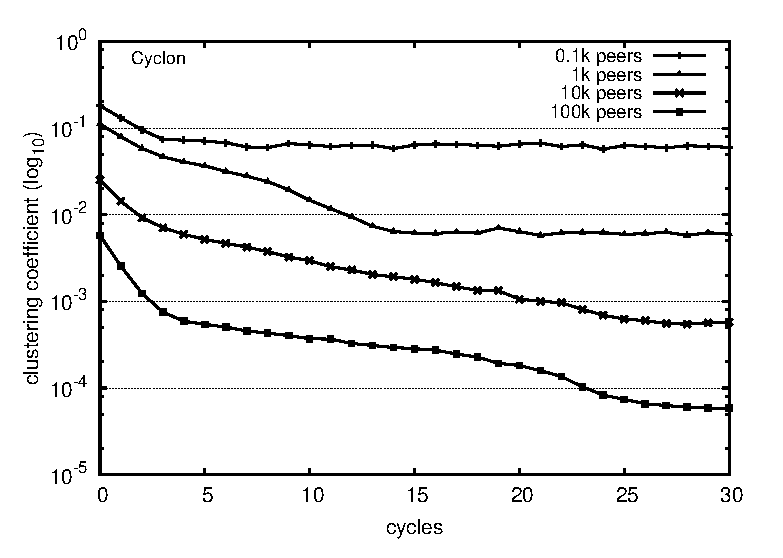
\includegraphics[width=0.47\textwidth]{img/spray/cycloncluster.eps}}
  \hspace{10pt}
  \subfloat[Coefficient d'agglomération de \SPRAY.]
  [Coefficient d'agglomération de \SPRAY.]
  {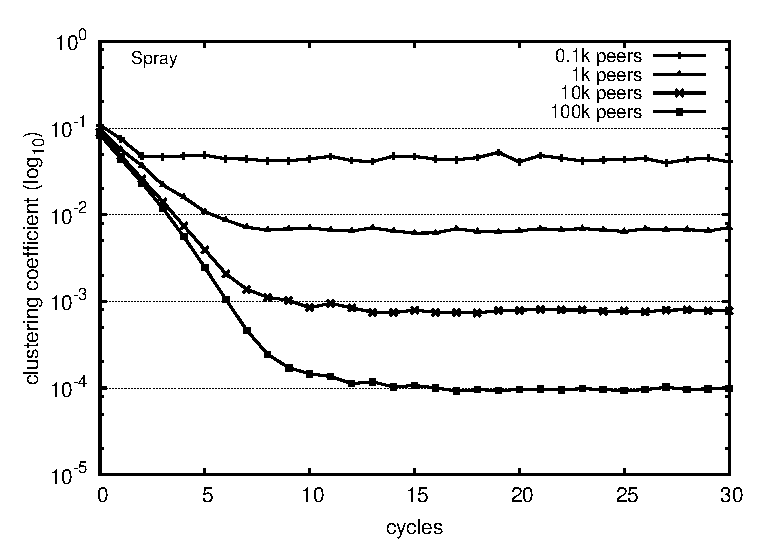
\includegraphics[width=0.47\textwidth]{img/spray/spraycluster.eps}}
  \caption{\label{net:fig:clustering}L'axe des abscisses marque le temps écoulé
    en nombre de cycles. L'axe des ordonnées note le coefficient d'agglomération
    sur une échelle logarithmique de base 10.}
\end{figure*}

\subsection{Coefficient d'agglomération}

\begin{asparadesc}
\item [Objectif:] Montrer comment l'adaptabilité influence le clustering et le
  temps de convergence.
\item [Description:] Le coefficient de clustering moyen $\overline{C}$ mesure la
  connexité du voisinage de chaque pair dans le réseau :
  \begin{equation}
    \overline{C} = {1\over |\mathcal{N}|}\sum\limits_{x\in\mathcal{N}}C_x
  \end{equation}
  où $C_x$ est le coefficient de clustering local du pair $p_x$. L'expérience
  implique 0.1k, 1k, 10k, et 100k pairs. Le représentant des approches à taille
  fixe est \CYCLON. Ce dernier est configuré de manière optimale pour 1k pairs
  ($\ln(1000)\approx 7$ voisins). Durant les échanges, les pairs utilisant
  \CYCLON mélangent 3 de leurs 7 voisins. Ainsi, les vues partielles de \CYCLON
  sont trop grandes pour 0.1k pairs, et trop petites pour 10k et 100k pairs.
\item [Résultat:] La figure~\ref{fig:spray:clustering} montre que \CYCLON
  démarre avec un coefficient de clustering plus bas que \SPRAY. Malgré cela,
  \SPRAY parvient à converger plus rapidement que \CYCLON. De plus, quand le
  nombre de pairs augmente dans le réseau, le temps de convergence de \CYCLON en
  souffre fortement. À l'opposé, \SPRAY converge très rapidement quel que soit
  la taille du réseau. La figure~\ref{fig:spray:clustering} montre aussi que les
  deux approches convergent vers un coefficient de clustering bas
  caractéristique des graphes aléatoires. Néanmoins, \CYCLON et \SPRAY
  n'atteignent pas les mêmes valeurs après convergence. À l'exception du cas où
  \CYCLON est configuré de manière optimale, les valeurs obtenus par \SPRAY sont
  soit au dessous (lorsque les vues de \CYCLON sont trop grandes) ou au dessus
  (lorsque les vues de \CYCLON sont trop petites). Globalement, cela montre que
  \SPRAY
  \begin{inparaenum}[(i)]
  \item converge vers un coefficient de clustering stable,
  \item qui reflète les besoins dû à la taille du réseau.
  \end{inparaenum}
  Cela a une influence sur l'équilibrage des charges et la robustesse par
  rapport aux allées et venues de pairs.    
\item [Explications:] \CYCLON commence avec un coefficient de clustering plus
  petit car lorsqu'un pair rejoint le réseau, un cheminement aléatoire est
  effectué afin d'en faire l'annonce. Ainsi, le réseau de départ est déjà
  légèrement équilibré au moment où la simulation commence les échanges de vue
  partielle. À l'opposé, un nouvel arrivant avec \SPRAY n'annonce son entrée
  qu'au voisinage de son contact. De ce fait, le réseau est fortement
  déséquilibré au départ de l'expérience, quelle que soit taille du
  réseau. Malgré cela, \CYCLON ne converge pas aussi vite que \SPRAY vers un
  coefficient stable. Cela est due à la taille fixe de sa vue partielle qui
  contraint la qualité des échanges. Le coefficient de clustering mesure la
  connexité du voisinage de chaque pair dans le réseau. Cela dépend donc de la
  taille de vue partielle qui, pour \CYCLON, est fixé lors de la configuration.
  Ainsi lorsque le nombre de pairs est multiplié par 10, le coefficient de
  clustering est divisé par 10. En revanche, les pairs utilisant \SPRAY ont une
  taille de vue partielle pouvant varier afin de refléter la taille du réseau.
  Ainsi, quand le réseau contient 1k pairs, les vues partielles s'adaptent à
  cette taille. Par conséquent, \SPRAY est très légèrement en dessous de \CYCLON
  dans ce scénario car la taille moyenne de vue partielle est de 7.4 pour ce
  premier contre 7 pour ce second. En étendant ce raisonnement aux autres
  tailles de réseau, cela explique pourquoi \SPRAY converge vers une valeur plus
  basse lorsque les vues partielles de \CYCLON sont trop grandes, et vers une
  valeur plus haute lorsque les vues partielles de \CYCLON sont trop petites.
\end{asparadesc}

\subsection{Plus court chemin moyen}

\begin{figure}
  \centering
  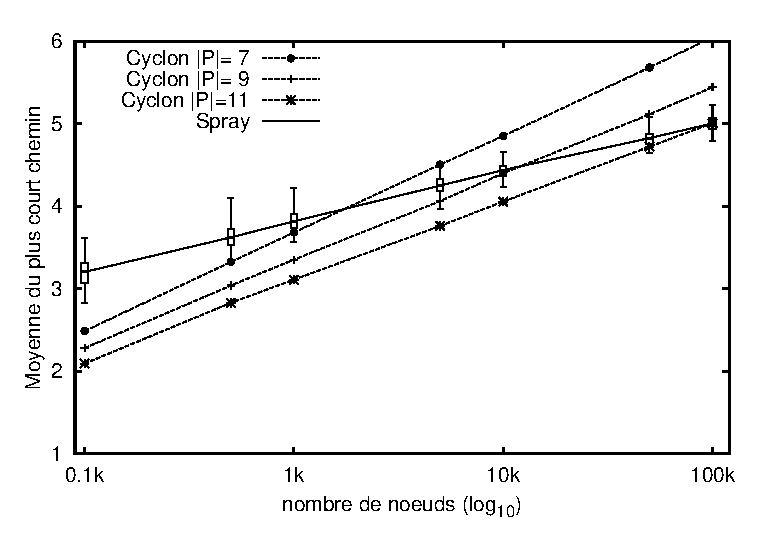
\includegraphics[width=.8\textwidth]{img/spray/avgpath.eps}
  \caption{\label{fig:spray:avgpath}The average shortest path length of \SPRAY
    and \CYCLON. The x-axis denotes the number of peers in the network on a
    $\log_{10}$ scale (from 100 to 100k peers) while the y-axis denotes the
    average shortest path length of the network.}
\end{figure}

\begin{asparadesc}
\item [Objectif:] Observer comment l'adaptabilité influence la taille du plus
  court chemin moyen, i.e., l'efficacité de la dissémination d'informations.
\item [Description:] La taille du plus petit chemin moyen est calculée en
  comptant le nombre de sauts (de voisin en voisin) d'un pair pour parvenir à
  tous les autres pairs. En d'autres termes, cette métrique indique le temps
  qu'une information, sous la forme d'un message, peut voyager et atteindre tous
  les pairs au moins une fois. Afin d'effectuer la moyenne, nous choisissons
  aléatoirement un sous-ensemble de pairs appartenant au réseau. Ce procédé est
  répété sur 100 exécutions afin d'éviter tous les effets de bord dus à
  l'indéterminisme des protocoles d'échantillonnages. Les expérimentations
  concernent \CYCLON configurés de façon optimale pour différentes tailles de
  réseau. Le \CYCLON avec une taille de vue partielle de 7 cible environ 1.1k
  pairs. Le \CYCLON avec une taille de vue partielle de 9 cible environ 8.1k
  pairs. Le \CYCLON avec une taille de vue partielle de 11 cible environ 60k
  pairs. Lors de toutes ces simulations, les mesures sont effectuées après
  convergence. Celles-ci sont faites lorsque la taille du réseau atteint 0.1k,
  0.5k, 1k, 5k, 10k, 50k, et 100k pairs. 
\item [Résultats:] La figure~\ref{fig:spray:avgpath} montre que \CYCLON et
  \SPRAY ont tous deux un chemin moyen relativement petit. Ainsi, les
  informations peuvent être disséminées à tous les membres du réseau très
  rapidement. La figure~\ref{fig:spray:avgpath} montre aussi que chaque
  exécution de \CYCLON prise séparément peut être divisée en trois phases.  Tout
  d'abord, la phase où les vues partielles de \CYCLON sont trop grandes
  dissémine l'information plus rapidement que \SPRAY. Lors les vues partielles
  sont optimales, \CYCLON et \SPRAY montrent des résultats similaires. Enfin,
  \SPRAY montre une meilleure efficacité lorsque les vues partielles de \CYCLON
  sont trop petites. Malgré tout, \SPRAY s'adapte mieux que \CYCLON à la taille
  du réseau car l'inclinaison de cette première est inférieure à n'importe
  quelle configuration de cette dernière.
\item [Explication:] Les mesures sont toutes effectuées après convergence,
  lorsque le réseau possède une topologie qui est proche d'un graphe aléatoire.
  Dans de tel graphe, le diamètre et la taille du plus court chemin moyen
  restent petits. La seconde observation concerne chacune des configurations de
  \CYCLON comparée à \SPRAY. Une taille de vue partielle surestimée pour \CYCLON
  est meilleure en terme de connexité entre pairs et résulte dans de plus courts
  chemins en moyenne. En revanche, dès que cette taille devient insuffisante
  pour le réseau, \SPRAY devient plus efficace car il possède de plus grandes
  vues partielles. Puisque \SPRAY suit toujours la taille optimale de vue
  partielle, il passe mieux à l'échelle en terme de taille réseau.
\end{asparadesc}

\subsection{Distribution des arcs entrants}

\begin{figure}
  \centering
  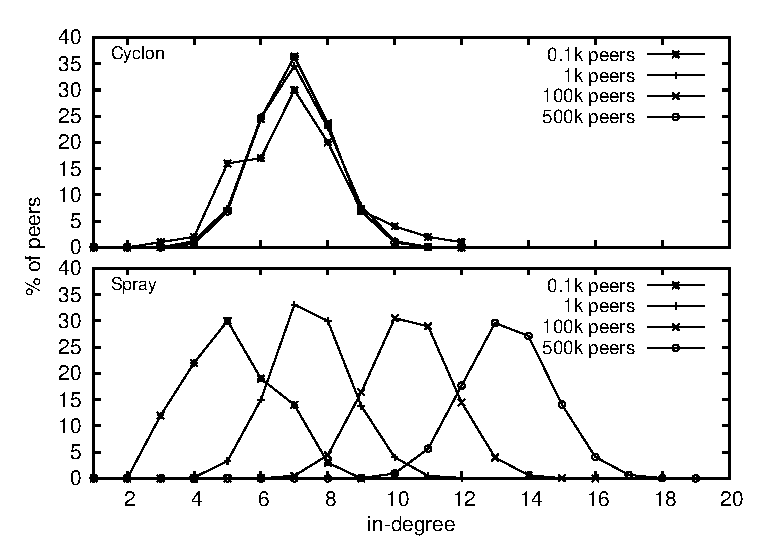
\includegraphics[width=.8\textwidth]{img/spray/histo.eps}
  \caption{\label{fig:spray:histo}The in-degree distribution of \CYCLON and
    \SPRAY. The x-axis denotes the in-degree in number of nodes while the
    y-axis indicates the percentage of peers with such in-degree. The top
    figure is dedicated to the runs concerning \CYCLON while the bottom figure
    concerns \SPRAY.}
\end{figure}

\begin{asparadesc}
\item [Objectif:] Montrer comment l'adaptabilité influence la distribution des
  connexions entrantes, i.e., la charge parmi les pairs.
\item [Description:] Les connexions entrantes d'un pair montre à quel point ce
  pair est représenté dans les vues partielles des autres pairs. La distribution
  des connexions entrantes permet de mettre en lumière l'existence de pairs avec
  une faible connexité, et les groupes fortement liés. Cela influence
  directement la robustesse du réseau. Dans cette expérimentation, \CYCLON est
  configuré avec une vue partielle contenant 7 voisins (optimal pour 1.1k
  pairs). Les mesures sont faites après convergence avec les tailles de réseau
  suivantes: 0.1k, 1k, 100k, 500k pairs.
\item [Résultat:] Le haut et le bas de la figure~\ref{fig:spray:histo} montrent
  la distribution des connexions entrantes pour \CYCLON et \SPRAY,
  respectivement. Nous observons que \CYCLON possède une distribution identique,
  quelle que soit la taille du réseau. Ainsi, la distribution d'un réseau de
  0.1k pairs est identique à celle de 500k pairs, avec une moyenne aux environs
  de 7 et un fort pic à cette valeur. À l'opposé, la distribution des connexions
  entrantes de \SPRAY suit la taille du réseau. La figure~\ref{fig:spray:histo}
  montre aussi que les pairs sont très concentrés autour des valeurs
  moyennes. Par exemple, lors de l'exécution du protocole \SPRAY avec 500k
  pairs, la moyenne est de 13.37 avec 88\% des pairs compris entre 12 et 14
  inclus. Cela signifie que la charge est très équilibrée parmi les
  pairs. Puisque chaque pair est aussi important que son voisin en terme de
  connectivité,le réseau est résistant aux défaillances.
\item [Explication:] Une fois configuré, \CYCLON doit gérer tous les réseaux,
  quelle que soit leur taille, avec une vue partielle dont la taille est
  constante. Proportionnelement, le nombre de fois qu'un pair est référencé dans
  les vues partielles ne change pas comparé à la taille réseau. En effet, le
  nombre d'arcs qu'un pair apporte lorsqu'il se connecte au réseau constitue
  autant d'arcs le ciblant après quelques protocoles d'échanges. Puisque la
  taille de la vue partielle est constante, le degré des connexions entrantes
  reste stable. En revanche, dans \SPRAY, chaque pair rejoignant le réseau
  augmente le nombre d'arcs dans le réseau. Ainsi, le degré de connexions
  entrantes de chaque pair grossit pour refléter la taille du réseau. Par
  conséquent, la distribution de \SPRAY se décale lentement vers de plus hautes
  valeurs lorsque la taille du réseau augmente. \SPRAY ne possède pas de pics
  sur les valeurs moyennes car celles-ci sont des valeurs qui tombent entre deux
  entiers. Par exemple, si la taille moyenne des vues partielles est 6.5, cela
  signifie que la moitié de celle-ci ont une taille de 6, et l'autre moitié une
  taille de 7. De tels réseaux sont robustes aux défaillances car aucun pair
  n'est plus important que son voisin en terme de connectivité. Ainsi, si un
  pair en particulier s'éteint, les pairs le référençant possèdent d'autres
  voisins avec qui communiquer pour continuer de disséminer les informations.
\end{asparadesc}

\subsection{Évolution du nombre d'arcs}

\begin{figure*}
  \centering
  \subfloat[Figure A][\label{fig:spray:churnA}The x-axis denotes the
  elapsed time in cycles. The upper graph y-axis shows the number of total
  connections in the overlay while the lower graph y-axis shows the variance
  $\sigma^2$ of the partial view sizes in the network.]{
    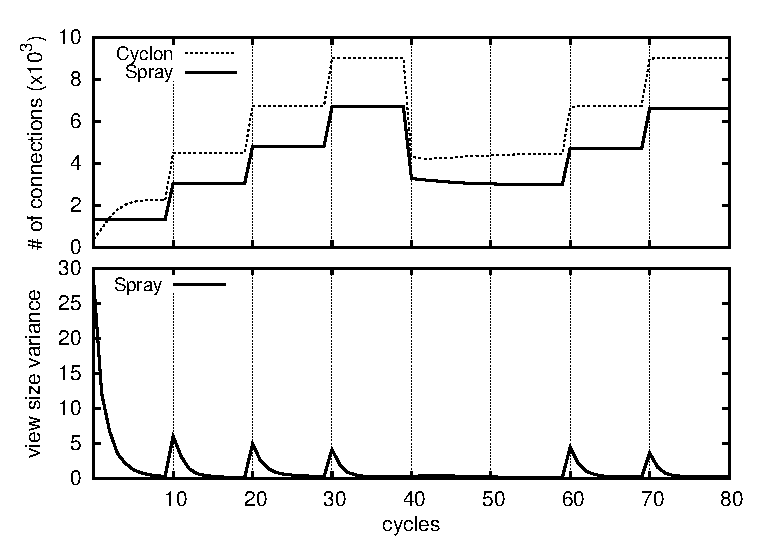
\includegraphics[width=0.47\textwidth]{img/spray/churn.eps}}
  \hspace{10pt}
  \subfloat[Figure B][\label{fig:spray:churnB}The x-axis denotes the
  elapsed time in cycles. The y-axis denotes the average partial view size.]{
    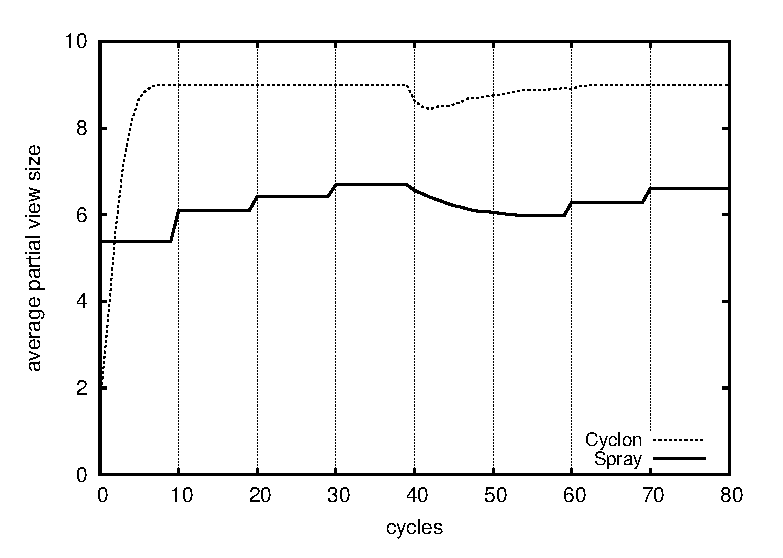
\includegraphics[width=0.47\textwidth]{img/spray/avgpv.eps}}
  \caption{\label{fig:spray:churn}\CYCLON (partial view size configured to 9)
    and \SPRAY in a dynamic network. 2.5k peers join the network at cycles $0$,
    $10$, $20$, and $30$. Then 5k peers leave at cycle $40$. Finally 2.5k peers
    join at cycles $60$ and $70$. The final network contains 10k members.}
\end{figure*}

\begin{asparadesc}
\item [Objectif:] Montrer comment l'influence de l'adaptabilité sur un réseau
  dont la taille varie au court du temps.
\item [Description:] Cette expérimentation se concentre sur un réseau dynamique
  dont les membres rejoignent et quittent le système lorsqu'ils le
  souhaitent. Les exécutions concernent les protocoles d'échantillonnage \CYCLON
  et \SPRAY. La configuration de \CYCLON cible un réseau de taille 8.1k
  pairs. Ainsi, les vues partielles sont trop grandes lors de cette simulation
  qui implique au maximum 1k pairs. Lors de la première moitié de la simulation,
  4 groupes successifs comportant 250 pairs rejoignent le réseau. L'intervalle
  de temps entre ces entrées groupées est de 10 cycles. Ainsi, le réseau
  initialement vide contient 1k pairs au bout de 40 cycles. Ensuite, la moitié
  des membres du réseau le quitte (500 pairs). Enfin, 2 groupes de 250 pairs
  rejoignent le réseau à nouveau faisant passer la taille de celui-ci à 1k
  pairs. Les mesures concernent
  \begin{inparaenum}[(i)]
  \item le nombre de connexions dans le réseau au cours des cycles,
  \item la variance de la taille des vues partielles au cours des cycles,
  \item la taille moyenne des vues partielles au cours du temps.
  \end{inparaenum}
\item [Résultat:] La figure~\ref{fig:spray:churn} montre les résultats de cette
  expérimentation. L'axe des abscisses représente les cycles (i.e. une mesure
  arbitraire de temps). La partie haute de la figure~\ref{fig:spray:churnA}
  montre le nombre de connections établies dans le réseau (échelle
  $\times 10^3$) tandis que la partie basse de la figure montre la variance de
  taille des vues partielles parmis les pairs. En ce qui concerne \SPRAY, nous
  observons qu'à chaque groupe rejoignant le réseau, le nombre de connections
  augmente afin de refléter cette augmentation. Ces observations concordent avec
  les mesures sur la variance. En effet, à chaque groupe rejoignant le réseau,
  la variance augmente soudainement. Ensuite, elle décroît exponentiellement et
  converge vers 0 en moins de 10 cycles. La variance est plus élevée lorsque la
  taille du réseau est basse. Par exemple, le premier groupe de 250 pairs
  conduit à la plus forte hausse de variance. Au $40^{ème}$ cycle, la moitié des
  pairs quittent le réseau. Approximativement la moitié des connections sont
  supprimées mais n'influent pas sur la variance. Les 10 cycles suivant montre
  une très faible diminution du nombre d'arcs. Enfin, de nouveaux groupes de
  pairs sont réintroduits dans le réseau et mène au même conclusions que
  précédemment. \CYCLON montre le même genre de comportement. Néanmoins, le
  nombre d'arcs est invariablement supérieurs à celui de \SPRAY (entre 1000 et
  2500 connexions supplémentaires). La figure~\ref{fig:spray:churnB} montre la
  taille moyenne des vues partielles de \SPRAY et de \CYCLON. Comme prévu,
  \CYCLON converge immédiatement vers la taille de vue partielle planifiée lors
  de sa configuration (9 voisins). À l'opposé, la taille de vue partielle
  moyenne de \SPRAY augmente logarithmiquement tandis que la taille du réseau
  augmente. Lorsque les départs de pairs surviennent au cycle 40, \CYCLON
  supprime les liens morts tout en remplissant les vues partielles afin
  d'atteindre la taille de vue partielle de sa configuration initiale. \SPRAY
  supprime seulement les arcs nécessaire afin de refléter la nouvelle taille
  réseau. À la fin de la simulation, les pairs utilisant \SPRAY ont une vue
  partielle contenant 6.6 voisins en moyenne (rappel: $\ln(1000)\approx 6.9$).
\item [Explication:] Puisque les vues partielles de \SPRAY s'adaptent à la
  taille du réseau, le nombre de connexions augmente lorsque des membres
  s'ajoute au réseau. Les pics de variance correspondent à la partie du
  protocole où les pairs rejoignent le réseau. Cette disparité provient du fait
  que les nouveaux arrivant commencent avec une petite vue partielle. Les pics
  sont plus petits lorsque le réseau est plus grand. En effet, les pairs étant
  présent avant que le nouveau groupe rejoigne le réseau ont eu quelques cycles
  d'échanges afin d'équilibrer leur vue partielle. Par conséquent, le poids des
  nouveaux arrivant est proportionnellement plus faible. Le départ des 500 pairs
  au cycle 40 ne perturbe pas la variance car ils sont effectués de manière
  aléatoire. Ainsi, aucun pair ne souffre plus qu'un autre des départs. La très
  petite décroissance du nombre d'arcs après les départs est due au fait que les
  pairs restant réalisent que les pairs sont injoignables seulement après
  quelques cycles. 
\end{asparadesc}

\subsection{Robustesse}

\begin{figure}
  \centering
  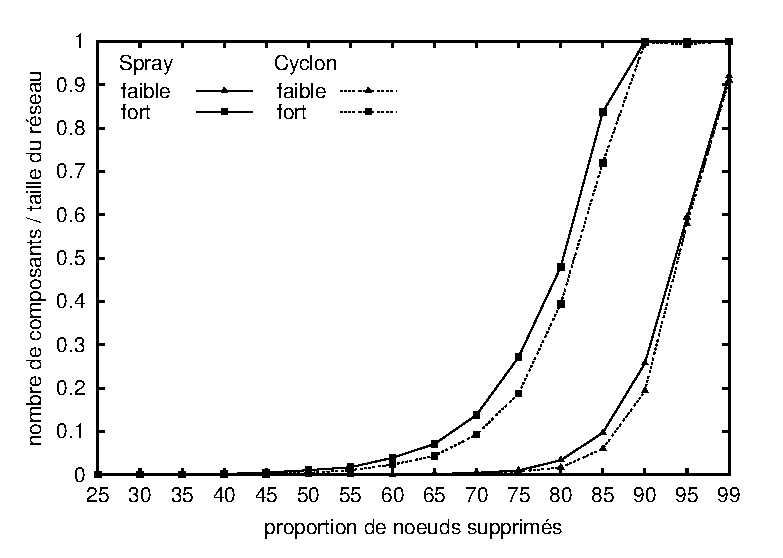
\includegraphics[width=.8\textwidth]{img/spray/resilience.eps}
  \caption{\label{fig:spray:resilience}Robustness of \CYCLON and \SPRAY to
    massive failures. The x-axis denotes the percentage of peers removed at once
    in a network containing 10k members. The y-axis denotes the number of
    components over the current network size (after the removals). The
    measurements concern the weak and strong components which basically means
    the number clusters in undirected or directed graph respectively.}
\end{figure}

\begin{asparadesc}
\item [Objectif:] Montrer que \SPRAY and \CYCLON sont tous deux robustes aux
  défaillances massives.
\item [Description:] Compter le nombre de composantes fortement connexes dans un
  réseau permet d'estimer la surface atteignable par les protocoles de
  dissémination d'informations. Par exemple, il y a deux composantes fortement
  connexes dans un réseau dont une partie peut atteindre l'autre sans que
  l'inverse soit vrai. Compter le nombre de composantes faiblement connexes dans
  une réseau permet d'estimer le moment où celui-ci n'est plus réparable. Un
  réseau est réparables si après quelques échanges de vues partielles, les
  informations peuvent être disséminées à tous les participants encore dans le
  réseau. \CYCLON est configuré pour obtenir des vues partielles contenant 9
  voisins. Le réseau compte 10k membres. Nous effectuons les suppressions de
  pairs après convergence des approches. Nous supprimons les pairs en une fois,
  allant de 25\% à 95\% par paliers de 5\% ce qui représente 16 exécutions par
  approche. La dernière mesure est effectuée à 99\% de suppressions. Les mesures
  sont effectuées immédiatement après les suppressions. Ces dernières concernent
  un pourcentage de pairs aléatoirement choisis parmi les 10k pairs.
\item [Résultat:] La figure~\ref{fig:spray:resilience} montre le ratio de
  composantes fortement/faiblement connexes du réseau après les suppressions de
  pairs. Tout d'abord, la figure montre que les deux protocoles
  d'échantillonnage de pairs, \SPRAY et \CYCLON, ne souffrent de comportement
  défaillant qu'après un haut pourcentage de suppressions, \CYCLON étant
  légèrement meilleur dans ce cas. La figure~\ref{fig:spray:resilience} montre
  que la dissémination d'informations (les composantes fortement connexes)
  commencent se dégrader lentement dès 45\%, et plus rapidement à
  70\%. Heureusement, la figure~\ref{fig:spray:resilience} nous montre aussi que
  ces approches sont capables de se réparer de ce clustering jusqu'à de haut
  taux de suppressions. En effet, les composantes faiblement connexes ne
  commencent à augmenter qu'à partir de 70\%, ce qui signifie que des parties du
  réseau sont complètement disjointes et donc, hors de toute possibilité de
  réparation.
\item [Explication:] Les protocoles d'échantillonnage de pairs \CYCLON et \SPRAY
  affichent de très similaires résultats car \CYCLON est configuré pour une
  taille de réseau de 10k pairs, tandis que \SPRAY s'ajuste automatiquement à
  cette taille de réseau. Par conséquent, leur nombre d'arcs est très
  proche. Ici, \CYCLON possède légèrement plus de connexions (car \SPRAY possède
  une part d'aléatoire) et aucun doublon dans les vues partielles (\SPRAY
  possède un faible taux de doublons,
  cf. Figure~\ref{fig:spray:duplicates}). Afin de mettre en dangers la
  dissémination d'information, il est nécessaire de supprimer un fort taux de
  pairs. En effet, chaque pair revêt grossièrement la même importance que son
  voisin. Ainsi, supprimer des pairs aléatoirement parmi ceux-ci n'affectent pas
  énormément le réseau en entier. Le réseau est capable de se réparer car les
  protocoles d'échantillonnage ne dépendent que d'arcs unidirectionnels pour
  fonctionner. Ainsi, s'il subsiste un lien entre deux composantes fortement
  connexes, les échanges de vues partielles permettent de réparer cela.
\end{asparadesc}

\subsection{Doublons}

\begin{figure}
  \centering
  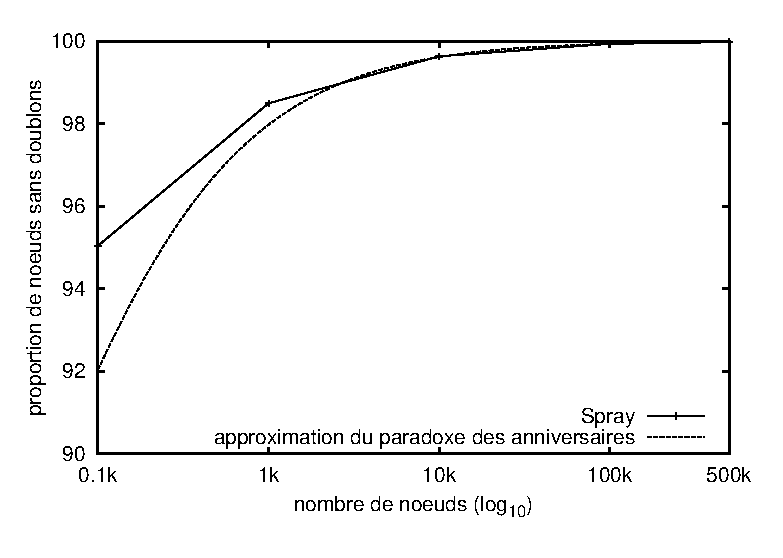
\includegraphics[width=.8\textwidth]{img/spray/duplicates.eps}
  \caption{\label{fig:duplicates}Duplicates in networks of different size: the
    $\log_{10}$-scaled x-axis denotes the network size while y-axis denotes the
    proportion of peers without any duplicates in their partial view.}
\end{figure}



% \begin{figure}
%   \centering 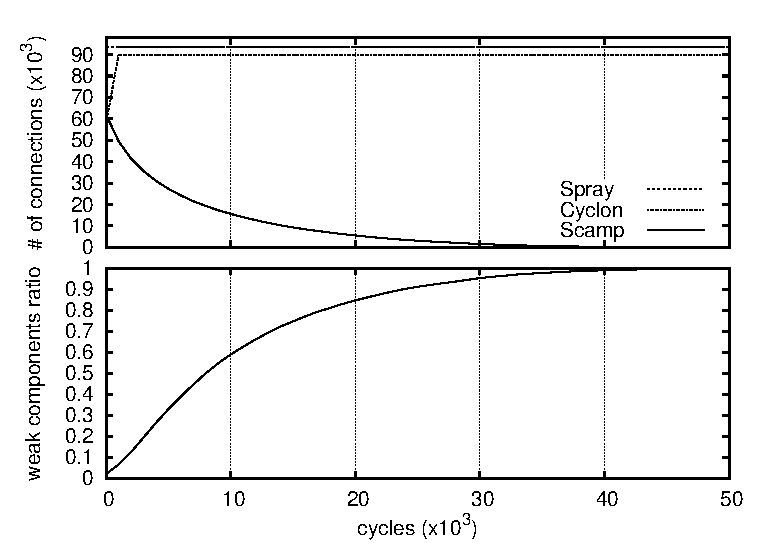
\includegraphics[width=.8\textwidth]{img/spray/degen.eps}
%   \caption{\label{fig:degeneration}\CYCLON, \SCAMP, and \SPRAY in network
%     subject to failures in the connection establishments. The x-axis denotes
%     the elapsed time in cycles ($10^3$-scaled). The y-axis of the top figure
%     denotes the global number of arcs ($10^3$-scaled). The y-axis of the bottom
%     figure denotes the ratio of weak components over the current network size.}
% \end{figure}

%%% Local Variables:
%%% mode: latex
%%% TeX-master: "../../paper"
%%% End:



\section{Cas d'utilisation : Dissémination de messages}
\label{net:sec:usecase}

La diffusion de messages d'un nœud à tous les autres est une fonctionnalité
courante des réseaux (\emph{broadcast}). La propagation épidémique
(\emph{gossip})~\cite{birman1999bimodal} constitue un moyen efficace de la
mettre en place. Sa dénomination provient de son fonctionnement : un nœud
choisit un sous-ensemble des membres du réseau et les ``contamine'' en leur
envoyant le message; les nœuds ``infectés'' en font de même; un nœud ayant déjà
envoyé le message ne le renvoie pas. Plus la taille du sous-ensemble choisi est
élevée, plus la probabilité selon laquelle le message parvient à tous les
membres du réseau augmente~\cite{erdos1959random}.

\begin{algorithm}
  
\small
\algrenewcommand{\algorithmiccomment}[1]{\hskip2em$\rhd$ #1}

\newcommand{\comment}[1]{\hfill $\rhd$ #1}

\newcommand{\LINEFOR}[2]{%
  \algorithmicfor\ {#1}\ \algorithmicdo\ {#2} %
  }

\newcommand{\LINEIFTHEN}[2]{%
  \algorithmicif\ {#1}\ \algorithmicthen\ {#2} %
  }

\newcommand{\INDSTATE}[1][1]{\State\hspace{\algorithmicindent}}

\begin{algorithmic}[1]
  \Function{broadcast}{$m$} \comment{$m$: \emph{message to send}}
  \State \textbf{let} $chosen \leftarrow getPeers(P,\, \DARKBLUE{fanout})$;
  \For{(\DARKBLUE{$n \in chosen$})}
  \State \textsc{sendTo}($n$, 'broadcast', $m$);
  \EndFor
  \EndFunction

  \Statex

  \Function{onBroadcast}{$m$} \comment{$m$: \emph{received message}}
  \If {($\DARKBLUE{\neg\textsc{alreadyReceived}(m)}$)}
  \State \textsc{broadcast}($m$);
  \EndIf
  \EndFunction
\end{algorithmic}

  \caption[Algorithme de dissémination de
  messages]{\label{net:algo:broadcast}Algorithme de dissémination de messages.}
\end{algorithm}


L'algorithme~\ref{net:algo:broadcast} montre les quelques instructions composant
la dissémination épidémique de messages. L'épanouissement (\emph{fanout})
désigne le nombre de voisins auxquels le message va être envoyé. La fonction
\textsc{getPeers} renvoie autant de nœuds distincts. Dans le cadre d'approches
fournissant une vue partielle de taille constante, cette variable
d'épanouissement est elle aussi constante, et configurée à l'avance. Pour que
les chemins employés lors de la dissémination soient eux aussi aléatoires malgré
la fréquence beaucoup plus faible des échanges du protocole d'échantillonnage,
la taille de la vue est nettement surestimée~\cite{frey2009heterogeneous}. Par
exemple, une vue partielle contient 30 arcs, mais seulement 6 sont employés à
chaque dissémination. Dans le cadre de \SPRAY, nous augmentons les tailles des
vues partielles fournies : lors de l'entrée dans le réseau, un nœud n'ajoute
plus qu'une seule référence au contact mais $c$ doublons; les vues partielles
tendent vers $c\cdot\ln(|\mathcal{N}|)$~\cite{ganesh2003peer}; un nœud détectant
un départ ou une panne ajuste la probabilité de supprimer un arc à
$c \div (|P|+occ)$. La variable d'épanouissement est configurée comme étant une
fraction de la vue partielle. Ainsi l'épanouissement peut s'ajuster
automatiquement pour suivre une progression logarithmique :
$\ln(|\mathcal{N}|)+x$, où $x$ est un entier positif.

La suite met en évidence l'avantage apporté par une variable d'épanouissement
s'ajustant à la taille du réseau. En particulier, nous mesurerons le taux de
réception totale des messages par les membres du réseau. Si au moins un membre
ne reçoit pas le message, alors la réception totale à échouée. Le taux mesuré
est le nombre de messages ayant été reçus par tout les membres sur le nombre de
messages ayant été envoyés.

\paragraph{Objectif :} Montrer les bénéfices apportées au mécanisme de
dissémination par un protocole adaptatif d'échantillonnage.

\paragraph{Description :} L'application considérée cible approximativement 100
nœuds. Les vues partielles fournies par \CYCLON sont configurées pour contenir
30 voisins ($6 \cdot \ln(100) \approx 6 \cdot 5 = 30$). Nous considérons 2
configurations pour l'épanouissement : $\ln(100)+1 \approx 6$ et
$\ln(100)+3 \approx 8$. Ces configurations garantissent une forte probabilité de
réception des messages lorsque le réseau contient 100 nœuds ou moins. De même,
nous configurons \SPRAY pour qu'il fournisse des vues partielles 6 fois plus
peuplés qu'à la normale. La variable d'épanouissement est configurée pour
choisir 1 sixième de la vue, soit $\ln(|\mathcal{N}|)+1$ et
$\ln(|\mathcal{N}|)+3$.  Les deux protocoles d'échantillonnage aléatoire
possèdent donc les même configurations pour un réseau de 100 nœuds. La taille
des réseaux considérés grandit de 0.1k à 2k nœuds. Nous mesurons à chaque cycle
la fraction, sur 1k messages, parvenant à l'intégralité des membres du réseau.

\begin{figure}
  \begin{center}
    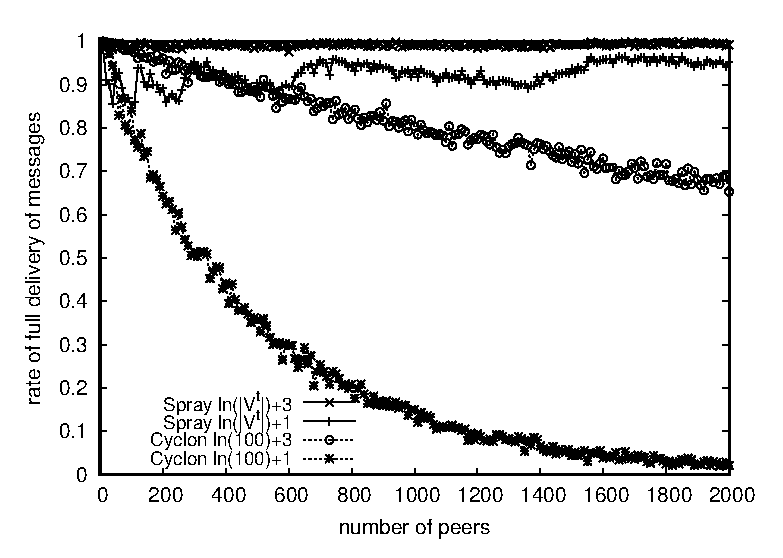
\includegraphics[width=.8\textwidth]{img/spray/hardrate.eps}
    \caption[Taux de réception des messages comparé à la taille du
    réseau.]{\label{net:fig:hardrate} Taux de réception des messages comparé à
      la taille du réseau. L'axe des abscisses montre la taille du réseau en
      nombre de nœuds. L'axe des ordonnées montre le taux de réception total
      mesuré sur 1k messages.}
  \end{center}
\end{figure}

\paragraph{Résultat :} La figure~\ref{net:fig:hardrate} présente les résultats
de cette simulation. Tout d'abord, nous observons que le taux de réception des
messages avec \CYCLON souffre d'une constante décroissance. De moins en moins de
messages parviennent à l'ensemble des nœuds lorsque le réseau s'agrandit. La
configuration dont la variable d'épanouissement est la plus élevée fournie de
meilleurs résultats. En revanche, le taux de réception des messages de \SPRAY
reste stable bien que nous puissions observer la présence de petits sauts dans
les valeurs mesurées. Un épanouissement initialisé à $\ln(|\mathcal{N}|)+1$
conduit à un taux aux environs de 90\%. Un épanouissement initialisé à
$\ln(|\mathcal{N}|)+3$ conduit à un taux proche de 100\%. Globalement, le
mécanisme de dissémination épidémique présenté profite bien de la nature
adaptative de \SPRAY. Cela lui permet de s'ajuster aux besoins d'un réseau dont
la taille fluctue au cours du temps.

\paragraph{Explication :} Le seuil précis de connexité d'un graphe aléatoire est
$\Theta(|\mathcal{N}|\ln(|\mathcal{N}|))$ arcs. Pour la dissémination de
messages cela signifie que, avec des vues partielles suffisamment grandes et
peuplées d'arcs vers des nœuds suffisamment aléatoires, un épanouissement fixé à
$\ln(|\mathcal{N}|)$ conduit à un taux de réception aux environs de 50\%. À ce
stade, incrémenter cette variable augmente drastiquement le taux de
réception. Cependant, la contribution de chaque incrémentation diminue petit à
petit par rapport à l'incrémentation précédente. Le mécanisme de dissémination
construit au dessus de \CYCLON possède un épanouissement constant, configuré
pour une taille spécifique du réseau. Tant que la taille du réseau est
inférieure ou égale à la taille ciblée, le taux de réception demeure élevé. En
revanche, une fois cette taille dépassée, le taux de réception chute très
rapidement. \SPRAY donne la possibilité au mécanisme de dissémination d'ajuster
sa variable d'épanouissement à la taille du réseau. Ainsi, le taux de réception
des messages reste stable, même lorsque le réseau s'agrandit. Les petits sauts
mesurées sont dûs au fait que les valeurs manipulées localement par chaque nœuds
sont des entiers. Le bond correspond donc à une valeur arrondie augmentant
suffisamment pour être incrémentée.

%%%%%%

\paragraph{Objectif :} Montrer comment le taux de réception des messages se
comporte lors d'un pique de population, i.e., une augmentation massive de la
taille du réseau suivie peut après d'une diminution.

\paragraph{Description :} Nous configurons \SPRAY et \CYCLON de la même manière
que pour la précédente simulation. Pour \CYCLON, les vues partielles sont
initialisées à 30 voisins avec deux valeurs pour l'épanouissement : $\ln(100)+1$
et $\ln(100)+3$. Pour \SPRAY, les vues partielles s'ajustent automatiquement à
$6\cdot \ln(|\mathcal{N}|)$ et les valeurs d'épanouissement s'ajustent
automatiquement à $\ln(|\mathcal{N}|)+1$ et $\ln(|\mathcal{N}|)+3$. La
simulation commence avec 0.1k nœuds. Le réseau atteint rapidement 10k nœuds
pendant le pique de popularité. Enfin il redescend à 3k nœuds. Dans cette
simulation, nous mesurons le taux de réception total des messages sur 0.1k
messages.

\begin{figure}
  \begin{center}
    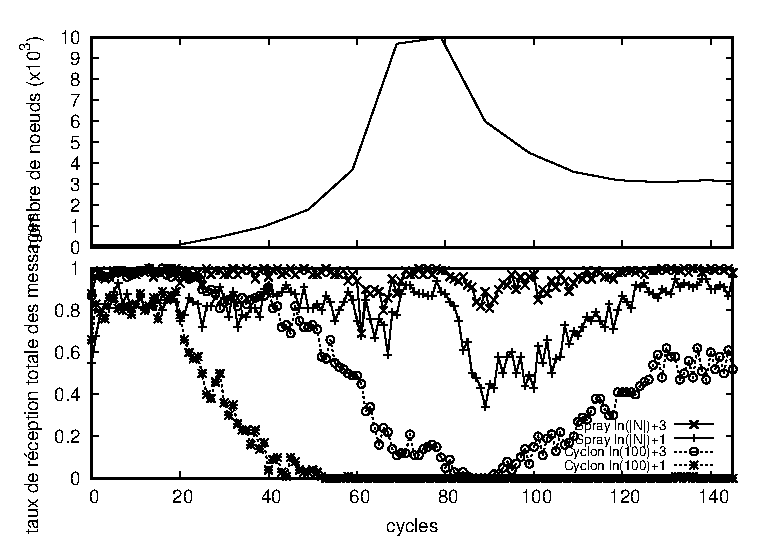
\includegraphics[width=.8\textwidth]{img/spray/peak.eps}
    \caption[Taux de réception des messages lors d'un pique de
    population]{\label{net:fig:peak} Taux de réception des messages lors d'un
      pique d'entrée dans le réseau. L'axe des abscisses montre le temps en
      nombre de cycles. L'axe des ordonnées de la partie haute montre le nombre
      de nœuds présent dans le réseau. L'axe des ordonnées de la partie basse
      montre le taux de réception des messages sur 0.1k messages.}
  \end{center}
\end{figure}

\paragraph{Résultat :} La figure~\ref{net:fig:peak} montre les résultats de
cette simulation. Tout comme lors de la simulation précédente, l'utilisation de
\CYCLON et d'une variable d'épanouissement prédéfinie fonctionne jusqu'à ce que
la taille du réseau excède la taille prévue. Pendant le pique d'entrée dans le
réseau, le taux de réception chute très rapidement. À l'inverse, le mécanisme de
dissémination construit avec \LSEQ ajuste automatiquement sa variable
d'épanouissement à la taille du réseau. Ainsi, le système ne souffre pas de
sévère baisse du taux de réception lors du pique d'entrée. Cependant, lors du
départ massif de certains membres, le taux de réception chute. Cela est
particulièrement vrai pour la configuration de \SPRAY avec un épanouissement
plus modeste de $\ln(|\mathcal{N}|)+1$. Globalement, le mécanisme de
dissémination se comporte mieux avec \SPRAY et devient résilient aux
fluctuations rapides de la taille des réseaux.

\paragraph{Explication :} La variable d'épanouissement des configurations
impliquant \CYCLON est constante. Ainsi, lorsque la taille du réseau dépasse la
taille prévue, le taux de réception chute drastiquement. À l'opposé, la
variable d'épanouissement des configurations basés sur \SPRAY suit les
évolutions du réseau. Le taux de réception reste stable lors d'augmentations
rapides de la taille du réseau. Cependant, à la fois \CYCLON et \SPRAY détectent
les nœuds partis lors de la phase d'échange de vues partielles. Les arcs
obsolètes sont malgré tout utilisés dans la dissémination. Par conséquent, un
plus grand nombre de messages à tendance à se perdre. Petit à petit, les arcs
obsolètes disparaissent des vues partielles. Le taux de réception des messages
recouvre sa valeur attendue.

%%% Local Variables:
%%% mode: latex
%%% TeX-master: "../../paper"
%%% End:



\section{Conclusion}
\label{net:sec:conclusion}

Dans ce chapitre, nous avons présenté \SPRAY, un protocole d'échantillonnage
aléatoire de pairs s'ajustant automatiquement aux fluctuations de la taille du
réseau. Chaque nœud d'un réseau de taille $|\mathcal{N}|$ se voit attribuer une
vue partielle du réseau de taille $\ln |\mathcal{N}|$ avec laquelle il peut
communiquer. Périodiquement, les nœuds échangent une partie de leur vue
partielle avec leur voisin le plus âgé. Bien que l'identité des nœuds ne se
propagent que de voisin à voisin, le réseau converge vers une topologie dont les
propriétés sont stables en très peu de temps. La topologie résultant de ces
mélanges de voisinages possède des propriétés proches des graphes
aléatoires. Par exemple, le réseau est tolérant aux pannes et les messages se
propagent efficacement.

Un développeur peut utiliser \SPRAY afin que le trafic généré suive les
variations du réseau, et ce, sans configuration préalable de sa part. Le
chapitre~\ref{editor:chap:crate} montre un exemple d'utilisation de \SPRAY dans
le contexte de l'édition collaborative temps réel dans les navigateurs Web.  Ce
contexte est propice à son utilisation car l'établissement de connexion d'un
navigateur à l'autre s'avère coûteux. Par conséquent, conserver un nombre
logarithmique de connexions s'établissant précautionneusement de proche en
proche constitue un avantage. De plus, le Web favorisant les échanges et la
propagation d'idées, un éditeur Web doit être capable de faire face aux pics
soudains de popularité.



%%% Local Variables:
%%% mode: latex
%%% TeX-master: "../../paper"
%%% End:


\chapter{Un éditeur collaboratif temps-réel dans les navigateurs}
\label{editor:chap:crate}
\minitoc

\TODO{introduction}


\section{État de l'art}

Les éditeurs collaboratifs répartis autorisant l'édition temps réel dans les
navigateurs web sont centralisés. Entre autres, les éditeurs tels que Google
Docs~\cite{googledocs} ou Etherpad~\cite{etherpad} ont rendu l'édition
collaborative aisée pour les millions d'utilisateurs à travers le monde.

\begin{figure}
  \begin{center}
    \begin{tikzpicture}[scale=1.2]
  
  \newcommand\X{40pt}
  \newcommand\Y{-50pt}
  
  \draw[->, very thick, color=darkblue](-2.5-2*\X, 5+1*\Y)--(-2.5-1.5*\X, -10pt);
  \draw[<-, dashed](2.5-2*\X, 5+1*\Y)--(2.5-1.5*\X, -10pt);

  \draw[->, dashed](-2.5-1*\X, 5+1*\Y)--(-2.5-1*\X, -10pt);
  \draw[<-, very thick, color=darkblue](2.5-1*\X, 5+1*\Y)--(2.5-1*\X, -10pt);

  \draw[->, dashed](-2.5+0*\X, 5+1*\Y)--(-2.5+0*\X, -10pt);
  \draw[<-, very thick, color=darkblue](2.5+0*\X, 5+1*\Y)--(2.5+0*\X, -10pt);
    
  \draw[->, dashed](-2.5+1*\X, 10+1*\Y)--(-2.5+0.5*\X, -10pt);
  \draw[<-, very thick, color=darkblue](2.5+1*\X, 10+1*\Y)--(2.5+0.5*\X, -10pt);


  \draw[fill=white](-0.5*\X, 0*\Y) node{Service provider's document server}
  +(-70pt,-10pt )rectangle+(70pt,10pt);

  \draw[fill=white](-2*\X, 1*\Y) node{$e_1$}
  +(5pt, 5pt) rectangle +(-5pt, -5pt) rectangle +(5pt, 5pt);
  \draw[fill=white](-1*\X, 1*\Y) node{$e_2$}
  +(5pt, 5pt) rectangle +(-5pt, -5pt) rectangle +(5pt, 5pt);
  \draw[fill=white]( 0*\X, 1*\Y) node{$e_3$}
  +(5pt, 5pt) rectangle +(-5pt, -5pt) rectangle +(5pt, 5pt);



  \draw[->,dashed](-2.5+1.5*\X, 5+2*\Y)--(-2.5+1.5*\X, -10+1*\Y);
  \draw[<-,very thick, color=darkblue]( 2.5+1.5*\X, 5+2*\Y)--( 2.5+1.5*\X, -10+1*\Y);

  \draw[->,dashed](-2.5+2.5*\X, 5+2*\Y)--(-2.5+2.5*\X, -10+1*\Y);
  \draw[<-,very thick, color=darkblue]( 2.5+2.5*\X, 5+2*\Y)--( 2.5+2.5*\X, -10+1*\Y);

  \draw[->,dashed](-2.5+3.5*\X, 5+2*\Y)--(-2.5+3.5*\X, -10+1*\Y);
  \draw[<-,very thick, color=darkblue]( 2.5+3.5*\X, 5+2*\Y)--( 2.5+3.5*\X, -10+1*\Y);

  \draw[->,dashed](-2.5+4.5*\X, 5+2*\Y)--(-2.5+4.5*\X, -10+1*\Y);
  \draw[<-,very thick, color=darkblue]( 2.5+4.5*\X, 5+2*\Y)--( 2.5+4.5*\X, -10+1*\Y);

  \draw[fill=white](3*\X, 1*\Y) node{Service provider's transmission server}
  +(-100pt,-10pt )rectangle+(100pt,10pt);

  \draw[fill=white]( 1.5*\X, 2*\Y) node{$e_4$}
  +(5pt, 5pt) rectangle +(-5pt, -5pt) rectangle +(5pt, 5pt);
  \draw[fill=white]( 2.5*\X, 2*\Y) node{$e_5$}
  +(5pt, 5pt) rectangle +(-5pt, -5pt) rectangle +(5pt, 5pt);
  \draw[fill=white]( 3.5*\X, 2*\Y) node{$e_6$}
  +(5pt, 5pt) rectangle +(-5pt, -5pt) rectangle +(5pt, 5pt);
  \draw[fill=white]( 4.5*\X, 2*\Y) node{$e_7$}
  +(5pt, 5pt) rectangle +(-5pt, -5pt) rectangle +(5pt, 5pt);

\end{tikzpicture}
    \caption{\label{editor:fig:serviceprovider} Les transmissions aux clients
      connectés et les transformations d'opérations sont à la charge du 
      fournisseur de services.}
  \end{center}
\end{figure}

La figure~\ref{editor:fig:serviceprovider} montre le fonctionnement de ces
éditeurs. Un serveur central possède le document. Les participants se connectent
à ce serveur (i.e. $e_1$, $e_2$, et $e_3$) ou à un serveur associé (i.e. $e_4$,
$e_5$, $e_6$, $e_7$) mis à disposition de manière élastique afin d'alléger la
charge de diffusion des messages du premier. Lorsque le collaborateur $e_1$
effectue une action telle que l'insertion d'un caractère, l'opération est émise
au serveur possédant le document. Celui-ci, fonctionnant avec une approche de
transformés opérationnels, transforme l'opération reçue vis-à-vis de toutes
celles que l'utilisateur n'avait pas encore reçu lors de la création de son
opération. La transformation s'avère toutefois moins coûteuse puisque seul le
serveur doit l'effectuer. En particulier, le vecteur de contexte transporté dans
les messages des approches OT décentralisées n'existe pas dans les versions
centralisée puisque seule importe la paire de versions de l'utilisateur et du
serveur. En revanche, le serveur est en charge de toutes les transformations. De
plus, il doit diffuser l'ensemble des changements aux participants. Le
fournisseur de service prend en charge la presque intégralité du coût de la
session d'édition. Pour les utilisateurs, se posent toujours les problèmes de
confidentialité : Le fournisseur de service voit les documents et peut en
utiliser le contenu à ses propres fins. Pire encore, la propriété du document
doit bien souvent être accordée au fournisseur de service. À cela s'ajoute le
problème du point individuel de défaillance : Lorsque le serveur hébergeant le
document tombe en panne, le document n'est plus accessible.

Malgré tous ces défauts, ces approches centralisées sont les plus populaires.
Jusqu'à présent, aucun éditeur décentralisé dans le navigateur web n'avait été
déployé. La récente technologie WebRTC permet d'établir des canaux de
communication d'un navigateur à l'autre. En d'autres termes, les applications
réellement décentralisée aussi facile d'accès que les applications web du Nuage
deviennent possibles.

\paragraph{WebRTC~\cite{webrtc}.} Acronyme de \emph{Web Real-Time
  Communication}.  Cette technologie permet l'établissement de canaux de
communication d'un navigateur web à l'autre, et ce, même en présence de
configurations réseaux complexes impliquant firewall, proxy, ou NAT (Network
Address Translation). Toutefois, WebRTC ne gère ni l'adressage, ni le routage.
Établir une connexion WebRTC requière une négociation où le nœud d'origine et le
nœud de réception s'envoient mutuellement des moyens d'accès distants dans
l'ordre définit du plus aisé au plus ardu. Par exemple, les échanges vont
d'abord concerner la boucle locale (\emph{localhost}), puis le réseau local
(e.g. $192.168.255.255$), puis l'internet\ldots Aussitôt que la négociation
s'achève avec succès, un canal de communication bidirectionnel est établi. Les
nœuds peuvent alors communiquer entre eux.

\begin{figure*}
  \begin{center}
    \subfloat[Figure A][\label{editor:fig:webrtcA}
    $e_1$ se connecte à $e_2$ via un médiateur.
    1: $e_1$ crée ses offres;
    2: $e_2$ récupère ces offres;
    3: $e_2$ crée ses offres en réponse;
    4: $e_1$: reçoit les offres et établit une connexion bidirectionnelle avec
    $e_2$. $e_3$ en fait de même avec $e_2$.
    La figure~\ref{editor:fig:webrtcB} décrit le réseau en résultant.]{
      
\begin{tikzpicture}[scale=1.2]

\newcommand\X{40pt};
\newcommand\Y{15pt};

\draw( 1.7*\X, 0); %% spacing
\draw(-1.7*\X, 0); %% spacing

\draw[fill=white,very thick, draw=darkblue](0*\X, 0*\Y) 
node{\DARKBLUE{\emph{serveur de signalement}}} +(-45pt,-5pt) rectangle +(45pt,5pt);

\small
\draw[->,dashed, very thick](-5 -1*\X, 5-2*\Y) --
node[anchor=east]{1} (-20pt,-5pt);
\draw[->,dashed, very thick]( 5 -1*\X, 5-2*\Y) --
node[anchor=west]{4} (-10pt,-5pt);

\draw[->,dashed, very thick](-5pt,  5-3*\Y) --
node[anchor=east]{2}(-5pt,-5pt);
\draw[->,dashed, very thick](5pt , 5-3*\Y) --
node[anchor=west]{3} (5pt,-5pt);


\draw[fill=white, very thick]
(-1*\X,-2*\Y) node{$n_1$} +(-5pt,-5pt) rectangle +(5pt,5pt);
\draw[fill=white, very thick]
(0*\X, -3*\Y) node{$n_2$} +(-5pt,-5pt) rectangle +(5pt,5pt);
\draw[fill=white] (1*\X, -2*\Y) node{$n_3$} +(-5pt,-5pt) rectangle +(5pt,5pt);

\end{tikzpicture}

% \begin{tikzpicture}
% \matrix (m) [matrix of math nodes,row sep=4em,column sep=4em] {
% \node(ss)[draw]{signaling}; & \node(p3)[draw]{p3}; \\
% \node(p1)[draw]{p1}; & \node(p2)[draw]{p2}; \\
% };
% \path[->]
%   (p2) edge[dashed] node[fill=white]{1:emit} (ss)
%   (p3) edge[dashed] node[fill=white,bend left]{2:pull} (ss)
%   (p3) edge[dashed, bend right] node[fill=white]{3:accept} (ss)
%   (p2) edge[dashed,bend left] node[fill=white]{4:pull} (ss)
%   (p3) edge[<->,thick] node[fill=white,right]{5:connected} (p2);
% \end{tikzpicture}}
    \hspace{5pt}
    \subfloat[Figure B][\label{editor:fig:webrtcB}
    $e_1$ se connecte à $e_3$ en utilisant $e_2$ comme médiateur.
    1: $e_1$ envoie ses offres à $e_2$;
    2: $e_2$ redirige les offres à $e_3$;
    3: $e_3$ envoie ses offres en réponse à $e_2$;
    4: $e_2$ redirige les offres vers $e_1$ qui se connecte à $e_3$.]{
      
\begin{tikzpicture}[scale=1.2]

\newcommand\X{40pt};
\newcommand\Y{15pt};

\draw(1.7*\X, 0); %% spacing
\draw(-1.7*\X, 0); %% spacing

\draw[fill=white](0*\X, 0*\Y)
node{\emph{serveur de signalement}} +(-45pt,-5pt) rectangle +(45pt,5pt);

\small
\draw[<->, very thick](5-1*\X,-2*\Y)--
node[anchor=south]{1$\rightarrow$}
node[anchor=north]{$\leftarrow$4}(-5pt,-3*\Y);
\draw[<->, very thick](5pt,-3*\Y)--
node[anchor=south]{2$\rightarrow$}
node[anchor=north]{$\leftarrow$3}(-5+1*\X,-2*\Y);

\draw[fill=white, very thick]
(-1*\X,-2*\Y) node{$n_1$} +(-5pt,-5pt) rectangle +(5pt,5pt);
\draw[fill=white, very thick, draw=darkblue]
(0*\X, -3*\Y) node{\DARKBLUE{$n_2$}} +(-5pt,-5pt) rectangle +(5pt,5pt);
\draw[fill=white, very thick]
(1*\X, -2*\Y) node{$n_3$} +(-5pt,-5pt) rectangle +(5pt,5pt);

\end{tikzpicture}

% \begin{tikzpicture}
% \matrix (m) [matrix of math nodes,row sep=4em,column sep=4em] {
% \node(ss)[draw]{signaling}; & \node(p3)[draw]{p3}; \\
% \node(p1)[draw]{p1}; & \node(p2)[draw]{p2}; \\
% };
% \path[->]
%   (p1) edge[dashed,bend left] node[fill=white]{1:emit} (p2)
%   (p2) edge[dashed,bend left] node[fill=white,left]{2:emit/p1} (p3)
%   (p3) edge[dashed,bend left] node[fill=white,right]{3:accept/p1} (p2)
%   (p2) edge[dashed,bend left] node[fill=white]{4:accept} (p1)
%   (p1) edge[<->,thick] (p2)
% %  (p1) edge[<->,thick,bend left] (p3)
%   (p2) edge[<->,thick]  (p3);

% \end{tikzpicture}}
    \hspace{5pt}
    \subfloat[Figure C][\label{editor:fig:webrtcC}
    Le réseau superposé : Un réseau complètement connecté composé de 3 membres.]{
      
\begin{tikzpicture}[scale=1.2]

\newcommand\X{40pt};
\newcommand\Y{15pt};

\draw(1.7*\X, 0); %% spacing
\draw(-1.7*\X, 0); %% spacing

\draw[fill=white](0*\X, 0*\Y)
node{\emph{serveur de signalement}} +(-45pt,-5pt) rectangle +(45pt,5pt);

\small
\draw[<->](5-1*\X,-2*\Y)--(-5pt,-3*\Y);
\draw[<->](5pt,-3*\Y)--(-5+1*\X,-2*\Y);
\draw[<->, very thick, color=darkblue]
(5 - 1*\X, 2.5 -2*\Y)--(-5+1*\X, 2.5 -2*\Y);

\draw[fill=white]
(-1*\X,-2*\Y) node{$n_1$} +(-5pt,-5pt) rectangle +(5pt,5pt);
\draw[fill=white]
(0*\X, -3*\Y) node{$n_2$} +(-5pt,-5pt) rectangle +(5pt,5pt);
\draw[fill=white]
(1*\X, -2*\Y) node{$n_3$} +(-5pt,-5pt) rectangle +(5pt,5pt);

\end{tikzpicture}


% \begin{tikzpicture}
% \matrix (m) [matrix of math nodes,row sep=4em,column sep=4em] {
% \node(ss)[draw]{signaling}; & \node(p3)[draw]{p3}; \\
% \node(p1)[draw]{p1}; & \node(p2)[draw]{p2}; \\
% };
% \path[->]
%   (p1) edge[<->,thick] (p2)
%   (p1) edge[<->,thick] (p3)
%   (p2) edge[<->,thick]  (p3);
% \end{tikzpicture}}
    \caption{\label{fig:webrtc}Créer un réseau superposé au dessus de WebRTC.}
  \end{center}
\end{figure*}

\noindent Pour établir une connexion, les navigateurs s'échangent des offres et
acquittements via un médiateur commun (e.g. mails, services dédiés de
signalement, connexions WebRTC connues, etc.). Dans la figure~\ref{editor:fig:webrtcA},
$e_1$ souhaite se connecter à $e_2$. Par conséquent, $e_1$ envoie ses offres au
service de signalement connu. Le nœud $e_2$ récupère l'offre et envoie ses
propres offres en réponse au service de signalement. Enfin, $e_1$ récupère les
offres de $e_2$ et établit une connexion bidirectionnelle avec $e_2$. De manière
identique, $e_3$ établit une connexion avec $e_2$. Désormais, le nœud $e_1$ est
capable d'établir une connexion avec $e_3$ sans passer par l'intermédiaire du
serveur. Pour cela, il utilise $e_2$ comme médiateur. Toutefois, si le nœud
$e_2$ tombe en panne durant cette procédure, la connexion ne pourra s'effectuer
correctement, et ce, même si une route alternative existe (puisque WebRTC ne
gère pas le routage).

\noindent Comparé aux méthodes plus traditionnelles d'établissement de
connexions, les connexions WebRTC sont nettement plus coûteuse à mettre en place
et à entretenir. À ce titre, elles ne doivent pas être établies à la légère.





% Utiliser les services de signalement et les connections WebRTC existantes permet
% de déployer facilement les protocoles d'échantillonnage aléatoire de
% pairs~\cite{jelasity2007gossip}. Ces derniers étant présent dans les navigateurs
% modernes disponibles sur les smartphones, les tablettes, etc. Dans ce contexte,
% il est impératif de conserver autant que possible un petit nombre de connections
% afin de réduire le trafic réseau et limiter la consommation de ressources.




%%% Local Variables:
%%% mode: latex
%%% TeX-master: "../../paper"
%%% End:



\section{\CRATE : Un éditeur décentralisé dans les navigateurs}
\label{editor:sec:crate}

\begin{figure}
  \begin{center}
    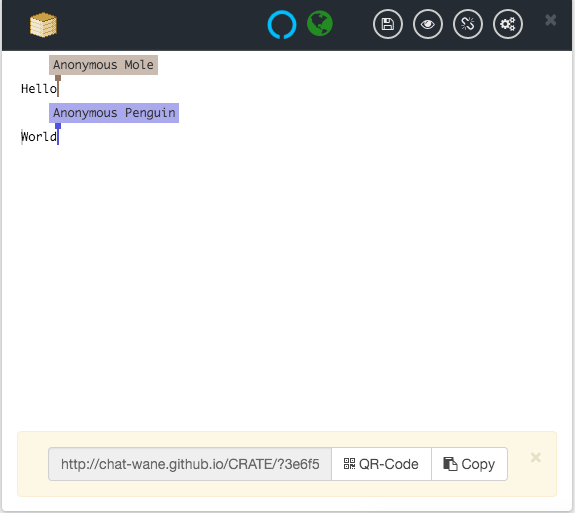
\includegraphics[scale=0.5]{img/editor/cratescreenshot.png}
    \caption{\label{editor:img:screenshot}Capture d'écran de \CRATE.}
  \end{center}
\end{figure}

La capture d'écran en figure~\ref{editor:img:screenshot} montre l'interface
visible par l'utilisateur. Dans cet exemple, au moins trois participants sont
impliqués dans la session d'édition. En effet, 3 curseurs sont affichés. Le
premier curseur appartient à \emph{Anonymous Mole} et semble être à l'origine du
texte \emph{Hello}. Le second curseur appartient à \emph{Anonymous Penguin} et
semble être à l'origine du texte \emph{World}. Le troisième curseur est celui de
l'utilisateur ayant prit la capture d'écran.

La barre d'état nous indique que
\begin{inparaenum}[(i)]
\item l'éditeur est en train de partager l'accès à la session d'édition via le
  cercle bleue en rotation. L'utilisateur peut alors donner l'URL en bas de page
  à d'autres collaborateurs afin qu'ils le rejoignent dans l'écriture du
  document, en un simple clique;
\item que l'utilisateur est bien connecté à d'autres collaborateurs via la
  planète verte.
\end{inparaenum}

La barre d'état possède aussi des boutons tels que
\begin{inparaenum}[(i)]
\item la disquette qui enregistre sur le disque la réplique locale du
  document. En ouvrant ce fichier, l'éditeur est capable de se réconnecter à la
  session d'édition sans avoir à rattrapper toutes les opérations qui lui manque
  depuis son départ;
\item l'oeil sert à visualiser le texte écrit dans le langage
  Markdown~\cite{markdown}. Ainsi, le document n'est plus une simple suite de
  caractères mais est interprété afin de présenter un document structuré plus
  agréable à lire;
\item la chaîne sert à partager l'accès au document ou à le stopper;
\item les engrenages servent à la configuration.
\end{inparaenum}


\subsection{Architecture}

\begin{figure}
  \begin{center}
    \begin{tikzpicture}[scale=1.2]

\newcommand\X{25pt}
\newcommand\Y{20pt}

\newcommand\LIGHTGRAY{gray!20}
\newcommand\MEDIUMGRAY{gray!40}

\small
%% communication
\draw[rounded corners=2mm, color=\MEDIUMGRAY, fill=white](0pt, 0pt)+(-4*\X,-\Y)rectangle+(4*\X,\Y);
\draw(4*\X, \Y)node[anchor=north east]{\textbf{communication}};

\draw[fill=white](-2*\X, -0.25*\Y)
node{broadcast}+(-0.75*\X,-0.5*\Y)rectangle+(0.75*\X,0.5*\Y);
\draw[fill=white, very thick]( 0*\X, 0.25*\Y)
node[align=center]{membership}+(-0.85*\X,-0.5*\Y)rectangle+(0.85*\X,0.5*\Y);
\draw[fill=white]( 2*\X, -0.25*\Y)
node{unicast}+(-0.75*\X,-0.5*\Y)rectangle+(0.75*\X,0.5*\Y);

\draw[<-](-0.85*\X, 0.25*\Y)--(-1.25*\X, -0.25*\Y);
\draw[<-](0.85*\X, 0.25*\Y)--(1.25*\X, -0.25*\Y);

%% causality
\draw[rounded corners=2mm, color=\MEDIUMGRAY, fill=\LIGHTGRAY](0pt, -2*\Y)+(-4*\X,-\Y)rectangle+(4*\X,\Y);
\draw(4*\X, -\Y)node[anchor=north east]{\textbf{causality}};

\draw[fill=\LIGHTGRAY](-2*\X, -2*\Y)
node[align=center]{semantic\\causality\\tracker}
+(-1.0*\X,-0.6*\Y)rectangle+(1.0*\X,0.6*\Y);
\scriptsize
\draw[->, thick](-1.5*\X, -0.75*\Y) -- node[anchor=west]{receive}
(-1.5*\X, -1.4*\Y);
\draw[<-, thick](-2.5*\X, -0.75*\Y) -- node[anchor=east]{send}
(-2.5*\X, -1.4*\Y);
\small
\draw[<->]( 2*\X, -0.75*\Y)--( 1*\X, -2.5*\Y);

%% sequence structure
\draw[rounded corners=2mm, color=\MEDIUMGRAY, fill=white](0pt, -4*\Y)+(-4*\X,-\Y)rectangle+(4*\X,\Y);
\draw(4*\X, -3*\Y)node[anchor=north east, align=right]
{\textbf{sequence}\\\textbf{structure}};

\draw[fill=white, shading=axis,top color=\LIGHTGRAY, bottom color=white, shading angle=0](1*\X, -3*\Y)
node{anti-entropy}+(-0.95*\X,-0.5*\Y) rectangle +(0.95 *\X, 0.5*\Y);
\draw[fill=white, very thick](-2*\X, -4*\Y)
node{replica}+(-0.75*\X,-0.5*\Y) rectangle +(0.75 *\X, 0.5*\Y);

\draw[->] (0.05*\X, -2.75*\Y)--(-1*\X,-2*\Y);
\draw[->] (0.05*\X, -3.25*\Y)--(-1.25*\X,-4*\Y);
\scriptsize
\draw[<-, thick] (-1.5*\X, -3.5*\Y)--node[anchor=west]{deliver}(-1.5*\X, -2.6*\Y);
\draw[->, thick] (-2.5*\X, -3.5*\Y)--node[anchor=east]{decorate}(-2.5*\X, -2.6*\Y);
\small
%% gui
\draw[rounded corners=2mm, color=\MEDIUMGRAY, fill=\LIGHTGRAY](0pt, -6*\Y)+(-4*\X,-\Y)rectangle+(4*\X,\Y);
\draw(4*\X, -5*\Y)node[anchor=north east, align=right]
{\textbf{graphical}\\\textbf{user}\\\textbf{interface}};
\draw[fill=\LIGHTGRAY](0pt,-6*\Y)
node{web editor}+(-0.85*\X,-0.5*\Y) rectangle +(0.85 *\X, 0.5*\Y);

%%\draw[<->] (-2*\X, -4.5*\Y) -- (0*\X, -5.5*\Y);
\scriptsize
\draw[->, thick] (-1.80*\X, -4.5*\Y)--node[anchor=west]{notify}(-0.85*\X, -5.75*\Y);
\draw[<-, thick] (-2.20*\X, -4.5*\Y)--node[anchor=east]{update}(-0.85*\X, -6.25*\Y);
\small
\end{tikzpicture}
    \caption{\label{editor:fig:architecture}Architecture en 4 couches de \CRATE.}
  \end{center}
\end{figure}

La figure~\ref{editor:fig:architecture} montre l'architecture en 4 couches de
\CRATE. Chacune de ces couches peut devenir un obstacle au passage à l'échelle
de l'éditeur :
\begin{inparaenum}[(i)]
\item la couche de communication comprend le méchanisme d'appartenance au réseau
  et la propagation des messages dans ce réseau;
\item la couche de causalité comprend la structure permettant de lier les
  opérations entre elles afin qu'elles soient intégrées dans un ordre reflétant
  une forme de causalité, e.g., elle assure que les opérations de suppression
  suivent toujours les opérations d'insertion de l'élément correspondant;
\item la couche de structure pour séquences dont les opérations d'insertions et
  de suppression doivent garantir des répliques convergeantes du document;
\item la couche d'interaction homme-machine fournissant les outils avec lesquels
  l'utilisateur peut intéragir.
\end{inparaenum}

La partie gauche de la figure montre le processus le plus courant : Lorsqu'un
participant effectue une opération sur le document, l'opération est appliquée à
la séquence répartie. L'opération est ensuite décorée avec des métadonnées
correspondant à la causalité. Enfin, l'éditeur propage l'opération en utilisant
le voisinage de l'éditeur fournit par le protocol d'appartenance au réseau.  À
l'inverse, lorsque l'éditeur reçoit une opération, il vérifie si cette dernière
est prête à être intégrée. Lorsque la condition est vérifiée, l'éditeur intégre
l'opération à la réplique de la séquence. Enfin l'interface utilisateur est
notifiée du changement.

La partie droite de la figure correspond à la stratégie de rattrapage où un
participant a peut-être manqué quelques opérations à cause de pertes de messages
dans le réseau, ou simplement car il était hors-ligne pendant un moment. Ainsi,
dès que l'éditeur est en ligne, il vérifie régulièrement auprès de ses voisins
s'il lui manque des opérations.

\subsection{Processus}

\begin{figure}
  \begin{center}
    
\begin{tikzpicture}[scale=1.1]

  \newcommand\X{30pt}
  \newcommand\Y{-30pt}

  \draw[->] (\X, 0)--(\X, 5+3*\Y); %% p1 p6
  \draw[->] (-5+2*\X, 0)--(5+\X, 0); %% p2 p1
  \draw[->] (2*\X, 0) -- (-5+3*\X, \Y); %% p2 p3
  \draw[->] (2*\X, 0) -- (-5+3*\X, 2*\Y); %% p2 p4
  \draw[->] (3*\X, 5+\Y) -- ( 5+2*\X, 0); %% p3 p2
  \draw[->] (3*\X, \Y) -- (5pt, 2*\Y); %% p3 p7
  \draw[->] (3*\X, \Y) -- (2*\X, 5+3*\Y); %% p3 p5
  \draw[->] (3*\X, 2*\Y) -- (5pt, 2*\Y); %% p4 p7
  \draw[->] (3*\X, 2*\Y) -- (5pt, \Y); %% p4 p8
  \draw[->] (2*\X, 3*\Y) -- (\X, -5pt); %% p5 p1
  \draw[->] (5+2*\X, 3*\Y) -- (3*\X, -5+ 2*\Y); %% p5 p4
  \draw[->] (-5+\X, 3*\Y) -- (0pt, -5+2*\Y); %% p6 p7
  \draw[->] (0pt, 2*\Y) -- (-5+3*\X, \Y); %% p7 p3
  \draw[->] (0pt, 2*\Y) -- (\X, -5pt); %% p7 p1
  \draw[->] (0pt, \Y) -- (2*\X, -5pt); %% p8 p2
  \draw[->] (0pt, \Y) -- (\X, 5+3*\Y); %% p8 p6
  \draw[->] (0pt, \Y) -- (-5+3*\X, \Y); %% p8 p3
  
  \draw[fill=white] (-2*\X, 1.5*\Y) node{$e_9$} +(-5pt,-5pt) rectangle +(5pt,5pt);
  \draw[<->, densely dashed] (-2*\X, 5+1.5*\Y) -- node[anchor=east]{join} (-2*\X, -5pt);

  \draw[fill=white] (-2*\X, 0) node{$mediator_1$} +(-20pt, -5pt)rectangle+(20pt, 5pt);
  \draw[<->, densely dashed] (20-2*\X, 0) -- node[anchor=south]{share} (-5+\X, 0);
  \draw[<->, densely dashed] (20-2*\X, -5pt) -- (-5pt, \Y);
  
  \draw[fill=white] (-2*\X, 3*\Y) node{$mediator_2$} +(-20pt, -5pt)rectangle+(20pt, 5pt);
  \draw[<->, densely dashed] (20-2*\X, 3*\Y) -- (-5+\X, 3*\Y);
  \draw[<->, densely dashed] (20-2*\X, 5+3*\Y) -- (-5pt, 2*\Y);

  \draw[fill=white] (\X, 0)node{$e_1$}+(-5pt, -5pt)rectangle+(5pt, 5pt);
  \draw[fill=white] (2*\X, 0)node{$e_2$}+(-5pt, -5pt)rectangle+(5pt, 5pt);
  \draw[fill=white] (3*\X, \Y)node{$e_3$}+(-5pt, -5pt)rectangle+(5pt, 5pt);
  \draw[fill=white] (3*\X, 2*\Y)node{$e_4$}+(-5pt, -5pt)rectangle+(5pt, 5pt);
  \draw[fill=white] (2*\X, 3*\Y)node{$e_5$}+(-5pt, -5pt)rectangle+(5pt, 5pt);
  \draw[fill=white] (1*\X, 3*\Y)node{$e_6$}+(-5pt, -5pt)rectangle+(5pt, 5pt);
  \draw[fill=white] (0 , 2*\Y)node{$e_7$}+(-5pt, -5pt)rectangle+(5pt, 5pt);
%  \draw[fill=white] (0 , \Y)+(-55pt, -10pt)rectangle+(5pt, 10pt);
  \draw[fill=white](0,\Y) node{$e_8$}+(-5pt, -5pt)rectangle+(5pt, 5pt);

\end{tikzpicture}
    \caption{\label{editor:fig:processus}Fonctionnement d'une session d'édition.}
  \end{center}
\end{figure}

\subsection{Anti-entropie}

%%% Local Variables:
%%% mode: latex
%%% TeX-master: "../../paper"
%%% End:



\section{Expérimentation}
\label{editor:sec:experimentation}


\begin{figure}
  \begin{center}
    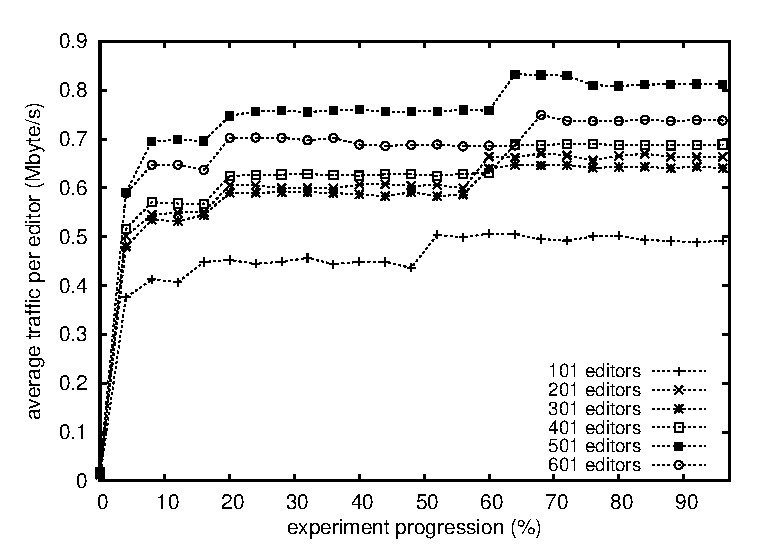
\includegraphics[width=0.8\textwidth]{img/editor/communication.eps}
    \caption[Trafic généré par \CRATE lors de sessions d'édition]
    {\label{editor:img:communication} Trafic moyen par seconde généré par chaque
      éditeur pendant la session d'édition. L'axe des abscisses montre la
      progression de l'expérimentation. L'axe des ordonnées montre le trafic
      moyen sortant par éditeur en mégaoctets par seconde.}
  \end{center}
\end{figure}

\paragraph{Objectif :} Montrer que l'éditeur collaboratif décentralisé \CRATE
passe à l'échelle en termes de nombre d'utilisateurs et de taille de
documents.

\paragraph{Description :} Cette expérimentation construit des réseaux de 101 à
601 participants. Pour cela, des machines sont réservées sur le banc d'essai
Grid'5000. Sur chacune d'elle sont lancées un à plusieurs navigateurs web
observant le processus d'intégration au réseau. Par exemple, 100 machines avec 6
navigateurs chacune permettent de créer le réseau à 601 participants -- le
participant supplémentaire étant le créateur du document hébergeant aussi le
serveur de signalisation.  Chaque session d'édition est en charge d'écrire un
document artificiel de plusieurs millions de caractères en insérant ceux-ci à la
fin du document. Les mesures concernent le trafic sortant moyen de chacun des
membres. Globalement, 100 opérations sont effectuées par seconde, uniformément
réparties entre les participants. La session dure 7 heures.

\paragraph{Résultat :} La figure~\ref{editor:img:communication} montre le
résultat de cette expérimentation.
\begin{inparaenum}[(i)]
\item Le trafic généré croît de façon polylogarithmique comparativement à la
  taille du document : Plus l'expérience progresse, plus le nombre d'insertions
  effectuées sur le document est important, plus la croissance des identifiants
  diminue.
\item À cela s'ajoute un facteur multiplicatif logarithmique comparé au nombre
  de participants : Plus la session d'édition comporte de membres, plus le trafic
  généré est important. Toutefois, l'écart entre les mesures diminues tandis que
  le nombre de participants est incrémenté linéairement. On note toutefois des
  exceptions à ces observations. Par exemple, les mesures sur 501 éditeurs
  dominent les mesures sur 601 éditeurs.
\end{inparaenum}

\paragraph{Explication :} \CRATE utilise \LSEQ
(cf. chapitre~\ref{repl:chap:lseq}). Le comportement d'édition des participants
est monotone. \LSEQ possède une complexité polylogarithmique sur ses
identifiants, comparé au nombre d'insertions effectuées dans la séquence. Ainsi,
plus les expérimentations progressent, plus le nombre d'insertions dans la
séquence augmente. Les messages envoyées ne comportant que les identifiants de
\LSEQ, la croissance du trafic hérite de cette croissance
polylogarithmique. \CRATE utilise \SPRAY
(cf. §\ref{net:chap:spray}). Lorsqu'un nouveau membre rejoins une
session d'édition, il apporte avec lui un nombre logarithmique de connexions par
rapport à la taille du réseau. Chacune ces connexions est activement utilisée
par le mécanisme de diffusion de messages afin que chacun des identifiants
parvienne à tous les éditeurs. Pour chaque opération locale effectuée, chaque
membre retransmet le message aux membres sa vue partielle exactement une
fois. D'où la progression logarithmique du trafic généré entre les sessions
d'édition. L'exception perçue entre certaines configurations de
l'expérimentation est due au coté aléatoire du protocole. Sur un grand nombre
d'exécution, cet aléatoire serait gommé.





\section{Conclusion}
\label{editor:sec:conclusion}

Ce chapitre a présenté \CRATE, un éditeur collaboratif décentralisé fonctionnant
directement dans les navigateurs Web. Un utilisateur peut créer, modifier en
temps réel et partager son document. À l'instar des éditeurs centralisés, tel
que Google Docs, le partage s'effectue très facilement grâce à un simple
lien. Lorsqu'un utilisateur clique sur celui-ci, il rejoint la session d'édition
et peut à son tour voir, modifier en temps réel et partager le document.

Ce que \CRATE ne gère pas : la persistance des sessions d'édition. De nos jours,
avec l'hégémonie des services hébergés sur le Nuage, il devient plus difficile
de supprimer des données que de les sauvegarder. À l'opposé, un document dans
\CRATE n'appartient qu'à ses rédacteurs. La session d'édition et donc le
document cessent d'exister lorsque tous les collaborateurs ferment leur
éditeur. Si ceux-ci souhaitent sauvegarder le document, ils peuvent le faire
localement. Si ceux-ci souhaitent préserver la session d'édition temps réel, ils
doivent s'assurer qu'au moins un éditeur reste actif et accessible.

\CRATE démontre que l'édition collaborative temps réel est possible dans les
navigateurs Web, sans l'intervention de tiers et sans limites quant aux
dimensions du système.

Le chapitre~\ref{conclu:chap:conclusion} revient sur les précédentes
contributions et présente les perspectives scientifiques ouvertes par celles-ci.

%%% Local Variables:
%%% mode: latex
%%% TeX-master: "../../paper"
%%% End:



\chapter{Conclusion}

\minitoc


\section{Conclusion}

%%% Local Variables:
%%% mode: latex
%%% TeX-master: "../../paper"
%%% End:


\section{Perspectives}
\label{conclu:sec:perspectives}

%Les travaux réalisés lors de cette thèse et présenté dans ce manuscrit offrent
%de nombreuses perspectives de différente granularité. 
Tout d'abord, chacun des composants de notre éditeur collaboratif peut être
amélioré ou étendu. Ensuite, l'éditeur lui-même offre des opportunités
inédites. Par exemple, son intégration, non en opposition, mais en complément
des approches actuellement centralisés. Enfin, l'architecture ouvre aussi la
voie à un plus large champs d'applications décentralisées directement
accessibles via les navigateurs Web.

Cette section fournit une liste de perspectives scientifiques concernant ces
travaux de thèse.

\subsection{Fusion de réseaux}

\label{conclu:subsec:merging}

La fusion de réseaux consiste à obtenir un réseau unique comme l'union des
membres de plusieurs réseaux. Le réseau obtenu doit hériter des propriétés de
ses parents.  Lors de ce processus, nous supposons qu'au moins un des nœuds
appartenant à l'un des réseau contacte l'autre réseau afin d'initier la
fusion. Grâce à la connexion qui en résulte, les réseaux sont à même de
communiquer, et donc de fusionner.

Les approches à taille fixe sont triviales à étendre : les mélanges périodiques
suffisent à garantir un réseau connexe. Si toutefois les vues partielles sont
configurées avec des tailles différentes, il suffit alors de prendre la taille
maximum des deux. Par exemple, un nœud avec une vue partielle de 5 voisins verra
sa vue augmenter à $7$ voisins après un échange avec le nœud dont la vue
partielle est peuplée de $7$ références.

\SPRAY est une approche dont les vues partielles évoluent automatiquement en
réaction aux entrées et sorties du réseau. En particulier, les vues partielles
suivent une progression logarithmiques comparée à la taille du réseau. La fusion
de réseaux \SPRAY doit résulter en un réseau \SPRAY garantissant de même.

La première solution qui vient à l'esprit est la suivante : chacun des nœuds du
premier réseau utilise le contact afin de rejoindre le second réseau, comme un
sablier dont les grains passent un tube étroit pour rejoindre l'autre bulbe sous
l'effet de la gravité. Malheureusement, cette solution est extrêmement lente --
puisque la majorité des nœuds ignorent encore qui est le contact -- et
susceptible d'échouer -- puisque le contact est un point unique de défaillance.

Un seconde solution consiste simplement, à l'instar des approches à taille fixe,
à laisser le mécanisme de mélange faire son office. Petit à petit, d'autres
ponts entre les réseaux vont se former jusqu'à ce que les deux réseaux soient
indifférenciés. Malheureusement, les arcs ne suivent pas l'augmentation relative
au réseau.

\begin{problem}
  Soit $\mathcal{N}_1,\, \mathcal{N}_2,\, \ldots ,\, \mathcal{N}_k$ des réseaux
  de taille arbitraire. On a :
\begin{equation}
  \sum\limits_{i \in \mathbb{N}_{<k}} |\mathcal{N}_i|\ln (|\mathcal{N}_i|) < (\sum\limits_{i \in \mathbb{N}_{<k}} |\mathcal{N}_i|)\ln{(\sum\limits_{i \in \mathbb{N}_{<k}} |\mathcal{N}_i|)}
\end{equation}
Comment adapter les nombres d'arcs effectif (à gauche) pour qu'il atteigne le
nombre d'arcs requis (à droite)?
\end{problem}


% Pour répondre à ce problème, chacun des nœuds appartenant aux réseaux impliqués
% dans la fusion doit être capable de
% \begin{inparaenum}[(i)]
% \item détecter lorsqu'un nouveau réseau fusionne avec celui dans lequel il se
%   trouve (cf. §\ref{net:subsec:detection}),
% \item détecter lorsqu'il a glané suffisamment d'informations pour procéder à la
%   fusion (cf. §\ref{net:subsec:activation}),
% \item ajuster sa vue partielle en conséquence (cf. §\ref{net:subsec:merging}).
% \end{inparaenum}

\subsection{Table de hachage répartie}

Une table de hachage répartie (\emph{DHT}\footnote{\emph{Distributed Hash
    Table}}) est un système permettant de retrouver une ressource rapidement
dans un réseau superposé de nœuds. La ressource recherchée possède une clé
permettant l'exploration efficace du réseau.

Parmi les représentants des DHT on trouve Chord~\cite{stoica2001chord},
CAN~\cite{ratnasamy2001scalable}, Pastry~\cite{rowstron2001pastry},
Tapestry~\cite{zhao2006tapestry}, Kademlia~\cite{maymounkov2002kademlia}, ou
Kelips~\cite{gupta2003kelips}.  Ces approches font souvent état d'une vue
partielle logarithmique.  Toutefois, tout comme pour les protocoles
d'échantillonnage aléatoire de pairs dont la vue partielle est fixe, tel que
\CYCLON, la taille de leur vue est configurée par avance. Lorsque le système
fait face à de fréquentes entrées et sorties de nœuds, les vues peuvent être
ajustées grâce à des mécanismes d'estimation de la taille du
réseau~\cite{camarillo2014self, ghinita2006adaptive}. Cependant, ces mécanismes
présentent un coût additionnel~\cite{ghinita2006adaptive}.

\begin{figure}
  \begin{center}
    
\begin{tikzpicture}[scale=1.2]

  \newcommand\X{75pt};
  \newcommand\Y{75pt};

  \newcommand\1{0.865};
  \newcommand\2{0.705};
  \newcommand\3{0.5};

  \scriptsize
  \draw[fill=white, very thick, draw=darkblue]
  (1*\X, 0*\Y) node{\DARKBLUE{$n_1$}} +(-5pt,-5pt) rectangle +(5pt,5pt);
  \draw[fill=white]
  (\1*\X, \3*\Y) node{$n_2$} +(-5pt,-5pt) rectangle +(5pt,5pt);
  \draw[fill=white]
  (\2*\X, \2*\Y) node{$n_3$} +(-5pt,-5pt) rectangle +(5pt,5pt);
  \draw[fill=white]
  (\3*\X, \1*\Y) node{$n_4$} +(-5pt,-5pt) rectangle +(5pt,5pt);
  \draw[fill=white]
  (0*\X, 1*\Y) node{$n_5$} +(-5pt,-5pt) rectangle +(5pt,5pt);
  
  \draw[->, very thick, color = darkblue](1*\X, 5+0*\Y) --
  node[anchor=west]{\DARKBLUE{\textbf{plus proche}}} (\1*\X, -5+\3*\Y);
  \draw[->](-5+\1*\X, 5+\3*\Y) -- (5+\2*\X, -5+\2*\Y);
  \draw[->](-5+\2*\X, 5+\2*\Y) -- (5+\3*\X, -5+\1*\Y);
  \draw[->](-5+\3*\X, \1*\Y) -- (5+0*\X, 1*\Y);


  \draw[fill=white]
  (-\3*\X, \1*\Y) node{$n_6$} +(-5pt,-5pt) rectangle +(5pt,5pt);
  \draw[fill=white]
  (-\2*\X, \2*\Y) node{$n_7$} +(-5pt,-5pt) rectangle +(5pt,5pt);
  \draw[fill=white]
  (-\1*\X, \3*\Y) node{$n_8$} +(-5pt,-5pt) rectangle +(5pt,5pt);
  \draw[fill=white]
  (-1*\X, 0*\Y) node{$n_9$} +(-5pt,-5pt) rectangle +(5pt,5pt);

  \draw[->](-5+0*\X, 1*\Y) -- (5+-\3*\X, \1*\Y);
  \draw[->](-5-\3*\X, -5+\1*\Y) -- (5-\2*\X, 5+\2*\Y);
  \draw[->](-5-\2*\X, -5+\2*\Y) -- (5-\1*\X, 5+\3*\Y);
  \draw[->](-\1*\X, -5+\3*\Y) -- (-1*\X, 5+0*\Y);

  \draw[fill=white]
  (-\1*\X, -\3*\Y) node{$n_{10}$} +(-5pt,-5pt) rectangle +(5pt,5pt);
  \draw[fill=white]
  (-\2*\X, -\2*\Y) node{$n_{11}$} +(-5pt,-5pt) rectangle +(5pt,5pt);
  \draw[fill=white]
  (-\3*\X, -\1*\Y) node{$n_{12}$} +(-5pt,-5pt) rectangle +(5pt,5pt);
  \draw[fill=white]
  (0*\X, -1*\Y) node{$n_{13}$} +(-5pt,-5pt) rectangle +(5pt,5pt);

  \draw[->](-1*\X, -5+0*\Y) -- (-\1*\X, 5-\3*\Y);
  \draw[->](5-\1*\X, -5-\3*\Y) -- (-5-\2*\X, 5-\2*\Y);
  \draw[->](5-\2*\X, -5-\2*\Y) -- (-5-\3*\X, 5-\1*\Y);
  \draw[->](5-\3*\X, -\1*\Y) -- (-5+0*\X, -1*\Y);

  \draw[fill=white]
  (\3*\X, -\1*\Y) node{$n_{14}$} +(-5pt,-5pt) rectangle +(5pt,5pt);
  \draw[fill=white]
  (\2*\X, -\2*\Y) node{$n_{15}$} +(-5pt,-5pt) rectangle +(5pt,5pt);
  \draw[fill=white]
  (\1*\X, -\3*\Y) node{$n_{16}$} +(-5pt,-5pt) rectangle +(5pt,5pt);

  \draw[->](5+0*\X, -1*\Y) -- (-5+\3*\X, -5-\1*\Y);
  \draw[->](5+\3*\X, -\1*\Y) -- (-5+\2*\X, -5-\2*\Y);
  \draw[->](5+\2*\X, 5-\2*\Y) -- (-5+\1*\X, -5-\3*\Y);
  \draw[->](\1*\X, 5-\3*\Y) -- (1*\X, -5+0*\Y);


  \draw[<->](0*\X, -5+1*\Y) -- (0*\X, 5+-1*\Y);
  \draw[<->](-5+\1*\X, -5+\3*\Y) -- (5-\1*\X, 5-\3*\Y);
  \draw[<->](-5+\2*\X, -5+\2*\Y) -- (5-\2*\X, 5-\2*\Y);
  \draw[<->](-5+\3*\X, -5+\1*\Y) -- (5-\3*\X, 5-\1*\Y);
  \draw[<->](-5+\1*\X, 5-\3*\Y) -- (5-\1*\X, -5+\3*\Y);
  \draw[<->](-5+\2*\X, 5-\2*\Y) -- (5-\2*\X, -5+\2*\Y);
  \draw[<->](-5+\3*\X, 5-\1*\Y) -- (5-\3*\X, -5+\1*\Y);


  \draw[->] (-5+\1*\X, \3*\Y) -- (5-\2*\X , \2*\Y); %% 2-> 7
  \draw[->] (-5+\2*\X, \2*\Y) -- (5-\1*\X, \3*\Y); %% 3 -> 8
%  \draw[->] (-5+\3*\X, -5+\1*\Y) -- (5-1*\X, 5+0*\Y); %% 4 -> 9
%  \draw[->] (-5+0*\X, -5+1*\Y) -- (5-\1*\X, 5-\3*\Y); %% 5 -> 10
  \draw[->] (-\3*\X, -5+\1*\Y) -- (-\2*\X, 5-\2*\Y); %% 6 -> 11
  \draw[->] (-\2*\X, -5+\2*\Y) -- (-\3*\X, 5-\1*\Y); %% 7 -> 12
  \draw[->] (5+-\1*\X, -5+\3*\Y) -- (-5+0*\X, 5-1*\Y); %% 8 -> 13
  \draw[->] (5+-1*\X, -5+0*\Y) -- (-5+\3*\X, 5-\1*\Y); %% 9 -> 14
  \draw[->] (5-\1*\X, -\3*\Y) -- (-5+\2*\X, -\2*\Y); %% 10 -> 15
%  \draw[->] (5-\2*\X, -\2*\Y) -- (-5+\1*\X, -\3*\Y); %% 11 -> 16
  \draw[->] (5-\3*\X, 5-\1*\Y) -- (-5+1*\X, -5+0*\Y); %% 12 -> 1
%  \draw[->] (5-0*\X, 5-1*\Y) -- (-5+\1*\X, -5+\3*\Y); %% 13 -> 2
  \draw[->] (\3*\X, 5-\1*\Y) -- (\2*\X, -5+\2*\Y); %% 14 -> 3
  \draw[->] (\2*\X, 5-\2*\Y) -- (\3*\X, -5+\1*\Y); %% 15 -> 4
  \draw[->] (-5+\1*\X, 5-\3*\Y) -- (5+0*\X, -5+1*\Y); %% 16 -> 5


  \draw[<->, very thick, color = darkblue](5-\X, 0*\Y) --
  node[anchor=south west]{\DARKBLUE{\textbf{\ \ \ \ plus lointain}}}(-5+\X, 0*\Y);
  \draw[->, very thick, color = darkblue] (-5+\X, 5+0*\Y) --
  node[anchor=south]{\DARKBLUE{$\mathbf{1\over{3}}$}}(5-\3*\X, -5+\1*\Y); %% 1 -> 6
\end{tikzpicture}


%%% Local Variables:
%%% mode: latex
%%% TeX-master: "../../paper"
%%% End:

    \caption[Table de hachage répartie]
    {\label{conclu:fig:dhtexample}Table de hachage répartie suivant le principe
      de Chord.}
  \end{center}
\end{figure}

Construire une DHT au dessus d'un protocole d'échantillonnage aléatoire de pairs
apporte le double avantage d'une convergence rapide vers une topologie optimale,
et d'une résilience aux fréquentes entrées et sorties de
nœuds~\cite{krasikova2016distributed, montresor2005chord,
  voulgaris2013vicinity}.  Comme le montre la
figure~\ref{conclu:fig:dhtexample}, l'idée est de placer les systèmes classiques
de DHT -- ici Chord -- afin qu'ils s'accordent avec la vue partielle fournie par
\SPRAY. Par exemple, si un nœud \SPRAY possède 3 voisins, le réseau superposé en
charge de la DHT possède lui aussi 3 voisins. Toutefois, ces derniers sont
choisis selon la distance à laquelle ils se trouvent. Un premier voisin serait
celui qui est le plus proche, le second voisin celui qui se trouve à la moitié
de la distance maximum, et le troisième se trouverait à un tiers de la distance
maximum. Un tel système permet de diriger les messages ciblant un nœud
particulier très efficacement : de l'ordre de $\log |\mathcal{N}|$ sauts en
moyenne, où $\mathcal{N}$ est l'ensemble des membres appartenant au réseau.

% \subsection{Sécurité}

% Les protocoles d'appartenance à un réseau font face à des problèmes de sécurités
% inhérents aux protocoles ciblant de larges dimensions. 

\subsection{Compromis causalité et concurrence}

\CRATE comprend une couche dédiée à la détection de relations causales. La
structure utilisée est celle d'un vecteur d'horloges incluant des
exceptions~\cite{malkhi2007concise}. Celle-ci, identiquement aux vecteurs
d'horloges, stockent localement au moins un entier par collaborateur ayant
jamais participé dans l'édition. Pour les dispositifs informatiques aux
configurations plus modestes comme les téléphones portables, la progression
linéaire de ces vecteurs constitue un problème.

Une perspective possible serait de remplacer ce vecteur d'horloges de taille
$W$, où $W$ est le nombre de membres ayant jamais participé à la session
d'édition, par un vecteur d'horloges de taille $K$, où $K$ est un entier
nettement inférieur à $W$. L'intuition derrière cette structure provient du fait
que lorsqu'il n'y a pas de concurrence, une seule horloge de
Lamport~\cite{lamport1978time} suffit pour caractériser les relations
causales. Si la concurrence augmente, alors des doublons peuvent
apparaître. L'intégration, en présence de doublons, peut conduire à des
incohérences.

L'idée serait alors d'allier
\begin{inparaenum}[(i)]
\item une structure utilisant un vecteur dont la taille s'ajuste à la
  concurrence du système afin de borner la fréquence des erreurs;
\item un mécanisme de recouvrement sur erreur afin d'intégrer l'opération
  arrivée en retard;
\item un mécanisme d'anti-entropie afin que le système soit fiable : toutes les
  opérations parviennent à tous les participants.
\end{inparaenum}

% \subsection{Wiki réparti temps réel}

% Les wikis sont des espaces de collaborations permettant à plusieurs participants
% d'éditer des pages à tour de rôle, i.e., l'édition n'est pas effectuée en temps
% réel. Le succès de l'encyclopédie \emph{Wikipédia}~\cite{wikipedia} n'est plus à
% démontrer~\cite{giles2005internet}. Cependant, le modèle même d'édition provoque
% l'apparition de conflits. Ces conflits ne concernent pas seulement des points de
% vue divergents, mais aussi des éditions placées aux même endroit dans le
% document au même moment. Les conflits doivent être résolus manuellement ce qui
% constitue une tâche complexe à tel point que les discussions quant à
% l'organisation de la rédaction ont énormément augmenté au cours du
% temps~\cite{kittur2007he}.

% Autoriser l'édition temps réel des pages de \emph{Wikipédia} permettrait à
% différent utilisateurs de voir les modifications effectués par d'autres
% collaborateurs afin d'agir en conséquence. Dans ce cas, les seuls conflits
% restants seraient ceux d'ordre sémantique.  De plus, décentraliser ces sessions
% d'édition temps réel permettrait de soulager le fournisseur du service des coûts
% liés à l'édition. Les membres d'une session d'édition participeraient seuls au
% bon fonctionnement de la session. Une fois le travail accompli, le document est
% sauvegardé sur le serveur et versionné normalement. Seul la sauvegarde finale
% reste de sa responsabilité.

% Enfin, \CRATE permet de placer des liens à d'autres sessions d'édition dans le
% document. Ce simple mécanisme permet de naviguer d'un document à l'autre, d'une
% session d'édition à l'autre, et plus généralement d'un réseau à un autre. Il est
% alors possible de naviguer très simplement parmi ces réseaux, pour peu qu'ils
% soient encore vivants et accessibles.

% Certains projets, comme \emph{The Fold}
% bénéficient d'une foule de gens volontaires qui mettent leur machine à
% disposition afin d'améliorer la puissance calculatoire du système.

\subsection{O'Browser, Where Art Thou?}

De nos jours, les navigateurs Web sont plus que de simples visualisateurs de
contenu, ils sont presque devenus des systèmes d'exploitation. Ils comptent
parmi les programmes les plus distribués de par le monde. Ils apparaissent dans
un large éventail d'appareils aux diverses capacités tels que les mobiles, les
tablettes, ou les ordinateurs de bureaux.

Développer une application Web, c'est développer pour une large audience
hétérogène.  L'éditeur collaboratif temps réel \CRATE prouve qu'il est possible
de développer des applications décentralisées directement dans le navigateur
Web. Le projet WebTorrent~\cite{webtorrent} constitue un autre exemple
d'application décentralisée fonctionnant dans le navigateur Web. Ce projet
permet le transfert de fichiers statique. Quelles autres applications
décentralisées est-il possible de développer ?

Rassembler l'ensemble des composants répartis en un langage adapté au Web
permettrait de développer un catalogue d'applications décentralisées
garantissant certaines propriétés sur, par exemple, le critère de cohérence ou
la sécurité. \CRATE ne serait que l'une des applications temps réel que ce
langage permettrait d'écrire. Cela constituerait une avancée certaine en faveur
d'un Web décentralisé. De surcroît, lorsque des navigateurs Web sont
actuellement entièrement développés dans l'optique de supporter le
décentralisé~\cite{maelstrom} -- ce qui représente une dépense substantielle --
le même objectif pourrait être atteint en étendant simplement les capacités des
navigateurs Web existants.


%%% Local Variables:
%%% mode: latex
%%% TeX-master: "../../paper"
%%% End:


%%% Local Variables:
%%% mode: latex
%%% TeX-master: "../../paper"
%%% End:


\bibliographystyle{plain}
\bibliography{bibliographie}

%\backmatter
\end{document}

%%% Local Variables:
%%% mode: latex
%%% End: